\documentclass[10pt,twocolumntoc]{cekarticle}
\usepackage{amsmath}
\usepackage{amssymb}
\usepackage{array}
\latexhtml{
  \usepackage[american]{varioref}
}{
  \newcommand{\vref}[1]{\ref{#1}}
}

% Aliases for bibliography entries, to compensate for some issues.

\defcitealias{bipm:1998}{BIPM, 1998}
\defcitealias{bipm:2000}{BIPM, 2000}


% Miscellaneous macros.

\newcommand{\D}{\displaystyle}
\newcommand{\tm}{\textsuperscript{\tiny{\texttrademark}}}

\newcommand{\quantity}[1]{\emph{#1}}
\newcommand{\unit}[1]{\texttt{#1}}

\begin{document}

%=============================================================================
% Title page
%=============================================================================

\title{Systems Biology Markup Language (SBML) Level 2:\\
  Structures and Facilities for Model Definitions}

\author{Andrew Finney, Michael Hucka}

\authoremail{\{afinney,mhucka\}@cds.caltech.edu}

\address{Systems Biology Workbench Development Group\\
  ERATO Kitano Symbiotic Systems Project\\
  Control and Dynamical Systems, MC 107-81\\
  California Institute of Technology, Pasadena, CA 91125, USA\\[3pt]
  \url{http://www.cds.caltech.edu/erato}}

\acknowledge{Principal Investigators: John Doyle and Hiroaki Kitano}

\date{SBML Level 2, Version 1 (Final Draft)\\[5pt]
  \today{}}

\maketitlepage


%=============================================================================
\section{Introduction}
\label{sec:introduction}
%=============================================================================

We present the \textbf{S}ystems \textbf{B}iology \textbf{M}arkup
\textbf{L}anguage (SBML) Level~2, a model representation formalism for
systems biology.  SBML is oriented towards describing systems of
biochemical reactions of the sort common in research on a number of topics,
including cell signaling pathways, metabolic pathways, biochemical
reactions, gene regulation, and many others.  SBML is defined in a neutral
fashion with respect to programming languages and software encoding;
however, it is primarily oriented towards allowing models to be encoded
using XML, the eXtensible Markup Language~\citep{bosak:1999,bray:2000}.
This document contains many examples of SBML models written in XML, as well
as an XML Schema~\citep{biron:2000,fallside:2000,thompson:2000} that
defines SBML Level~2.  A downloadable copy of the XML Schema and other
related documents and software are also available from the SBML project web
site, \url{http://www.sbml.org/}.

Major releases of SBML are termed \emph{levels}.  SBML Level 2 evolved out
of SBML Level~1~\citep{hucka:2001,hucka:2003}.  All of the structures of
Level 1 can be mapped in a straightforward fashion to Level~2.  In
addition, a large subset of the structures in Level~2 can be mapped to
Level~1.  However, the levels remain distinct; a valid SBML Level~1
document is not a valid SBML Level~2 document, and likewise, a valid SBML
Level~2 document is not a valid SBML Level~1 document.
Appendix~\ref{apdx:level1-level2} lists the differences between
Level~1 and Level~2.

SBML Level 2 was created in collaboration
with the authors of the following systems:
\emph{BASIS}~\citep{kirkwood:2003},
\emph{BioSkektchPad}~\citep{belta:2003},
\emph{BioSpice}~\citep{arkin:2001},
\emph{CellDesigner}~\citep{funahashi:2003},
\emph{Cellerator}~\citep{shapiro:2001,shapiro:2003b},
\emph{COPASI}~\citep{mendes:2000},
\emph{DBSolve}~\citep{goryanin:2001,goryanin:1999},
\emph{E-Cell}~\citep{tomita:1999,tomita:2001},
\emph{ESS}~\citep{peterson:2003},
\emph{Gepasi}~\citep{mendes:1997,mendes:2001},
\emph{Jarnac}~\citep{sauro:2000,sauro:1991},
\emph{JDesigner}~\citep{sauro:2001b},
\emph{JigCell}~\citep{vass:2003},
\emph{MCell}~\citep{bartol:2002},
\emph{NetBuilder}~\citep{schilstra:2002},
\emph{ProMot/DIVA}~\citep{stelling:2001},
\emph{StochSim}~\citep{bray:2001,morton-firth:1998}, and
\emph{Virtual Cell}~\citep{schaff:2000,schaff:2001}.
SBML Level~2 was developed with
the help of these packages' authors, as well as help and collaboration from
the creators of CellML~\citep{hedley:2001b} and many other individuals
listed in the Acknowledgments (Section~\ref{sec:acknowledgements}).


%-----------------------------------------------------------------------------
\subsection{Scope and Limitations}
%-----------------------------------------------------------------------------

SBML Level 2 is meant to support basic biochemical network models and the
kinds of operations that are possible in existing analysis/simulation
tools.  Future software tools will undoubtedly require further evolution of
SBML, and we expect that higher SBML levels will add structures and
facilities on top of Level~2 after the simulation community has had time to
gain experience with the current language definition.  In
Section~\ref{sec:level-3}, we discuss extensions that will likely be
included in SBML Level~3.

The definition of the model description language presented here does not
specify \emph{how} programs should communicate or read/write SBML.  We
assume that for a simulation program to communicate a model encoded in
SBML, the program will have to translate its internal data structures to
and from SBML, use a suitable transmission medium and protocol, etc., but
these issues are outside of the scope of this document.

%-----------------------------------------------------------------------------
\subsection{Notational Conventions}
%-----------------------------------------------------------------------------

We define SBML using a graphical notation based upon UML, the Unified
Modeling Language~\citep{eriksson:1998,oestereich:1999}.  This UML-based
definition in turn is used to define an XML
Schema~\citep{biron:2000,fallside:2000,thompson:2000} for SBML.  There are
three main advantages to using UML as a basis for defining SBML data
structures.  First, compared to using other notations or a programming
language, the UML visual representations are generally easier to grasp by
readers who are not computer scientists.  Second, the visual notation is
implementation-neutral: the defined structures can be encoded in any
concrete implementation language---not just XML, but C or Java as well.
Third, UML is a de facto industry standard that is documented in many
sources.  Readers are therefore more likely to be familiar with it than
other notations.

Our notation and our approach for mapping it to XML Schemas is explained in
a separate document~\citep{hucka:2000b}.  A summary of the essential points
is presented in Appendix~\ref{apdx:notation}, and examples throughout this
document illustrate the approach.  All types in SBML follow XML schema
datatype definitions and conventions.

We follow certain naming and
typographical conventions throughout this document.  Specifically, the
names of data structure attributes or fields begin with a lowercase letter,
and the names of data structures and types begin with an uppercase letter.
Keywords (names of types, XML elements, etc.) are written in a
typewriter-style font; for example, \class{Compartment} is a type name and
\class{compartment} is a field name.  Likewise, literal XML examples are
also written in a typewriter-style font.


%=============================================================================
\section{Overview of SBML}
\label{sec:overview}
%=============================================================================

The following is an example of a simple, hypothetical network of
biochemical reactions that can be represented in SBML:
\begin{equation*}
  \begin{array}{@{}ccl@{}}
    S_1 & \underrightarrow{k_1 [S_1] / ([S_1] + k_2)} & S_2 \\ \\[-3pt]
    S_2 & \underrightarrow{k_3 [S_2]} & S_3 + S_4
  \end{array}
\end{equation*}
Broken down into its constituents, this model contains a number of
components: reactant species, product species, reactions,
rate laws, and parameters in the rate laws.  To analyze or
simulate this network, additional components must be made
explicit, including compartments for the species, and units on the
various quantities.  The top level of an SBML model definition
simply consists of lists of these components:
\begin{center}
  \slshape
  \begin{tabular}{c}
    \begin{minipage}{3in}
      \begin{tabbing}
        xxxx\=xxxx\=xxxx\=xxxx\=\kill
        beginning of model definition\\
        \>list of function definitions (optional)\\
        \>list of unit definitions (optional)\\
        \>list of compartments (optional)\\
        \>list of species (optional)\\
        \>list of parameters (optional)\\
        \>list of rules (optional)\\
        \>list of reactions (optional)\\
        \>list of events (optional)\\
        end of model definition
      \end{tabbing}
    \end{minipage}
  \end{tabular}
\end{center}
The meaning of each component is as follows:
\begin{description}

\item \emph{Function definition}: A named function that may be used
  throughout the rest of the model.
    
\item \emph{Unit definition}: A name for a unit used in the expression of
  quantities in a model.  Units may be supplied in a number of contexts in
  an SBML model, and it is convenient to have a facility for both setting
  default units and for allowing combinations of units to be given
  abbreviated names.

\item \emph{Compartment}: A container of finite size for substances.  In
  SBML Level~2, a compartment is primarily a topological structure with size
  but no geometric qualities.
  
\item \emph{Species}: A substance or entity that takes part in a reaction.
  Some example species are ions such as $\text{Ca}^{2+}$ and molecules such
  as glucose or ATP.  The primary qualities associated with a chemical
  species in SBML Level~2 are its initial amount and the compartment in
  which it is located.
  
\item \emph{Parameter}: A quantity that has a symbolic name.  SBML Level~2
  provides the ability to define parameters that are global to a model as
  well as parameters that are local to a single reaction.
 
\item \emph{Rule}: In SBML, a mathematical expression that is used in
  combination with the differential equations constructed based on the set
  of reactions; it can be used to establish constraints between variables in
  a model, define how a variable can be calculated from other variables,
  or used to define the rate of change of a variable.

\item \emph{Reaction}: A statement describing some transformation,
  transport or binding process that can change the amount of one or more
  species.  For example, a reaction may describe how certain entities
  (reactants) are transformed into certain other entities (products).
  Reactions have associated rate laws describing how quickly they take
  place.
  
\item \emph{Event}: A statement describing an instantaneous, discontinuous
  transformation of a set of variables of any type (species concentration,
  compartment size or parameter value) when some triggering condition is
  satisfied. 
\end{description}

A software package can read an SBML model description and translate it
into its own internal format for model analysis.  For example, a package
might provide the ability to simulate the model by constructing
differential equations representing the network and then perform
numerical time integration on the equations to explore the model's dynamic
behavior.

SBML allows models of arbitrary complexity to be represented.  Each type of
component in a model is described using a specific type of data structure
that organizes the relevant information.  The data structures determine how
the resulting model is encoded in XML.

In the sections that follow, the various constructs in SBML and their uses
are described in detail.  Section~\ref{sec:general} first introduces a few
basic structures that are used throughout SBML Level~2, then
Section~\ref{sec:elements} provides details on each of the main components.
Section~\ref{sec:xml-rep} provides a number of complete examples of models
encoded in XML using SBML Level~2.  Section~\ref{sec:discussion} contains a
list of anticipated enhancements that will be made in SBML Level 3 and a
discussion of other efforts related to SBML.  Appendix~\ref{apdx:notation}
summarizes the UML-based notation used in this document.
Appendix~\ref{apdx:level1-level2} describes the differences between SBML Level~1
Version~2 and SBML Level~2 as described in this document and
Appendix~\ref{apdx:schema} provides the complete XML Schema for SBML
Level~2.


%=============================================================================
\section{Preliminary Definitions}
\label{sec:general}
%=============================================================================

This section covers certain concepts and constructs that are used
repeatedly in the rest of SBML Level 2 and are useful to discuss before
diving into the details of the data structures provided in SBML Level 2.

%-----------------------------------------------------------------------------
\subsection{Type \class{SBase} and the SBML Type Inheritance Hierarchy}
\label{sec:sbase}
%-----------------------------------------------------------------------------

Every structure composing an SBML Level 2 model definition has a specific
data type that is derived directly or indirectly from a single abstract
type called \class{SBase}.  This base type is designed to allow a modeler
or a software package to attach arbitrary information to each major
structure or list in an SBML model.  The definition of \class{SBase} is presented
in Figure~\vref{fig:sbase}.

\begin{figure}[ht]
  \vspace*{10pt}                        % ADJUSTMENT FOR THIS PAGE
  \centering
  
\includegraphics[scale = 0.68]{sbase}
  \caption{The definition of \class{SBase}.  Text enclosed in braces next
    to attribute types (e.g., \attribtype{\{minOccurs="0"\}}) indicates
    constraints on the possible attribute values.  We use XML Schema
    language to express constraints since we are primarily interested in
    the XML encoding of SBML.  The constraint expression
    \attribtype{use="optional"} means that the indicated field is optional
    and may be omitted in a particular instance in a model.  The constraint
    expression \attribtype{minOccurs="0"} likewise means that the indicated
    field is optional; this alternate form of expression must be used in
    XML Schema for those fields that are containers (i.e., fields that are
    encoded as subelements in XML).}
  \label{fig:sbase}
\end{figure}

\class{SBase} contains three fields, all of which are optional:
\attrib{metaid}, \attrib{notes} and \attrib{annotation}.

\subsubsection{The \attrib{metaid} Field}

The \attrib{metaid} field is present for supporting metadata annotations
using RDF.  It has a data type of \class{ID} (the XML identifier type), and
serves as anchors for metadata references.  Metadata expressed using RDF
can be placed anywhere within an \class{sbml} element and its subelements,
\emph{except} within MathML elements.  The metadata elements can include
RDF \class{description} elements in which the RDF \attrib{describes}
attributes contain the values of the \attrib{metaid} fields of SBML
elements in the model.  The form of the RDF element content in SBML should
follow the form described in the CellML Metadata
Specification~\citep{cuellar:2002}.

\subsubsection{The \attrib{notes} Field}

The field \attrib{notes} in \class{SBase} is a container for XHTML content.
It is intended to serve as a place for storing optional information
intended to be seen by humans.  Typically the \attrib{notes} field will contain
user comments about the structure in which the \attrib{notes} field is enclosed.
Every data object derived directly or
indirectly from type \class{SBase} can have a separate value for
\attrib{notes}, allowing users considerable freedom when adding comments to their
models.

\subsubsection{The \attrib{annotation} Field}

\class{SBase} includes the field called \attrib{annotation} to
provide a container for software-generated annotations that are \emph{not}
intended to be seen by humans.  This field is a container for arbitrary
data (XML type \class{any}).  As with the user-visible \attrib{notes}
field, every data object can have its own value for \attrib{annotation}.
Guidelines for using this field are given in Section~\ref{sec:annotation-use}.

\subsubsection{The SBML Type Inheritance Hierarchy}

The overall SBML inheritance hierarchy is depicted in
Figure~\vref{fig:top-level}.  In addition to the relationships shown, all
substructures such as \attrib{trigger} on \class{Event} and the
\class{listOf}\rule{0.5in}{0.5pt} lists are also derived from
\class{SBase}.  (However, the \attrib{notes} and \attrib{annotation}
elements contained inside \class{SBase} are not derived from
\class{SBase}.)

\begin{figure}[ht]
  \vspace*{8pt}
  \centering
  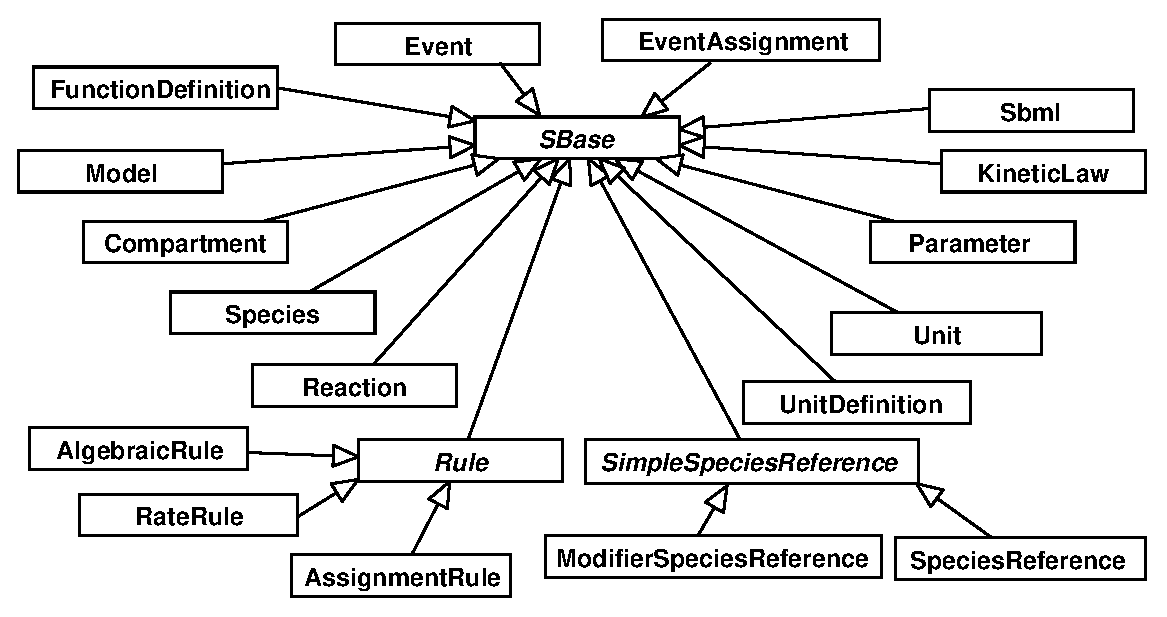
\includegraphics[scale = 0.7]{top-level}
  \caption{A UML diagram of the inheritance hierarchy of major data types
    in SBML.  Open arrows indicate inheritance, pointing from inheritors to
    their parents~\citep{eriksson:1998,oestereich:1999}.}
  \label{fig:top-level}
\end{figure}

%In the other SBML type definitions presented below, we follow the UML
%convention of hiding the attributes derived from a parent type such as
%\class{SBase}. It should be kept in mind that these attributes are always
%available.


%-----------------------------------------------------------------------------
\subsection{Guidelines for the Use of the \attrib{annotation} Field in
  \class{SBase}}
%-----------------------------------------------------------------------------
\label{sec:annotation-use}

The \attrib{annotation} field in the definition of \class{SBase} is
formally unconstrained in order that software developers may attach any
information they need to the structures in an SBML model.  However, it
is important that this facility not be misused.  In
particular, it is critical that information essential to a model definition
is \emph{not} stored in \attrib{annotation}.  Parameter values, functional
dependencies between model structures, etc., should not be recorded as
annotations.

Here are examples of the kinds of data that may be appropriately
stored in \attrib{annotation}: (a) information about the graphical
layout of model components; (b) application-specific processing
instructions that do not change the essence of a model; (c)
identification information for cross-referencing components in a
model with items in a database.

Different applications may use XML Namespaces~\citep{bray:1999} to specify
the intended vocabulary of a particular annotation.  Here is an example.
Suppose a particular application needs to annotate data structures in an
SBML model definition with screen layout information and a time stamp.  The
application's developers should choose a URI (\emph{Universal Resource
  Identifier}; \citealt{harold:2001,w3c:2000}) reference that uniquely
identifies the vocabulary the application will use for such annotations,
and a prefix string for the annotations.  For illustration purposes, let us
say the URI reference is ``\texttt{http://www.mysim.org/ns}'' and the
chosen prefix is \texttt{mysim}.  An example of an annotation might then be
as follows:

\begin{example}
...
<annotation xmlns:mysim="http://www.mysim.org/ns">
    <mysim:nodecolors mysim:bgcolor="green" mysim:fgcolor="white"/>
    <mysim:timestamp>2000-12-18 18:31 PST</mysim:timestamp>
</annotation>
...
\end{example}

The namespace prefix \texttt{mysim} is used to qualify the XML elements
\texttt{mysim:nodecolors} and \texttt{mysim:timestamp}; presumably these
symbols have meaning to the application.  This example places the XML
Namespace information on \attrib{annotation} itself rather than on a
higher-level enclosing construct or the enclosing document level, but other
placements would be valid as well~\citep{bray:1999}.

The use of XML Namespaces permits multiple applications to place
annotations on XML elements of a model without risking interference or
element name collisions.  Annotations stored by different simulation
packages can thus coexist in the same model definition.  Although XML
Namespace names 
must be URI references, an XML Namespace name is \emph{not required} to be
directly usable in the sense of identifying an actual, retrieval document
or resource on the Internet~\citep{bray:1999}.
``\texttt{http://www.mysim.org/}'' is a namespace name or URI in the example 
above.  The name is simply intended
to enable unique identification of constructs, and using URIs is a common
and simple way of creating a unique name string.  For the convenience of
developers of simulation and analysis tools, we reserve certain namespace
names for use with annotations in SBML.  These reserved names are listed in
Table~\vref{tab:reserved-urls}.

\begin{table}[b]
  \vspace*{10pt}
  \small
  \centering
  \begin{tabular}{ll}
    \toprule
    \texttt{http://www.sbml.org/2001/ns/basis}      & \texttt{http://www.sbml.org/2001/ns/jdesigner}\\
    \texttt{http://www.sbml.org/2001/ns/biocharon}  & \texttt{http://www.sbml.org/2001/ns/jigcell}\\
    \texttt{http://www.sbml.org/2001/ns/bioreactor} & \texttt{http://www.sbml.org/2001/ns/jsim}\\
    \texttt{http://www.sbml.org/2001/ns/biosketchpad}   & \texttt{http://www.sbml.org/2001/ns/libsbml}\\
    \texttt{http://www.sbml.org/2001/ns/biospice}   & \texttt{http://www.sbml.org/2001/ns/mathsbml}\\
    \texttt{http://www.sbml.org/2001/ns/celldesigner}   & \texttt{http://www.sbml.org/2001/ns/mcell}\\
    \texttt{http://www.sbml.org/2001/ns/cellerator} & \texttt{http://www.sbml.org/2001/ns/netbuilder}\\
    \texttt{http://www.sbml.org/2001/ns/copasi}     & \texttt{http://www.sbml.org/2001/ns/pathdb}\\
    \texttt{http://www.sbml.org/2001/ns/cytoscape}  & \texttt{http://www.sbml.org/2001/ns/promot}\\
    \texttt{http://www.sbml.org/2001/ns/dbsolve}    & \texttt{http://www.sbml.org/2001/ns/sbedit}\\
    \texttt{http://www.sbml.org/2001/ns/ecell}      & \texttt{http://www.sbml.org/2001/ns/sigpath}\\
    \texttt{http://www.sbml.org/2001/ns/gepasi}     & \texttt{http://www.sbml.org/2001/ns/stochsim}\\
    \texttt{http://www.sbml.org/2001/ns/isys}       & \texttt{http://www.sbml.org/2001/ns/vcell}\\
    \texttt{http://www.sbml.org/2001/ns/jarnac}     & \texttt{http://www.sbml.org/2001/ns/winscamp}\\
    \bottomrule
  \end{tabular}
  \caption{Reserved XML Namespace names in SBML Level 2.}
  \label{tab:reserved-urls}
\end{table}

Note that the namespaces being referred to here are XML Namespaces
specifically in the context of the \attrib{annotation} field on
\class{SBase}.  The namespace issue here is unrelated to the namespaces
discussed in Section~\ref{sec:namespaces} in the context of
\class{SId} and symbols in SBML.

%-----------------------------------------------------------------------------
\subsection{The \attrib{id} and \attrib{name} Fields on SBML Components}
\label{sec:idnameattribs}
%-----------------------------------------------------------------------------

As will become apparent below, most structures in SBML include two common
fields: \attrib{id} and \attrib{name}.  The \attrib{id} field is usually
required for most structures and is used to identify a component within the
model definition.  Other SBML structures can refer to the component using
this identifier.  Section~\ref{sec:id} defines the data type \class{SId}
used for the \attrib{id} field, and Section~\ref{sec:namespaces} describes
the scoping and namespace rules for these identifiers.
The equality of \class{SId} values is determined by an exact character sequence
match, i.e. in a
case sensitive manner, this applies to all uses of \class{SId} including
the identification of unit definitions.

In contrast to the \attrib{id} field, the \attrib{name} field is optional
and is not intended to be used for cross-referencing purposes within a
model.  Its purpose instead is to provide a human-readable label for the
component.  The data type of the \attrib{name} field is the type
\class{string} defined in XML Schema~\citep{biron:2000,thompson:2000}.
This type includes all Unicode characters~\citep{unicode:1996} except for
two delimiter characters, 0xFFFE and 0xFFFF~\citep{biron:2000}.  
The ampersand (\texttt{\&}) character must be escaped (using the entity \texttt{\&amp;}).
The apostrophe (\texttt{"}) or  single-quote character (\texttt{'}) characters must be
escaped (using the entities \texttt{\&apos;} or \texttt{\&quot;} respectively) when
those characters are used to delimit a string attribute value.
Other XML built-in character or entity references e.g \texttt{\&lt;} or \texttt{\&x1A;}
can be used. 
No
restrictions as to the content of \attrib{name} fields are imposed by SBML
beyond those defined by the \class{string} type of XML Schema.

The recommended practice for handling \attrib{name} is as follows.  If a
software tool has the capability for displaying the content of
\attrib{name} fields, it should display this content to the user as a
component's label instead of the component's \attrib{id} field.  If the
user interface does not have this capability (e.g., because it cannot
display or use special characters in symbol names), or if the \attrib{name}
field is missing on a given component, then the user interface should
display the value of the \attrib{id} field instead.  (Script language
interpreters are especially likely to display \attrib{id} fields instead of
\attrib{name} fields.)

As a consequence of the above, authors of systems that automatically
generate the values of \attrib{id} fields should be aware some systems may
display the \attrib{id}'s to the user.  Authors therefore may wish to take
some care to have their software create \attrib{id} values that are easy
for humans to type and read.

An additional point worth mentioning is although there are restrictions on
the uniqueness of \attrib{id} values (see Section~\ref{sec:namespaces}
below), there are no restrictions on the uniqueness of \attrib{name} values
in a model.  This allows a software package more leeway in assigning
component identifiers.  For example, a species in an SBML model must be
located in a compartment, which means that if the same species appears in
multiple compartments (e.g., in the context of a transport reaction), they
must be given different identifiers.  It is currently the case that users
and software differ sharply in philosophy about how to treat this
situation: some treat these as different species, and others treat them as
the same species located in different places.  Those in the latter group
often want to use the same \attrib{name} but have different \attrib{id}
values for the differently-localized ``instances'' of the species.  The
freedom from restrictions on \attrib{name} values enables SBML to
accommodate both philosophies.

%-----------------------------------------------------------------------------
\subsection{Type \class{SId}}
\label{sec:id}
%-----------------------------------------------------------------------------

The type \class{SId} is the type of the \attrib{id} field found on the
majority of SBML components.  \class{SId} is a data type derived from the
basic XML type \class{string}, but with restrictions about the types of
characters permitted and the sequence in which they may appear.  Its
definition is shown in Figure~\vref{fig:id}.

\begin{figure}[htb]
  \vspace*{2pt}
  \centering
  \begin{minipage}{3.8in}
\begin{verbatim}
  letter ::= 'a'..'z','A'..'Z'
  digit  ::= '0'..'9'
  nameChar ::= letter | digit | '_'
  name ::= ( letter | '_' ) nameChar*
\end{verbatim}
  \end{minipage}
  \caption{The definition of the type \class{SId} expressed in the variant
    of BNF used by the XML 1.0 specification~\protect\citep{bray:2000}.
    The characters \texttt{(} and \texttt{)} are used for grouping, and the
    character \texttt{*} indicates ``zero or more times''.}
  \label{fig:id}
\end{figure}

The \class{SId} is purposefully not derived from the XML \class{ID} type.
Using XML's \class{ID} would force all SBML identifiers to exist in a
single global namespace, which would affect not only the form of local
parameter definitions but also future extensions for supporting
model/submodel composition.  Further, the use of the \class{ID} type for
SBML identifiers would have limited utility because MathML \class{ci}
elements are not of the type \class{IDREF} (see
Section~\ref{sec:formulas}).  If the \class{IDREF}-\class{ID} linkage
cannot be exploited in MathML constructs, the utility of the XML \class{ID}
type is greatly reduced.

%The type \class{SLocalId} is used in types where a component
%identifier does not have global scope thus \class{SLocalId} has
%the same syntax as \class{SId} but is derived from XML type
%{string}.

%-----------------------------------------------------------------------------
\subsection{Component Identifiers and Namespaces in SBML}
\label{sec:namespaces}
%-----------------------------------------------------------------------------

A biochemical network model can contain a large number of
components representing different parts of a model.  This leads to
a problem in deciding the scope of an identifer: in what contexts
does a given identifier \emph{X} represent the same thing?  The
approaches used in existing simulation packages tend to fall into
two categories that we may call global and local.  The
\emph{global} approach places all identifiers into a single global
namespace, so that an identifier \emph{X} represents the same thing
wherever it appears in a given model definition.  The \emph{local}
approach places symbols in different namespaces depending on the
context, where the context may be, for example, individual rate
laws.  The latter approach means that a user may use the same
identifer \emph{X} in different rate laws and have each instance
represent a different quantity.

The fact that different simulation programs may use different
rules for identifier resolution poses a problem for the exchange
of models between simulation tools.  Without careful
consideration, a model written out in SBML format by one program
may be misinterpreted by another program.  SBML Level~2 must
therefore include a specific set of rules for treating identifers
and namespaces.

The namespace rules in SBML Level 2 are relatively straightforward and are
intended to avoid this problem with a minimum of requirements on the
implementation of software tools:
\begin{itemize}
  
\item The identifiers (i.e., the values of the field \attrib{id}) of
  functions, compartments, species, reactions, events and model-level
  parameters reside in the same global namespace.  This means, for example,
  that a reaction and a species definition cannot both have the same
  identifier.
  
\item Each reaction definition (see Section~\ref{sec:reactions})
  establishes a private local namespace for local parameter identifiers.
  Within the definition of a given reaction, local parameter identifiers
  introduced in that reaction override (shadow) identical identifers in the
  global namespace.
  
\item Unit identifiers (the values of the field \attrib{id} in the
  \class{UnitDefinition} structure) exist in a separate global namespace
  distinct from other identifiers.

\end{itemize}

The set of rules above can enable software packages using either local or
global namespaces for parameters to exchange SBML model definitions.  In
particular, software environments using local namespaces for parameters
internally should be able to accept SBML model definitions without needing
to change component identifiers.  Environments using a global namespace for
parameters internally can perform a simple manipulation of the identifiers
of local parameter elements within reaction definitions to avoid name
collisions.  (An example approach for the latter would be the following:
when receiving an SBML-encoded model, prefix each parameter identifier
inside each reaction with a string constructed from the reaction's
identifier; when writing an SBML-encoded model, strip off the prefix.)

The namespace rules described here will hopefully provide a clean
transition path to future levels of SBML, when submodels are introduced
(Section~\ref{sec:level-3}).  Submodels will provide the ability to compose
one model from a collection of other models.  This capability will have to
be built on top of SBML Level~2's namespace organization.  A
straightforward approach to handling namespaces is to make each submodel's
space be private.  The rules governing namespaces within a submodel can
simply be the Level~2 namespace rule described here, with each submodel
having its own (to itself, global) namespace.


%-----------------------------------------------------------------------------
\subsection{Mathematical Formulas in SBML Level 2}
\label{sec:formulas}
%-----------------------------------------------------------------------------

Mathematical expressions in SBML Level~2 are represented using
MathML~2.0~\citep{w3c:2000b}, the XML standard for describing mathematics
in machine-readable format.  It is used in the definitions of functions
(Section~\ref{sec:functions}), rules (Section~\ref{sec:rules}), kinetic
laws (Section~\ref{subsec:kinetic-law}), stoichiometries
(Section~\ref{subsec:speciesreference}) and events (Section~\ref{sec:events}).
The \class{KineticLaw}, \class{StoichiometryMath}, \class{EventAssignment}
and \class{Rule} structures each have a single MathML \class{math} subelement.
A function definition has a single \class{lambda} subelement.
The \class{Event} structure has two math fields, \attrib{trigger} and \attrib{delay}
each containing a single MathML \class{math} element.

The XML namespace URI for all MathML elements is
``\texttt{http://www.w3.org/1998/Math/MathML}''.  [See the W3C document by
\citet{bray:1999} for more information about using XML namespaces.]  The
examples in Section~\ref{sec:examples} illustrate the use of this
namespace and MathML in SBML.

\subsubsection{Subset of MathML Used in SBML Level 2}
\label{sec:mathmlsubset}

The subset of MathML elements used in SBML Level~2 is similar to that used by
CellML and is itemized below:
\begin{itemize}

\item \emph{token}: \class{cn}, \class{ci}, \class{csymbol}, \class{sep}

\item \emph{basic content}: \class{apply}, \class{piecewise},
\class{piece}, \class{otherwise}

\item \emph{relational operators}:
            \class{eq}, \class{neq}, \class{gt}, \class{lt}, \class{geq}, \class{leq}

\item \emph{arithmetic operators}:
            \class{plus}, \class{minus}, \class{times},
            \class{divide}, \class{power}, \class{root},
            \class{abs}, \class{exp}, \class{ln}, \class{log},
            \class{floor}, \class{ceiling}, \class{factorial}

\item \emph{logical operators}:
            \class{and}, \class{or}, \class{xor}, \class{not}

\item \emph{qualifiers}:
            \class{degree}, \class{bvar}, \class{logbase}

\item \emph{trigonometric operators}:
            \class{sin}, \class{cos}, \class{tan}, \class{sec}, \class{csc}, \class{cot},
            \class{sinh}, \class{cosh}, \class{tanh}, \class{sech}, \class{csch}, \class{coth},
            \class{arcsin}, \class{arccos}, \class{arctan}, \class{arcsec}, \class{arccsc}, \class{arccot},
            \class{arcsinh}, \class{arccosh}, \class{arctanh}, \class{arcsech}, \class{arccsch}, \class{arccoth}

\item \emph{constants}:
            \class{true}, \class{false}, \class{notanumber},
            \class{pi}, \class{infinity}, \class{exponentiale}

\item \emph{annotation}:
            \class{semantics}, \class{annotation},
            \class{annotation-xml}
\end{itemize}

The inclusion of logical operators, relational operators,
\class{piecewise}, \class{piece}, and \class{otherwise} elements
facilitates the encoding of discontinuous expressions.  Elements for
representing partial differential calculus are not included.  We anticipate
that the requirements for partial differential calculus will be addressed
in proposals for SBML Level 3 geometry representations (see
Section~\ref{sec:level-3}).

Only the following attributes of MathML elements can occur in SBML documents:
\begin{itemize}
\item \attrib{style}, \attrib{class} and \attrib{id} on any element;
\item \attrib{encoding} and \attrib{definitionURL} on \class{csymbol} elements; and
\item \attrib{type} on \class{cn} elements.
\end{itemize}
The MathML default values for missing attributes should be assumed in SBML.
These restrictions on attributes are designed to confine the MathML elements to their
default semantics and to avoid conflicts in the interpretation of the type of token
elements.

%\label{sec:mathmltokens}

\subsubsection{Use of \class{cn} elements in MathML Expressions in SBML}
\label{sec:cn-token}

The \attrib{type} attribute on MathML \class{cn} elements should only have
the following values in SBML documents: \attribvalue{e-notation}, \attribvalue{real},
\attribvalue{integer}, and \attribvalue{rational}.  The \attrib{type} attribute
can default to \attribvalue{real}.

\subsubsection{Use of \class{ci} elements in MathML Expressions in SBML}
\label{sec:ci-token}

The content of a \class{ci} element must obey MathML whitespace rules and
contain an identifier that is declared elsewhere in the model.  The set of
possible identifiers that can appear in a \class{ci} element depends on the
containing structure in which the \class{ci} is used:

\begin{itemize}
  
\item If \class{ci} appears in the body of a function definition, the
  referenced identifier must be either (i) one of the declared arguments to
  the function, or (ii) the identifier of a previously defined function.
  
\item In all other situations, the referenced identifier must be the
  identifier of a species, compartment, parameter or function declared in
  the model.  The following are the only possible interpretations of using
  such an identifier in SBML:
  \begin{itemize}
        
  \item \emph{Species identifier}: When a species identifier occurs in a
    \class{ci} element, it represents the quantity of that species in terms
    of its concentration (where ``concentration'' is meant somewhat
    broadly).  The units associated with a species identifier are
    \emph{the units of the species} which are defined in
    Section~\ref{sec:species-units}.
    
  \item \emph{Compartment identifier}: When a compartment identifier occurs
    in a \class{ci} element, it represents the size of the compartment.
    The units associated with the size of the compartment are those
    given on the \class{Compartment} structure that declares the identifier
    (see Section~\ref{sec:compartment-units})
    
  \item \emph{Parameter identifier}: When a parameter identifier occurs in
    a \class{ci} element, it represents the value assigned to that
    parameter.  The units associated with the parameter value are the units
    assigned in its instance of a \class{Parameter} structure; see
    Section~\ref{sec:parameter-units}.
    
  \item \emph{Function identifier}: When a function identifier occurs in a
    \class{ci} element, it represents a call to that function.  Function
    references in MathML occur in the context of using MathML's
    \class{apply} and often involve supplying arguments to the function;
    see Section~\ref{sec:functions}.

  \end{itemize}
  
\end{itemize}

\subsubsection{Use of \class{csymbol} elements in MathML Expressions in SBML}
\label{sec:csymbol-token}

SBML Level 2 uses the MathML \class{csymbol} element to denote certain
built-in mathematical entities without introducing reserved names into the
component identifier namespace.  The \attrib{encoding} field of
\class{csymbol} should be set to \texttt{text}.  The \attrib{definitionURL}
should be set to one of the following predefined SBML symbol URLs:
\begin{itemize}
  
\item \texttt{http://www.sbml.org/sbml/symbols/time}.  This represents the
  current simulation time.  The units of the current time entity are
  determined from the built-in \unit{time} of Table~\vref{tab:builtin}.
  
\item \texttt{http://www.sbml.org/sbml/symbols/delay}.  This represents a delay
  function.  The delay function has the form $delay(x, d)$, taking two
  arguments.  Its value is the value of argument $x$ at $d$ time units
  before the current time.  The units of the $d$ parameter are determined
  from the built-in \unit{time}.  The \texttt{delay} function is useful
  for representing biological processes having a delayed response, but
  where the detail of the processes and delay mechanism is not relevant to
  the operation of a given model.

\end{itemize}

The following examples demonstrates these concepts.  The XML fragment below
encodes the formula $x + t$, where $t$ is the built-in symbol for time.

\begin{example}
<math xmlns="http://www.w3.org/1998/Math/MathML">
    <apply>
        <plus/>
        <ci> x </ci>
        <csymbol encoding="text" definitionURL="http://www.sbml.org/sbml/symbols/time">
            t
        </csymbol>
    </apply>
</math>
\end{example}
As a further example, the following XML fragment encodes the equation
$k + delay(x, 0.1)$ or alternatively $k_t + x_{t - 0.1}$:
\begin{example}
<math xmlns="http://www.w3.org/1998/Math/MathML">
    <apply>
        <plus/>
        <ci> k </ci>
        <apply>
            <csymbol encoding="text" definitionURL="http://www.sbml.org/sbml/symbols/delay">
                delay
            </csymbol>
            <ci> x </ci>
            <cn> 0.1 </cn>
        </apply>
    </apply>
</math>
\end{example}

Note that it is not necessary for a parser to access the resource pointed
to by the ``\texttt{definitionURL:}''; in this context, the URL should be
interpreted as a URI.  Also, the content of the \class{csymbol} element is
for rendering purposes only and can be ignored by the parser.

Section~\ref{sec:delayeg} contains a complete model which uses a delay
function.

%=============================================================================
\section{SBML Components}
\label{sec:elements}
%=============================================================================

In this section, we define each of the major data structures in SBML. To
provide illustrations of their use, we give partial model definitions in
XML.  Section~\ref{sec:xml-rep} provides many full examples of SBML in XML.


%-----------------------------------------------------------------------------
\subsection{The SBML Container}
\label{sec:sbml}
%-----------------------------------------------------------------------------

%%%%%%% FIXME: improve this text

The outermost portion of an SBML Level~2 model definition consists of a
single \class{Sbml} structure enclosing a single \class{Model} structure
(see next Section).  The definition of \class{Sbml} is shown in
Figure~\ref{fig:sbml}.

\begin{figure}[htb]
  \centering
  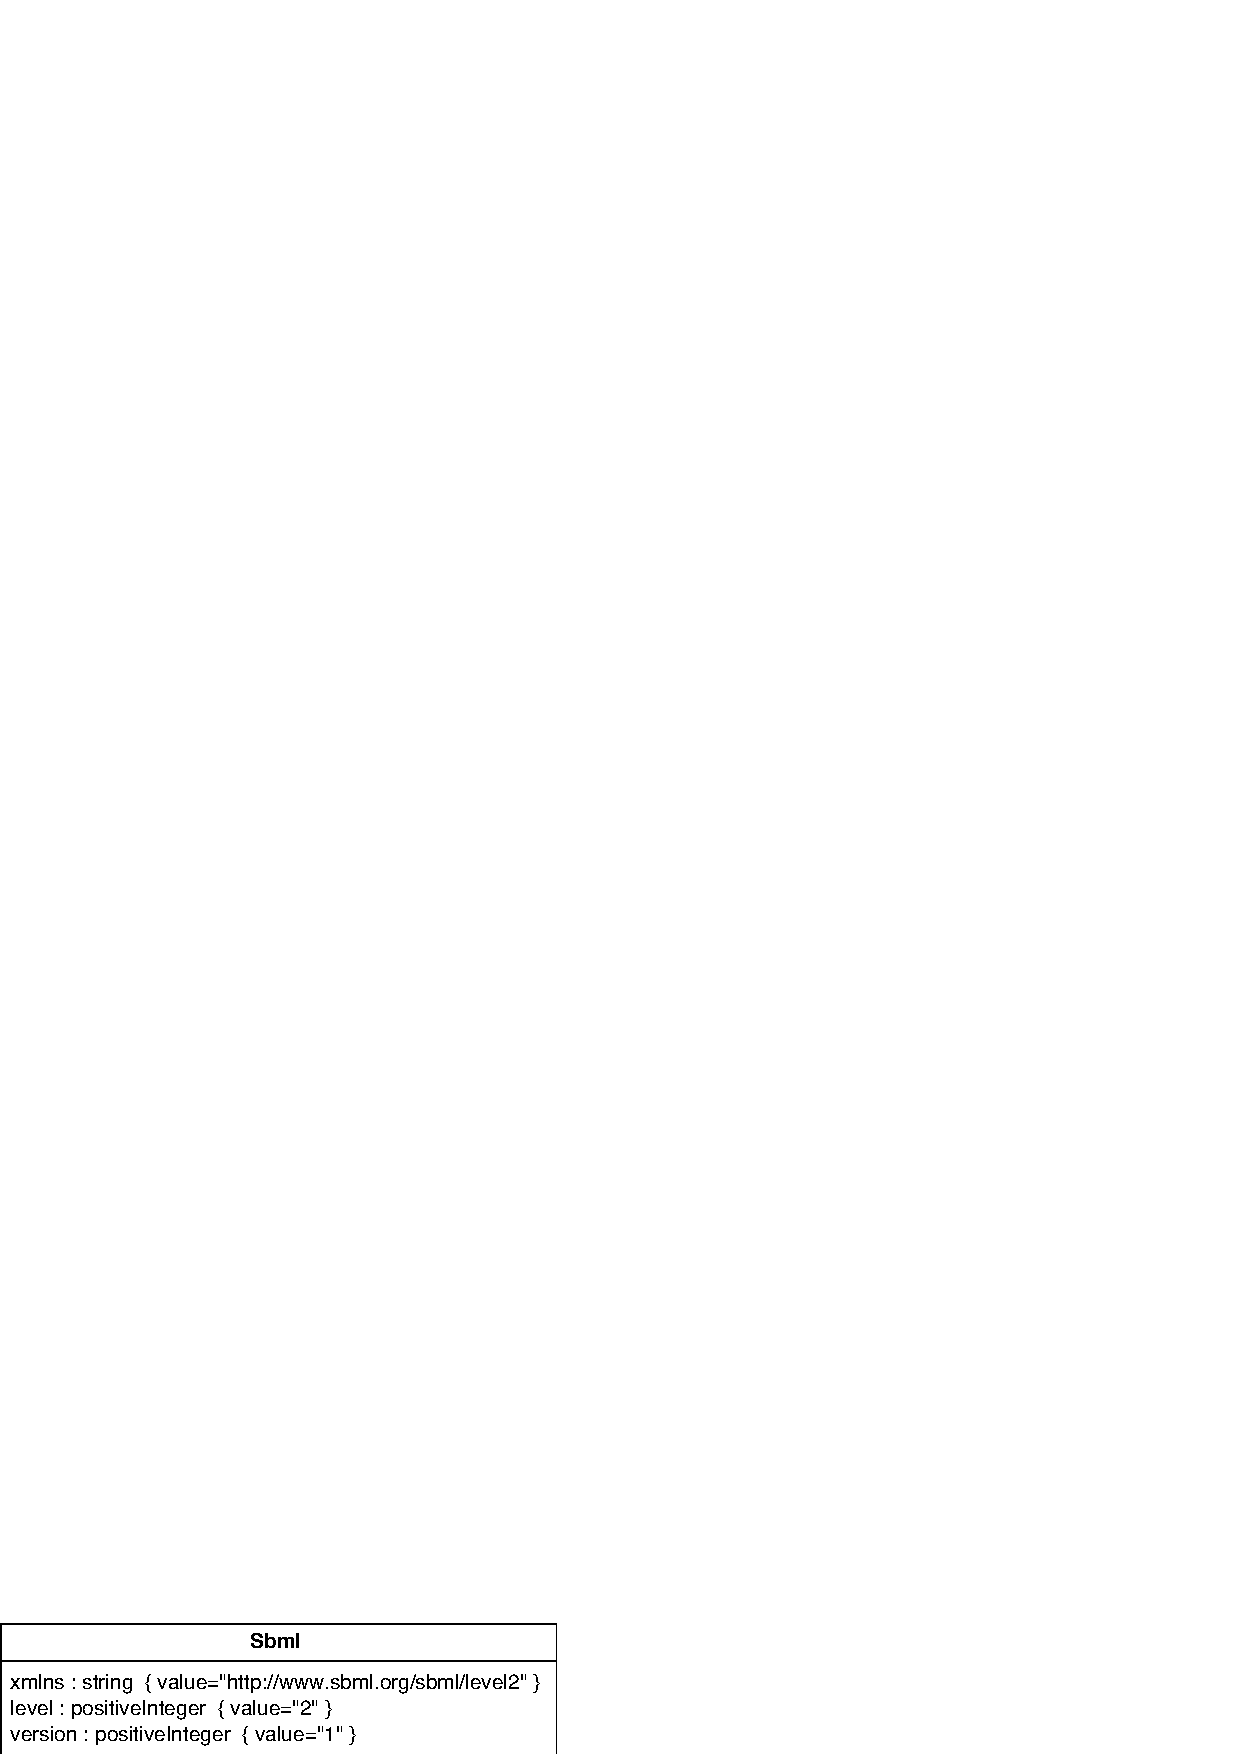
\includegraphics[scale = 0.68]{sbml}
  \caption{The definition of \class{Sbml}.  Additional fields are
    inherited from \class{SBase} but are not shown here.}
  \label{fig:sbml}
\end{figure}

The XML namespace URI for SBML Level~2 is
``\texttt{http://www.sbml.org/sbml/level2}''.  All SBML Level~2 elements
should be encoded using this URI by assigning this URI to either the
default namespace or a tag prefix.  The character encoding for SBML is
UTF-8.  SBML documents should include the \attrib{encoding} attribute with
the value \attribvalue{UTF-8} in the XML prologue.

In the transformation of UML to XML used in this document, the \class{Sbml}
structure is turned into an element named \texttt{sbml}.  The element has
two required attributes: \attrib{level} and \attrib{version}.  For SBML
Level~2 Version~1, these attributes must be set to ``\texttt{2}'' and
``\texttt{1}'', respectively.  (The \texttt{version} attribute is present
in case SBML Level~2 must be revised in the future to correct errors.)


The following is an abbreviated example of the outermost content of an SBML
model definition in XML:

\begin{example}
<?xml version="1.0" encoding="UTF-8"?>
<sbml xmlns="http://www.sbml.org/sbml/level2" level="2" version="1">
  ...
</sbml>
\end{example}


%-----------------------------------------------------------------------------
\subsection{Models}
\label{sec:model}
%-----------------------------------------------------------------------------

The \class{Model} structure is the highest-level construct in an SBML data
stream or document.  The UML definition of \class{Model} is shown in
Figure~\vref{fig:model}.  Only one component of type \class{Model} is
allowed per instance of an SBML document or data stream, although it does
not necessarily need to represent a single biological entity.

\begin{figure}[htb]
  \centering
  
\includegraphics[scale = 0.68]{model}
  \caption{The definition of \class{Model}.  Additional fields are
    inherited from \class{SBase}.}
  \label{fig:model}
\end{figure}

\class{Model} serves as a container for \class{FunctionDefinition},
\class{UnitDefinition}, \class{Compartment}, \class{Species},
\class{Parameter}, \class{Rule}, \class{Reaction} and \class{Event}
components.  All of these components are optional; that is, the lists in
each of the respective fields are permitted to have zero length.  (However,
there are dependencies between components, such that defining some requires
defining others.  For example, as explained in other sections below,
defining a species requires defining a compartment, and defining a reaction
requires defining a species.)

The \class{Model} structure has an optional field, \attrib{id}, used to
give the model an identifier.  The identifier must be a text string
conforming to the syntax permitted by the \class{SId} data type described
in Section~\ref{sec:id}.  \class{Model} also has an optional \attrib{name}
field, of type \class{string}.  The \attrib{name} and \attrib{id} fields
should be used as described in Section~\ref{sec:idnameattribs}.

In the XML encoding of an SBML model, the lists of species, compartments,
unit definitions, parameters, reactions, function definitions, rules and
events are translated into lists of XML elements enclosed within elements
of the form \class{listOf}\rule{0.5in}{0.5pt}\class{s}, where the blank is
replaced by the name of the component type (e.g., ``\texttt{Reaction}'').
The resulting XML data object has the form illustrated by the following
skeletal model:

\begin{example}
<model id="My_Model">
    <listOfFunctionDefinitions>
        ...
    </listOfFunctionDefintions>
    <listOfUnitDefinitions>
        ...
    </listOfUnitDefinitions>
    <listOfCompartments>
        ...
    </listOfCompartments>
    <listOfSpecies>
        ...
    </listOfSpecies>
    <listOfParameters>
        ...
    </listOfParameters>
    <listOfRules>
        ...
    </listOfRules>
    <listOfReactions>
        ...
    </listOfReactions>
    <listOfEvents>
        ...
    </listOfEvents>
</model>
\end{example}

Readers may wonder about the motivations for the
\class{listOf}\rule{0.5in}{0.5pt}\class{s} notation.  A simpler approach to
creating the lists of components would be to place them all directly
at the top level under \texttt{<model> ... </model>}.  We chose instead to
group them within XML elements named after
\class{listOf}\rule{0.5in}{0.5pt}\class{s}, because we believe this helps
organize the components and makes visual reading of model definitions
easier.  These \class{listOf}\rule{0.5in}{0.5pt} elements are derived from
\class{SBase} which enables each list to contain its own \attrib{metaid},
\attrib{notes} and \attrib{annotation} fields.
Further details of how \class{listOf}\rule{0.5in}{0.5pt} elements
implement UML lists is described in Appendix~\ref{apdx:notation}.

%-----------------------------------------------------------------------------
\subsection{Function Definitions}
\label{sec:functions}
%-----------------------------------------------------------------------------

The \class{FunctionDefinition} structure associates an identifier with a
function definition.  The identifier can then be used in any subsequent
MathML \class{apply} elements.  \class{FunctionDefinition} is shown in
Figure~\ref{fig:mathdefinition}.

\begin{figure}[htb]
  \centering
  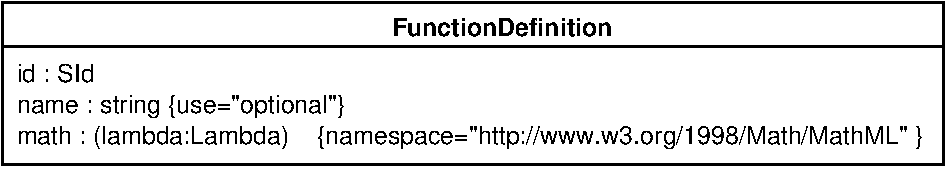
\includegraphics[scale = 0.68]{mathdefinition}
  \caption{The definition of \class{FunctionDefinition}.  Fields inherited
  from \class{SBase} are omitted here but are assumed.}
  \label{fig:mathdefinition}
\end{figure}

The \class{FunctionDefinition} structure has three fields, \attrib{id},
\attrib{name} and \attrib{math}.

\subsubsection{The \attrib{id} and \attrib{name} fields}

The \attrib{id} and \attrib{name} fields
have types \class{SId} and \class{string}, respectively, and operate in the
manner described in Section~\ref{sec:idnameattribs}.  MathML \texttt{ci}
elements can refer to the function defined by a \class{FunctionDefinition}
using the value of its \attrib{id} field.

\subsubsection{The \attrib{math} field} 

The \attrib{math} field is a container for MathML content that defines the
function.  The content of this field can only be a MathML \texttt{lambda}
element.  This is the only place in SBML where a \texttt{lambda} element can
be used.  The function is only available for use in other MathML elements
that follow the \class{FunctionDefinition} structure in an SBML model.  (These
restrictions prevent recursive and mutually-recursive functions from
being expressed.)  The \texttt{lambda} element can contain any
of the elements in the MathML subset listed in Section~\ref{sec:mathmlsubset} but
not any further \texttt{lamdba} elements.

The following abbreviated SBML example shows a \class{FunctionDefinition}
structure defining $pow3(x)$ as representing $x^{3}$:

\begin{example}
<model>
    ...
    <functionDefinition id="pow3">
        <math xmlns="http://www.w3.org/1998/Math/MathML">
            <lambda>
                <bvar><ci> x </ci></bvar>
                <apply>
                    <power/>
                    <ci> x </ci>
                    <cn> 3 </cn>
                </apply>
            </lambda>
        </math>
    </functionDefinition>
    ...
</model>
\end{example}

%-----------------------------------------------------------------------------
\subsection{Unit Definitions}
\label{sec:unitdefinitions}
%-----------------------------------------------------------------------------

Units may be supplied in a number of contexts in an SBML model. The units
of the following mathematical entities can be specified explicitly: constants,
initial conditions, symbols in formulae and the results of formulae.
Rather than having to give a complete unit definition
on every structure SBML provides a facility
for defining identified units which can be reused throughout a model.
In addition by default mathematical entities have units composed from
built-in units in a consistent fashion (see Sections~\ref{sec:built-in-units},
\ref{sec:compartment-units}, \ref{sec:species-units} and~\ref{subsec:kinetic-law}).
By redefining the built-in units it is possible to change the units
used throughout a model in a simple and consistent manner.  
The SBML \class{UnitDefinition}  and
\class{Unit} structures enable combinations of units to
be given abbreviated names and enables built-in units to be redefined.
The definitions of \class{UnitDefinition}  and
\class{Unit} are shown in
Figure~\vref{fig:unitdefinition}.

\begin{figure}[htb]
  \vspace*{8pt}
  \centering
  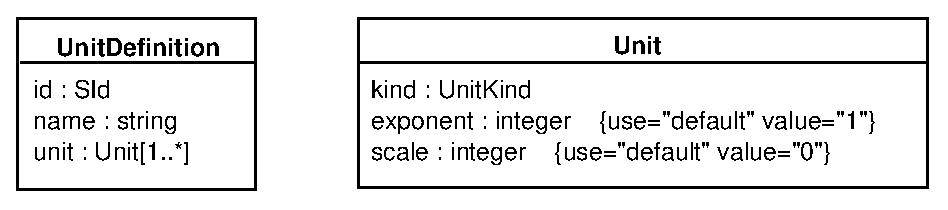
\includegraphics[scale = 0.68]{unitdefinition}
  \caption{The definition of \class{UnitDefinition} and \class{Unit}.}
  \label{fig:unitdefinition}
\end{figure}

\subsubsection{The \class{UnitDefinition} structure}

An instance of a \class{UnitDefinition} consists of an \attrib{id} field of
type \class{SId}, an optional string field \attrib{name} and an optional
list of structures of type \class{Unit}.  As mentioned in
Section~\ref{sec:namespaces}, unit identifiers defined by the \attrib{id}
field are considered to be in a separate global namespace distinct from the
namespace of other identifiers in a model; thus, unit identifiers cannot collide
with the identifiers of species, compartments, reactions etc.
The approach to defining units in SBML is compositional; for example,
$meter\ second^{\,-2}$ is constructed by combining, within the same
\class{UnitDefinition} \class{Unit} list, a \class{Unit} structure representing
$meter$ with a \class{Unit} structure representing $second^{\,-2}$.

\subsubsection{The \class{Unit} structure}

The \class{Unit} data structure has one required field,
\attrib{kind}, whose value must be taken from \class{UnitKind}, an
enumeration of base units.  The possible values of \class{UnitKind} are given in
Table~\vref{tab:unitkind}.

\begin{table}[bh]
  \centering
  \vspace*{12pt}                        % SPECIFIC ADJUSTMENT FOR THIS PAGE
  \ttfamily
  \begin{tabular}{llllll}
    \toprule
    ampere      & farad & joule     & lux       & radian   & volt   \\
    becquerel   & gram  & katal     & metre     & second   & watt\\
    candela     & gray  & kelvin    & mole      & siemens  & weber\\
    Celsius     & henry & kilogram  & newton    & sievert\\
    coulomb     & hertz & litre     & ohm       & steradian\\
    \underline{dimensionless} & \underline{item} & lumen     & pascal    & tesla\\
    \bottomrule
  \end{tabular}
  \caption{The possible values of \attrib{kind} in a \class{UnitKind}
    structure.  All are names of base or derived SI
    units~\protect\citep{bipm:2000}, except for
    ``\texttt{dimensionless}'' and ``\texttt{item}'', which are 
    SBML additions important for handling certain common situations.
    ``\texttt{Dimensionless}'' is intended for cases where a quantity does not
    have units, and ``\texttt{item}'' for expressing
    such things as ``N items'' (e.g., ``100 molecules'').
    Although ``\texttt{Celsius}'' is capitalized, for 
    simplicity, SBML
    requires that these unit names be treated in a case-insensitive manner.
    Also, note that the gram and litre are not
    strictly part of SI; however, they are so
    commonly used in SBML's areas of application that they 
    are included as predefined unit names.  (The standard SI unit of
    mass is in fact the kilogram, and volume is
    defined in terms of cubic meters.)}
  \label{tab:unitkind}
\end{table}

Note that the set of acceptable values for the field \attrib{kind} does not
include units defined by \class{UnitDefinition} structures.  This
means that the units definition feature in SBML is not
hierarchial---user-defined units cannot be built on top of other
user-defined units, only on top of base units.  SBML differs from CellML in
this respect; CellML does allow the construction of hierarchial unit
definitions.

An instance of a \class{Unit} definition represents a (possibly
transformed) reference to a base unit chosen from \class{UnitKind}.  The
formula for a single transformation represented by \class{Unit} definition
is as follows (where $u$ is the original base unit and $u_\emph{new}$ is
the new unit):
\begin{equation*}
  u_\emph{new} = (\emph{multiplier} \times 10^\emph{scale} 
  \times u^\emph{exponent}) + \emph{offset}
\end{equation*}
The optional \attrib{exponent} field on \class{Unit} represents an exponent
on the unit.  Its default value is ``\attribvalue{1}'' (one).  For the
example mentioned at the beginning of this section, $second^{\,-2}$ would
be obtained by using \texttt{kind="second"} and \texttt{exponent="-2"}.  A
\class{Unit} structure also has an optional \attrib{scale} field; its value
must be an integer exponent for a power of ten multiplier used to set the
scale of the unit.  For example, a unit that has a \attrib{kind} value of
``\attribvalue{gram}'' and a \attrib{scale} value of ``\attribvalue{-3}''
signifies $10^{-3} * gram$, or milligrams.  The default value of
\texttt{scale} is ``\attribvalue{0}'' (zero), because $10^0 = 1$.

The optional \attrib{multiplier} field can be used to multiply the
\attrib{kind} unit by a real-numbered factor; this enables the definition
of units that are not power-of-ten multiples of SI units.  For instance, a
\attrib{multiplier} of 0.3048 could be used to define ``foot'' as a measure
of length in terms of a metre.  The \attrib{multiplier} field has a default
value of ``\attribvalue{1}'' (one).  Finally, the \attrib{offset} field is
used to represent the addition of a constant in the transformation the
\attrib{kind} unit.  For example, an \attrib{offset} value of
``\attribvalue{32.0}'' would be needed to define Fahrenheit in terms of
degrees Celsius.  The \attrib{offset} field has a default value of
``\attribvalue{0}'' (zero).

The composition of $n$ \class{Unit} structures within a
\class{UnitDefinition} to create more complex units involves a linear
product according to the following formula:
\begin{equation*}
  u_\emph{new} = m_1 \times \ldots \times m_n
  \times 10^{s_1} \times \ldots \times 10^{s_n} 
  \times u^{e_1} \times \ldots \times u^{e_n}
\end{equation*}

The following example illustrates the definition of an abbreviation named
``\unit{mmls}'' for the units $mmol\ l^{-1}\ s^{-1}$:

\begin{example}
<listOfUnitDefinitions>
    <unitDefinition id="mmls">
        <listOfUnits>
            <unit kind="mole"   scale="-3"/>
            <unit kind="litre"  exponent="-1"/>
            <unit kind="second" exponent="-1"/>
        </listOfUnits>
    </unitDefinition>
</listOfUnitDefinitions>
\end{example}

The following example defines Fahrenheit:

\begin{example}
<unitDefinition id="Fahrenheit">
     <listOfUnits>
         <unit kind="Celsius" multiplier="1.8" offset="32"/>
     </listOfUnits>
</unitDefinition>
\end{example}

\subsubsection{Built-in Units}
\label{sec:built-in-units}

There are five special unit names in SBML, listed in
Table~\vref{tab:builtin}, corresponding to the five types of quantities or
\emph{built-in units} that play roles in biochemical reactions: amount of
substance, volume, area, length and time.  
By default these units either composed or used directly to define the
units of all SBML math entities apart from parameters.
SBML defines defaults for the
built-in units, see the 3rd column of Table~\ref{tab:builtin}, all with
default \texttt{scale} and \texttt{offset} values of zero and default
\texttt{multiplier} values of one.

\begin{table}[htb]
  \centering
  \small
  \setlength{\tabcolsep}{4.5pt}
  \begin{tabular}{lll>{\ttfamily}l}
    \toprule
    \textbf{Name} & \textbf{Possible Scalable Units} & \textbf{Default Units}\\
    \midrule
    \unit{substance} & mole, item & mole\\
    \unit{volume} & litre, cubic metre & litre\\
    \unit{area}   & square metre & square metre\\
    \unit{length} & metre & metre\\
    \unit{time}   & second & second\\
    \bottomrule
  \end{tabular}
  \caption{SBML's built-in units.}
  \label{tab:builtin}
\end{table}

A field on a structure, such as \attrib{units} on \class{Parameter}, which
defines the units for that mathematical entity can refer to one of several
named units:
\begin{itemize}
\item the predefined units from Table~\vref{tab:unitkind},
\item new units defined in unit definitions, or
\item the five predefined names of built-in units ``\unit{substance}'', ``\unit{volume}'',
``\unit{area}'', ``\unit{length}'', and ``\unit{time}'' from
Table~\ref{tab:builtin}.
\end{itemize}

Within certain limits, a model may change the built-in units by reassigning
the keywords ``\unit{substance}'', ``\unit{length}'', ``\unit{area}'',
``\unit{time}'', and ``\unit{volume}'' in a \class{UnitDefinition}.  The
second column in Table~\ref{tab:builtin} lists the set of units that should be
used in redefining a given built-in unit.  

The following example illustrates how to change the built-in units of volume
to be milliliters.  If this definition appeared in a model, the units of
volume on all components that did not explicitly specify different units
would be changed to milliliters.
\begin{example}
<model>
    ...
    <listOfUnitDefinitions>
        <unitDefinition id="volume">
            <listOfUnits>
                <unit kind="liters" scale="-3"/>
            </listOfUnits>
        </unitDefinition>
    </listOfUnitDefinitions>
    ...
</model>
\end{example}

Software developers are asked to pay special attention to the units used in
an SBML model.  Different users and developers sometimes make different
assumptions about units, and these assumptions may not correspond to what
is defined in SBML.  Sections~\ref{sec:ci-token}, \ref{sec:species-units} and
\ref{subsec:kinetic-law} have particularly important notes about the usage
of units in SBML.


%-----------------------------------------------------------------------------
\subsection{Compartments}
\label{sec:compartments}
%-----------------------------------------------------------------------------

A \emph{compartment} in SBML represents a bounded space in which species
are located.  Compartments do not necessarily have to correspond to actual
structures inside or outside of a cell, although models are often designed
that way.  The definition of \class{Compartment} is shown in
Figure~\vref{fig:compartment}.

\begin{figure}[htb]
  \vspace*{8pt}
  \centering
  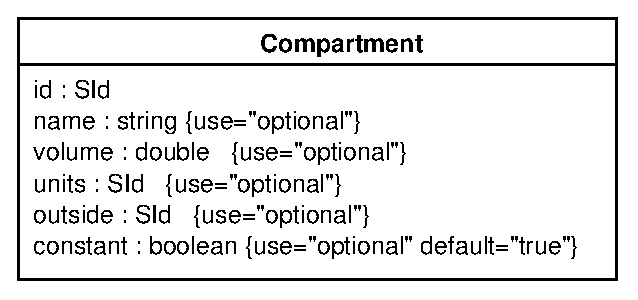
\includegraphics[scale = 0.68]{compartment}
  \caption{The definition of \class{Compartment}.
    Fields inherited from \class{SBase} are omitted here but are assumed.}
  \label{fig:compartment}
\end{figure}

It is worth pointing out that, although compartments are optional in the
overall definition of \class{Model} (see Section~\ref{sec:model}), every
species in an SBML model must be located in a compartment.  This in turn
means that if a model declares any species, that model must also declare at
least one compartment.

\subsubsection{The \attrib{id} and \attrib{name} Fields}

\class{Compartment} has one required field, \attrib{id}, of type
\class{SId}, to give the compartment a unique identifier by which other
parts of an SBML model definition can refer to it.  A compartment can also
have an optional \attrib{name} field of type \class{string}.  Identifiers
and names should be used according to the guidelines described in
Section~\ref{sec:idnameattribs}.

\subsubsection{The \attrib{spatialDimensions} Field}

A \class{Compartment} structure has an optional field
\attrib{spatialDimensions}, whose value must be a positive integer
indicating the number of spatial dimensions possessed by the compartment.
The maximum value of \attrib{spatialDimensions} is ``\texttt{3}'', meaning
a three-dimensional structure (a volume).  Other permissible values are
``\texttt{2}'' (for a two-dimensional area), ``\texttt{1}'' (for a
one-dimensional curve), and ``\texttt{0}'' (for a point).  The default value
is ``\texttt{3}''.

\subsubsection{The \attrib{size} Field}
\label{sec:size}

Each compartment has an optional floating-point field named
\attrib{size}, representing the total size of the compartment.  The
\attrib{size} field enables concentrations of species to be calculated in
the absence of geometry information.  Note in particular that in SBML Level~2,
a missing \attrib{size} value does \emph{not} imply that the compartment size is 1.
(This is unlike the definition of compartment \attrib{volume} in SBML
Level~1.).  The \attrib{size} field must not be present if the
\attrib{spatialDimensions} field is has value ``\texttt{0}''.
When \attrib{spatialDimensions} field doesn't have value ``\texttt{0}''
a missing value for \attrib{size} for a given compartment signifies that the value is
either unknown, is determined by an assignment rule, not required for analysis,
or available from an external data source.  

\subsubsection{The \attrib{units} Field}
\label{sec:compartment-units}

The units associated with the compartment's \attrib{size} value may be
explicitly set using the optional field \attrib{units}.  The value chosen
for this field must be either one of the base units from
Table~\vref{tab:unitkind}, or the built-in units ``\unit{volume}'',
``\unit{area}'', ``\unit{length}'' or ``\unit{dimensionless}'', or a new
unit defined by a unit definition in the enclosing model.  The type of
units assigned to the \attrib{units} field must also agree with the number
of spatial dimensions of the compartment; that is, they must be units of
volume if the value of \attrib{spatialDimensions} is ``\attribvalue{3}'';
they must be units of area if the value of \attrib{spatialDimensions} is
``\attribvalue{2}''; they must be units of length if the value of
\attrib{spatialDimensions} is ``\attribvalue{1}''; and they must be
``\unit{dimensionless}'' if the value of \attrib{spatialDimensions} is
``\attribvalue{0}''.  The default units depends on the value of the
compartment's \attrib{spatialDimensions} attribute according to the
following rule: for spatial dimensions of 3, 2, 1 or 0, the
compartment has the default units of \unit{volume}, \unit{area},
\unit{length} and \unit{dimensionless}, respectively.  (See
Table~\vref{tab:builtin} and Table~\vref{tab:unitkind}.)

The units of the compartment size, as defined by the \attrib{units} attribute,
are used as in the following ways.
\begin{itemize}

\item The value of the \attrib{units} field is used as the units of the \attrib{size}
  field of the 
  compartment structure (see Section~\ref{sec:size}). 

\item The value of the \attrib{units} field is used as the units of the 
  compartment identifier when it appears as a numerical quantity in a mathematical
  formula expressed in MathML (discussed in Section~\ref{sec:ci-token}).

\item The value of the \attrib{units} field is used as the units of the 
  \attrib{math} field of the
  \class{AssignmentRule} structures determining the compartment's size
  (see Section~\ref{sec:assignmentrule}).

\item In \class{RateRule} structures that
  set the rate of change of the compartment's size
  (Section~\ref{sec:raterule}), the units on the rule's \attrib{math} field are
  those in the compartment's \attrib{units} field divided by the default
  \quantity{time} units.  (In other words, the units for the rate of change
  of compartment size are \quantity{compartment size}/\quantity{time} units.)
\end{itemize}

\subsubsection{The \attrib{constant} Field}

A \class{Compartment} also has an optional boolean field called
\attrib{constant} which indicates whether the compartment's size stays
constant or can vary during a simulation.  A value of
``\attribvalue{false}'' indicates that the compartment's size can be
determined by rules (see Section~\ref{sec:rules}), and the value of the
\attrib{size} field should be taken as being the initial size of the
compartment.  The default value for the \attrib{constant} field is
``\attribvalue{true}'' because in the most common modeling scenarios at
the time of this writing, compartment sizes remain constant.
The \attrib{constant} field must default to or be set to ``\attribvalue{true}''
if the \attrib{spatialDimensions} field is 0.

\subsubsection{The \attrib{outside} Field}

The optional field \attrib{outside} of type \class{SId} can be used to
express containment relationships between compartments.  If present, the
value of \attrib{outside} for a given compartment must be the name of
another compartment enclosing it, or in other words, the compartment that
is ``outside'' of it.  This enables the representation of simple
topological relationships between compartments, for those simulation
systems that can make use of the information (e.g., for drawing simple
diagrams of compartments).

Although containment relationships are partly taken into account by the
compartmental localization of reactants and products, it is not always
possible to determine purely from the reaction equations whether one
compartment is meant to be located within another.  In the absence of a
value for \attrib{outside}, compartment definitions in SBML Level~2 do not
have any implied spatial relationships between each other.  For many
modeling applications, the transfer of substances described by the
reactions in a model sufficiently express the relationships between the
compartments.  (As discussed in Section~\ref{sec:level-3}, we expect that
SBML Level~3 will introduce the ability to define geometries and spatial
qualities.)

\subsubsection{Examples}

The following example illustrates two
compartments in an abbreviated SBML example of a model definition:
\begin{example}
<model>
    ...
    <listOfCompartments>
        <compartment id="cytosol" size="2.5"/>
        <compartment id="mitochondria" size="0.3"/>
    </listOfCompartments>
    ...
</model>
\end{example}

The following is an example of using \attrib{outside} to model a cell
membrane.  To express that a compartment named B has a membrane that is
modeled as another compartment M, which in turn is located within another
compartment A, one would write:
\begin{example}
<model>
    ...
    <listOfCompartments>
        <compartment id="A"/>
        <compartment id="M" spatialDimensions="2" outside="A"/>
        <compartment id="B" outside="M"/>
    </listOfCompartments>
    ...
</model>
\end{example}

%-----------------------------------------------------------------------------
\subsection{Species}
\label{sec:species}
%-----------------------------------------------------------------------------

The term \emph{species} refers to chemical entities that take part in
reactions.  These include simple ions (e.g., protons, calcium), simple
molecules (e.g., glucose, ATP), large molecules (e.g., RNA,
polysaccharides, and proteins), and others.  The \class{Species} data
structure is intended to represent these entities.  Its definition is shown
in Figure~\vref{fig:species}.

\begin{figure}[htb]
  \centering
  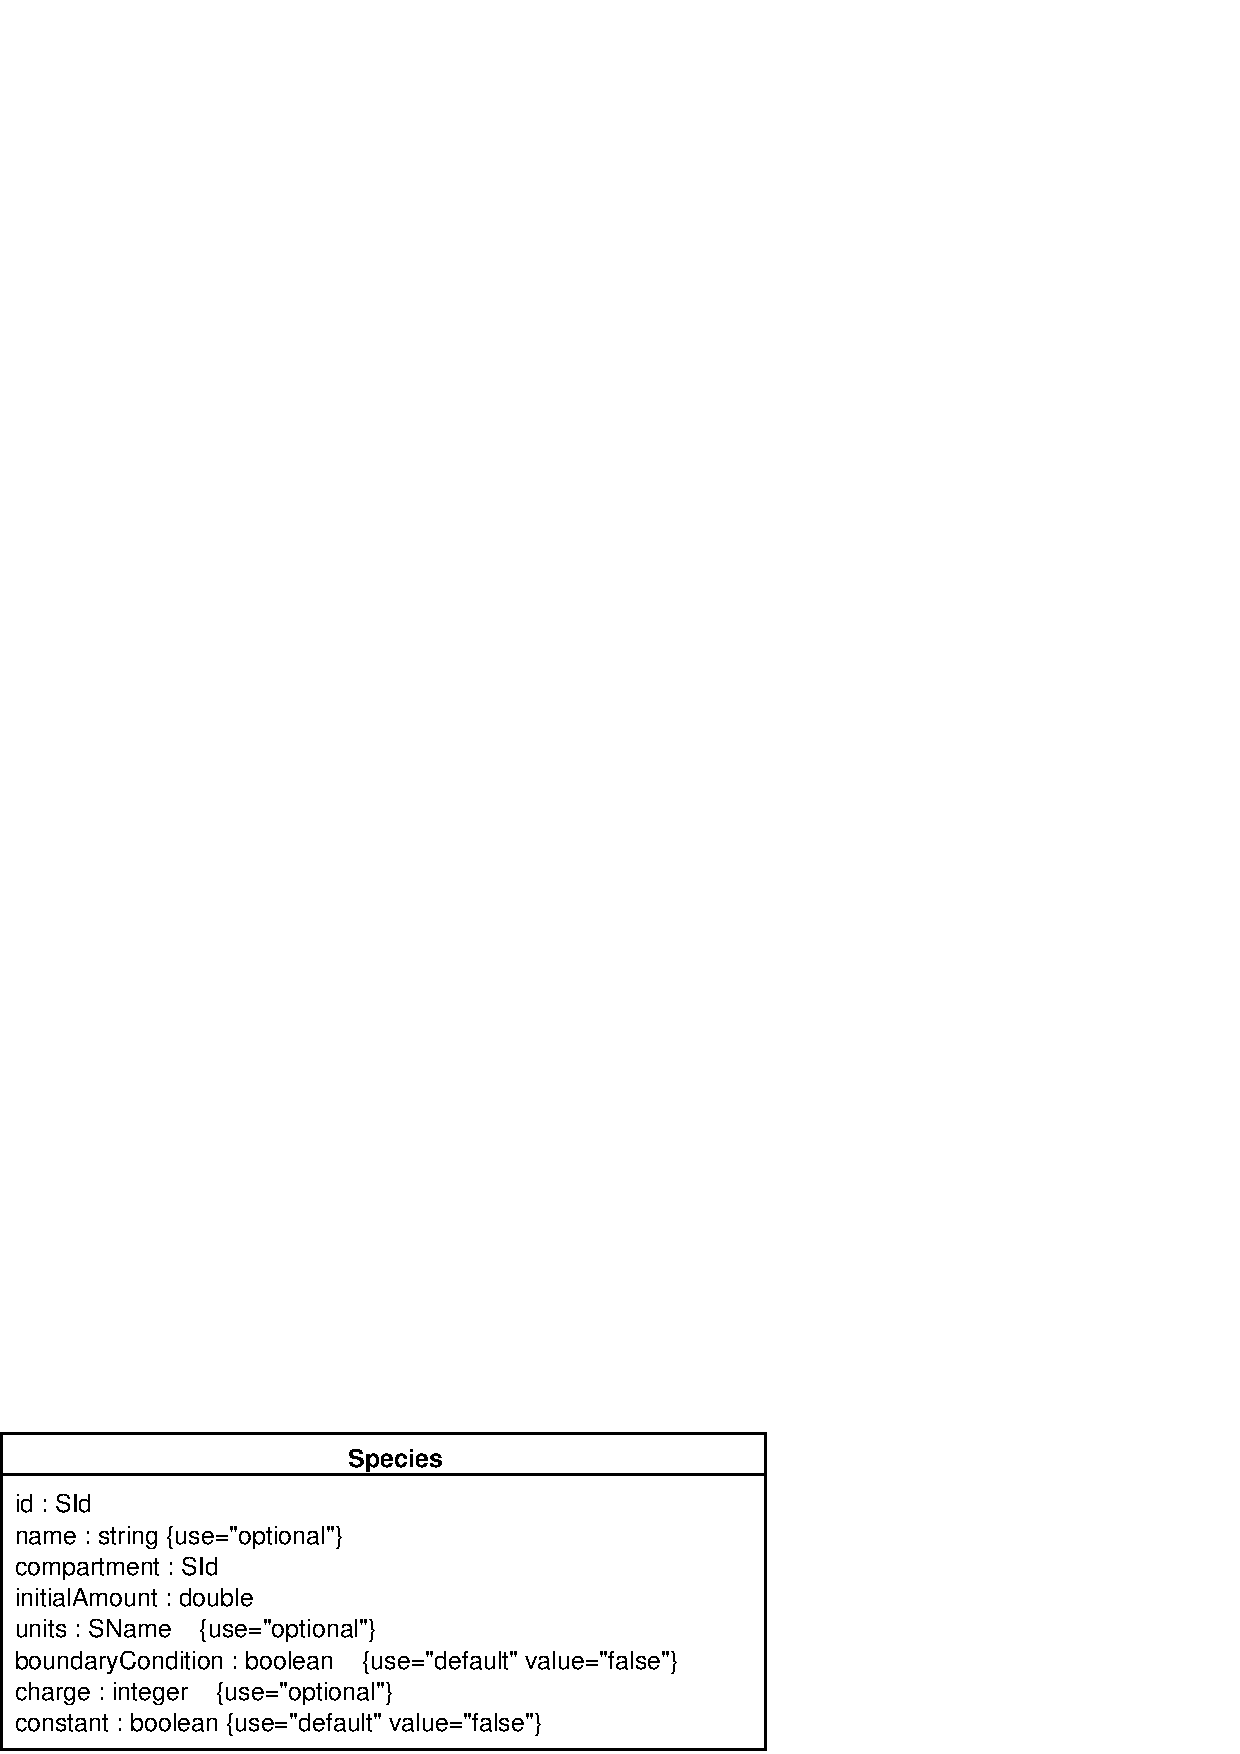
\includegraphics[scale = 0.68]{specie}
  \caption{The definition of \class{Species}.  As usual, fields inherited from
    \class{SBase} are omitted here but are assumed.}
  \label{fig:species}
\end{figure}

\subsubsection{The \attrib{id} and \attrib{name} attributes}

As with other major structures in SBML, \class{Species} has an mandatory
field, \attrib{id}, used to give the species an identifier.  The identifier
must be a text string conforming to the syntax permitted by the \class{SId}
data type described in Section~\ref{sec:id}.  \class{Species} also has an
optional \attrib{name} field, of type \class{string}.  The \attrib{name}
and \attrib{id} fields should be used as described in
Section~\ref{sec:idnameattribs}.

\subsubsection{The \attrib{compartment} Field}

The required field
\attrib{compartment}, also of type \class{SId}, is used to identify the
compartment in which the species is located.  The field's value must be the
identifier of an existing \class{Compartment} structure.  It is important
to note that there is no default value for the \attrib{compartment} field
on \class{Species}: every species in an SBML model must be assigned a
compartment, and consequently, a model must define at least one compartment
if that model contains any species.

\subsubsection{The \attrib{initialAmount} and \attrib{initialConcentration} Fields}
\label{sec:initialAmount}

The optional fields \attrib{initialAmount} and
\attrib{initialConcentration}, both having a data type of \class{double},
are used to set the initial quantity of the species in the named
compartment.  These fields are mutually exclusive i.e. \emph{only one} can
have a value on any given instance of a \class{Species} structure.  Also,
\attrib{initialConcentration} must not have a value if the species'
compartment has a \attrib{spatialDimensions} value of ``\texttt{0}''.  (The
reason is simply that there cannot be a concentration defined when the
compartment has no spatial extent.)  Missing \attrib{initialAmount} or
\attrib{initialConcentration} values implies that their values are either
unknown, set by an assignment rule, not required for analysis or available from
an external data source.

The units of the value in the \attrib{initialAmount} field is that given by
the \attrib{substanceUnits} field of the species structure.  The units of the value
in the \attrib{initialConcentration} field are the \emph{units of the species}
see Section~\ref{sec:species-units}.

\subsubsection{The \attrib{substanceUnits} and \attrib{spatialSizeUnits} Fields}
\label{sec:species-units}

The units associated with species, referred to as the \emph{units of the species},
are determined via the
optional fields \attrib{substanceUnits} and \attrib{spatialSizeUnits}.
The \emph{units of the species} can be thought of as the concentration
units of the species if one adopts a broad definition of concentration.
The \emph{units of the species} are of the form
\quantity{substance}/\quantity{size} units if the compartment's
\attrib{spatialDimensions} are non-zero or are of the form \quantity{substance} if 
\attrib{spatialDimensions} are zero.
The units of
\quantity{substance} are those defined in the \attrib{substanceUnits}, and
the \quantity{size} units are those given
in the \attrib{spatialSizeUnits} attribute.

In the case of both \attrib{substanceUnits} and \attrib{spatialSizeUnits} fields
the value chosen must be either
a base unit from Table~\vref{tab:unitkind}, a built-in unit from
Table~\vref{tab:builtin},
or a new unit defined by a unit definition in the enclosing model.
The chosen
units for \attrib{substanceUnits} must be a variant of
\unit{mole} or \unit{item} units.
The \attrib{substanceUnits} field defaults to the
the built-in unit ``\attrib{substance}'' shown in
Table~\vref{tab:builtin}.

The type of
units assigned to the \attrib{spatialSizeUnits} field must agree with the number
of spatial dimensions of the species' compartment; that is, they must be units of
volume if the value of the compartment's \attrib{spatialDimensions} is
``\attribvalue{3}'';
they must be units of area if the value of \attrib{spatialDimensions} is
``\attribvalue{2}''; and they must be units of length if the value of
\attrib{spatialDimensions} is ``\attribvalue{1}''.
The \attrib{spatialSizeUnits} must not have a value if the value of
\attrib{spatialDimensions} is ``\texttt{0}''.
The default value of the \attrib{spatialSizeUnits} is the value of
the \attrib{units} field of the species' compartment.

The \emph{units of the species} are used in the
following ways.

\begin{itemize}

\item The species \attrib{initialConcentration} field has these units.
  (see Section~\ref{sec:initialAmount}).

\item The 
  species identifier has these units when it appears as a numerical quantity
  in a mathematical formula expressed in MathML
  (discussed in Section~\ref{sec:ci-token}).

\item The
   \attrib{math} field of the
  class{AssignmentRule} structures determining the species' concentration
  (see Section~\ref{sec:assignmentrule}) has these units.

\item In \class{RateRule} structures that
  set the rate of change of the species' concentration
  (Section~\ref{sec:raterule}), the units on the rule's \attrib{math} field are
  the \emph{units of the species} divided by the built-in
  \quantity{time} units.

\end{itemize}


\subsubsection{The \attrib{constant} and \attrib{boundaryCondition} Fields}

The \class{Species} structure has optional boolean field named
\attrib{constant} which is used to indicate whether the concentration of
that species can vary during a simulation.  The default value is
``\attribvalue{false}'', indicating that the species' concentration can be
determined by rules and reactions.

Another optional field defined for \class{Species} is
\attrib{boundaryCondition}.  By default, when a species is a product or
reactant of one or more reactions, its concentration is determined by those
reactions.  In SBML, it is possible to indicate that a given species'
concentration is \emph{not} determined by the set of reactions even when
that species occurs as a product or reactant; i.e., the species is on the
\emph{boundary} of the reaction system but is a component of the rest of
the model.  The boolean field \attrib{boundaryCondition} can be used to
indicate this.  The value of the field defaults to ``\attribvalue{false}'',
indicating that by default, the species \emph{is} part of the reaction
system.  Table~\ref{tab:specieattrib} shows how to interpret the combined
values of the \attrib{boundaryCondition} and \attrib{constant} fields.  In
practice, a \attrib{boundaryCondition} value of ``\attribvalue{true}''
means that a differential equation derived from the reaction definitions
should not be generated for the species.  The example model in
section~\ref{sec:constantspecieseg} contains all four possible combinations
of the \attrib{boundaryCondition} and \attrib{constant} attributes on
\class{species} elements.  Section~\ref{sec:odeeg} contains a translation into
ODEs of a model which uses \attrib{boundaryCondition} and \attrib{constant}
attributes.

\begin{table}[ht]
  \vspace*{10pt}
  \centering
  \begin{tabular}{lllll}
    \toprule
    \textbf{\attrib{constant}} & \textbf{\attrib{boundaryCondition}} &
    \textbf{can have} & \textbf{can be} & \textbf{concentration} \\
    \textbf{value} & \textbf{value} & \textbf{assignment} & \textbf{reactant or} & \textbf{is changed by} \\
    & & \textbf{or rate rule} & \textbf{product}\\
    \midrule
    true & true & no & yes & never changes\\
    false & true & yes & yes & rule \\
    true & false & no & no & never changes \\
    false & false & yes & yes & reactions or rule but not both \\
    \bottomrule
  \end{tabular}
  \caption{How to interpret the values of the \attrib{constant} and
    \attrib{boundaryCondition} fields of the \class{Species} structure.}
  \label{tab:specieattrib}
\end{table}

\subsubsection{The \attrib{charge} Field}

Finally, the optional field \attrib{charge} on \class{Species} takes an
integer indicating the charge on the species (in terms of electrons, not
the SI unit Coulombs). This may be useful when the species involved is a
charged ion such as calcium ($\text{Ca}^{2+}$).

\subsubsection{Example}

The following example shows two species definitions within an
abbreviated SBML model definition.  The example shows that species
are listed under the heading \attrib{listOfSpecies} in the model:

\begin{example}
<model>
    ...
    <listOfSpecies>
        <species id="Glucose" compartment="cell" initialConcentration="4"/>
        <species id="Glucose_6_P" compartment="cell" initialConcentration="0.75"/>
    </listOfSpecies>
    ...
</model>

\end{example}


%-----------------------------------------------------------------------------
\subsection{Parameters}
\label{sec:parameters}
%-----------------------------------------------------------------------------

A \class{Parameter} structure is used to declare a variable for use in
mathematical formulas in an SBML model definition.  By default, parameters
have constant value for the duration of a simulation and for this reason
are called ``parameters'' instead of variables in SBML.  The definition of
\class{Parameter} is shown in Figure~\vref{fig:parameter}.

\begin{figure}[htb]
  \vspace*{12pt}
  \centering
  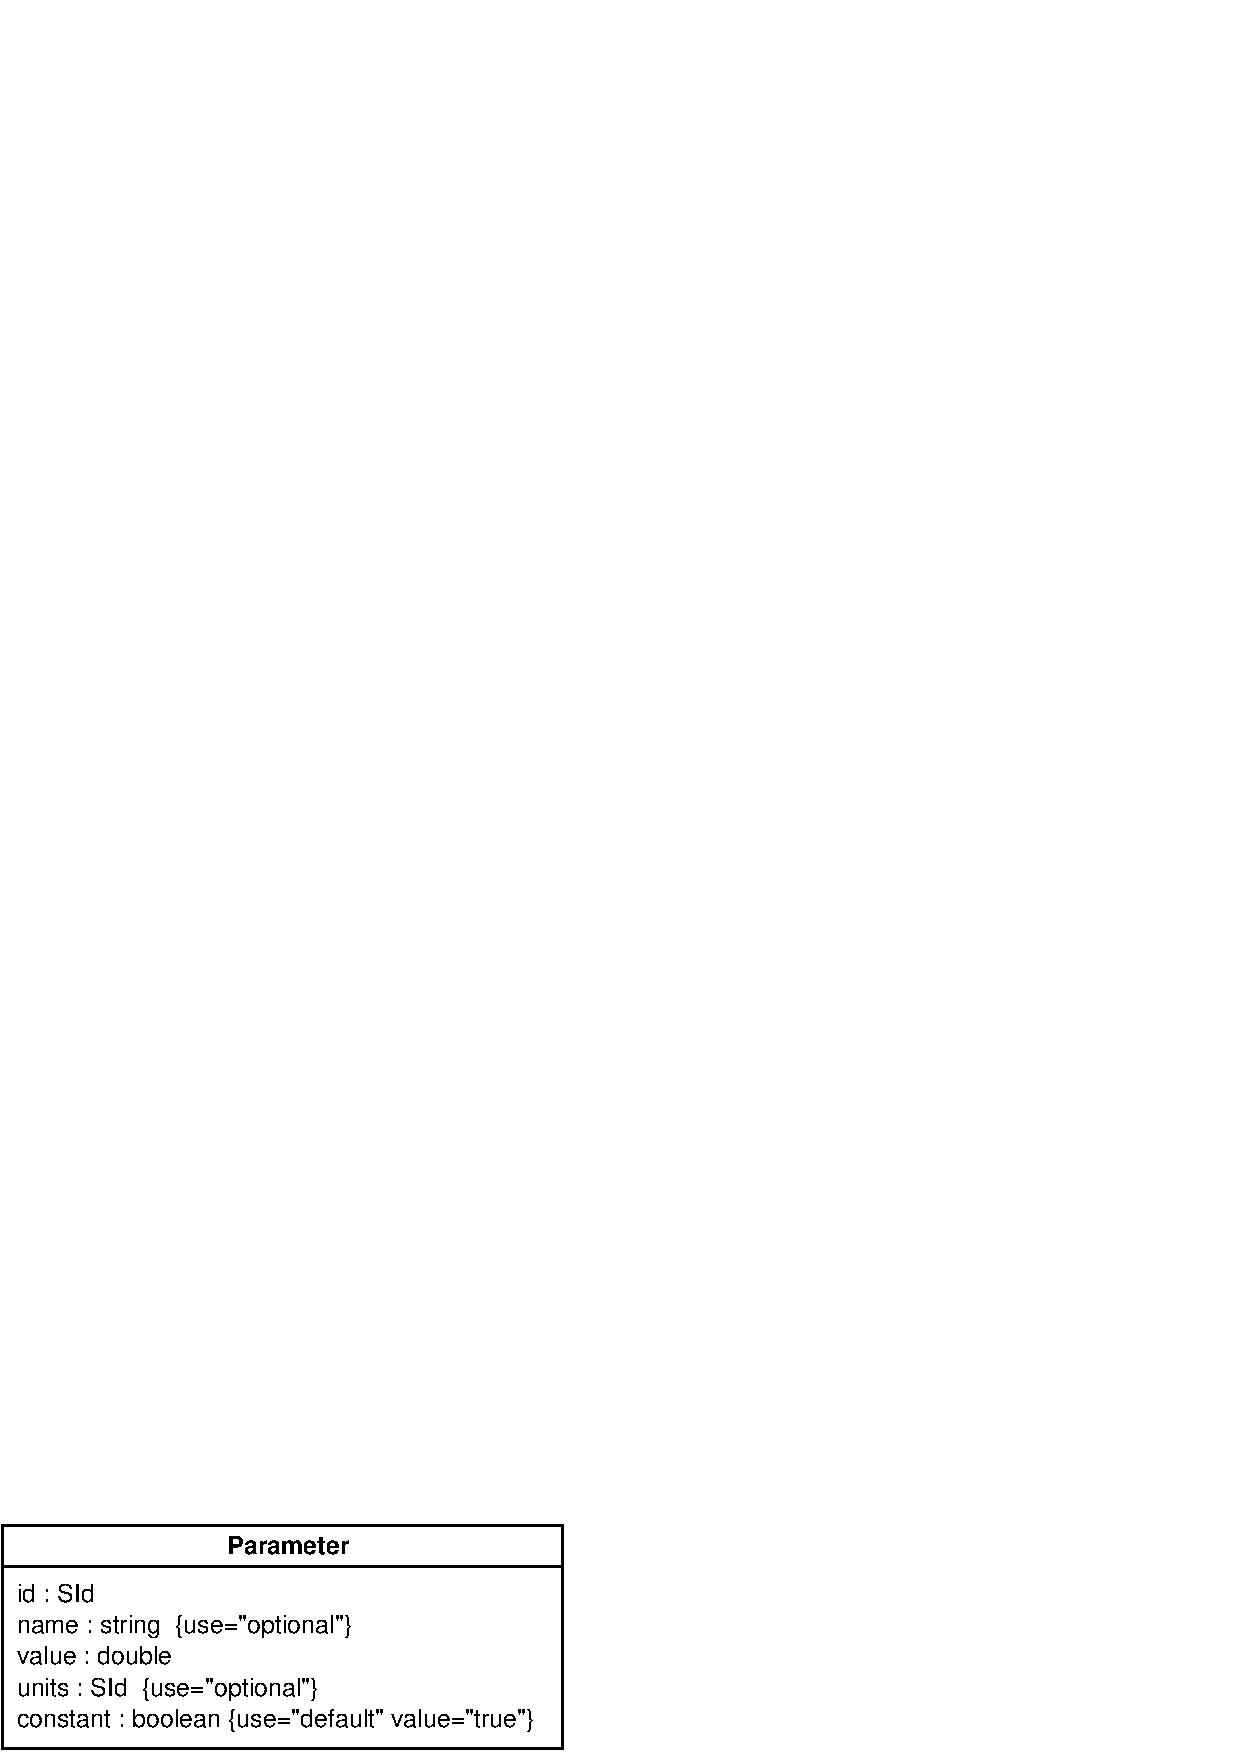
\includegraphics[scale = 0.68]{parameter}
  \caption{The definition of \class{Parameter}.   Fields inherited from
    \class{SBase} are omitted here but are assumed.}
  \label{fig:parameter}
\end{figure}

\subsubsection{The \attrib{id} and \attrib{name} Fields}

\class{Parameter} has one required field, \attrib{id}, of type \class{SId},
to give the parameter a unique identifier by which other parts of an SBML
model definition can refer to it.  A parameter can also have an optional
\attrib{name} field of type \class{string}.  Identifiers and names should
be used according to the guidelines described in
Section~\ref{sec:idnameattribs}.

\subsubsection{The \attrib{value} Field}

The optional field
\attrib{value} determines the value (of type \class{double}) assigned to
the identifer.  A missing \attrib{value} implies that the \attrib{value} is
either unknown, determined by an assignment rule, not required for analysis or
available from an external data source.  If the parameter is not constant then
the \attrib{value} field contains the initial value.

\subsubsection{The \attrib{units} Field}
\label{sec:parameter-units}

The units associated with the value of the parameter are specified by the
field \attrib{units}.  These units are used when the parameter identifier
appears in MathML expressions and in \class{AssignmentRule} structures
setting the value of the parameter.  A \class{RateRule} structure which may
determine the value of the parameter has units \quantity{parameter
  units}/\quantity{time}, where \quantity{parameter units} are the units
assigned to the parameter and \quantity{time} is the built-in \unit{time}
units.  The value assigned to the parameter's \attrib{units} attribute must
be chosen from one of the following possibilities: one of the base unit
names from Table~\vref{tab:unitkind}; one of the built-in unit names
appearing in first column of Table~\vref{tab:builtin}); or the name of a
new unit defined in the list of unit definitions in the enclosing
\class{Model} structure.  There are no constraints on which units can be
chosen from these sets.  There are no default units for parameters.

\subsubsection{The \attrib{constant} Field}

The \class{Parameter} structure has an optional boolean field named
\attrib{constant} which indicates whether the parameter's value can vary
during a simulation.  The field's default value is ``\attribvalue{true}'';
a value of ``\attribvalue{false}'' indicates that the parameter's value can
be changed by rules (see Section~\ref{sec:rules}) and that the
\attrib{value} is actually intended to be the initial value of the
parameter.

\subsubsection{Local and Global Parameters}

Parameters can be defined in two places in SBML: in lists of parameters
defined at the top level in a \class{Model}-type structure, and within
individual reaction definitions (as described in
Section~\ref{sec:reactions}).  Parameters defined at the top level are
\emph{global} to the whole model; parameters that are defined within a
reaction are local to the particular reaction and (within that reaction)
\emph{override} any global parameters having the same names.  (See
Section~\ref{sec:namespaces} for further details.)  Parameters local to a
reaction cannot be changed by rules and therefore are implicitly always
constant; thus, parameter definitions within \class{Reaction} structures
should not have a \attrib{constant} attribute value.

\subsubsection{Example}

The following is an example of parameters defined at the \class{Model} level:
\begin{example}
<model>
    ...
    <listOfParameters>
        <parameter id="tau1" value="2.3" units="second"/>
        <parameter id="Km1" value="10.7" units="moleperliter"/>
    </listOfParameters>
    ...
</model>

\end{example}

%-----------------------------------------------------------------------------
\subsection{Rules}
\label{sec:rules}
%-----------------------------------------------------------------------------

In SBML, \emph{rules} provide a way to create constraints on variables for
cases in which the constraints cannot be expressed using reactions
(Section~\ref{sec:reactions}) nor the assignment of an initial value to a
component in a model.  There are two orthogonal dimensions by which rules
can be described.  First, there are three different possible functional
forms, corresponding to the following three general cases (where $x$ is a
variable, $f$ is some arbitrary function, $V$ is a vector of variables that
may not include $x$, and $W$ is a vector of variables that may include $x$):
\begin{center}
\begin{tabular}{rll}
\emph{Algebraic}    & left-hand side is zero:             & $0 = f(W)$\\
\emph{Assignment}  & left-hand side is a scalar:         & $x = f(V)$\\
\emph{Rate}         & left-hand side is a rate-of-change: & $dx/dt = f(W)$
\end{tabular}
\end{center}

The second dimension concerns the role of variable $x$ in the equations
above: $x$ can be the identifier of a compartment (to set its size), a
species (to set its concentration), or a parameter (to set its value).

In their general form given above, there is little to distinguish between
\emph{assignment} and \emph{algebraic} rules.  They are treated as separate
cases for the following reasons:
\begin{itemize}
  
\item \emph{Assignment} rules can simply be evaluated to calculate intermediate
  values for use in numerical methods;
  
\item Some simulators do not contain numerical solvers capable of solving
  unconstrained \emph{algebraic} equations;
  
\item Those simulators that \emph{can} solve these \emph{algebraic}
  equations make a distinction between the different categories listed
  above; and
  
\item Some specialized numerical analyses of models may only be applicable to
  models that do not contain \emph{algebraic} rules.
\end{itemize}

The approach taken to covering these cases in SBML is to define an abstract
\class{Rule} structure that contains only one field, \attrib{math}, to hold
the right-hand side expression, then to derive subtypes of \class{Rule}
that add fields to distinguish the cases of algebraic, assignment and rate
rules.  Figure~\vref{fig:rules} gives the definitions of \class{Rule} and
the subtypes derived from it.  The figure shows there are three subtypes,
\class{AlgebraicRule}, \class{AssignmentRule} and \class{RateRule} defined
directly from \class{Rule}.  These correspond to the cases
\emph{Algebraic}, \emph{Assignment} and \emph{Rate} described above
respectively.

\begin{figure}[htb]
  \centering
  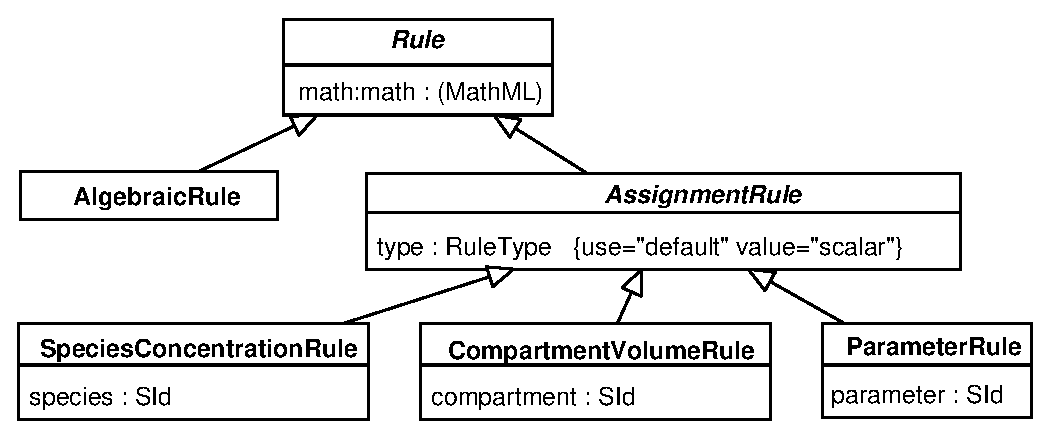
\includegraphics[scale = 0.68]{rule}
  \caption{The definition of \class{Rule} and derived types.}
  \label{fig:rules}
\end{figure}

\subsubsection{\class{AlgebraicRule}}
\label{sec:algebraicrule}

The rule type \class{AlgebraicRule} is used to express equations that are
neither assignments of model variables nor rates of change.
\class{AlgebraicRule} does not add any fields to the basic \class{Rule};
its role is simply to distinguish this case from the other cases.  An
 example of the use of \class{AlgebraicRule} structures is given in
Section~\ref{sec:algeraiceg}.

\subsubsection{\class{AssignmentRule}}
\label{sec:assignmentrule}

The rule type \class{AssignmentRule} is used to express equations that set
the values of variables.  The left-hand side (the \attrib{variable} field
of an assignment rule) of a rule can refer to the identifier of a species,
compartment, or parameter.  Two or
more \class{RateRule} or \class{AssignmentRule} structures cannot have the
same left-hand side or \attrib{variable} attribute value in an SBML model definition.
In all cases, as would be expected, the units of the formula representing the
right hand side, the \attrib{math} field, are identical to the units associated with the
left hand side, the \attrib{variable} field, when that variable appears in other
formulae.

The effects of an \class{AssignmentRule} structure are in general terms
the same, but differ in the precise details depending on which variable is being set:

\begin{itemize}
  
\item \emph{In the case of a species}, an \class{AssignmentRule} sets the
  referenced species' concentration to the value determined by the formula
  in \attrib{math}.  The units of the formula are the \emph{units of the species} as
  defined in Section~\ref{sec:species-units}. (These units can be thought of
  as concentration units if a broad definition of concentration is adopted.)

  \emph{Restrictions}: In a given SBML model, there cannot be both a
  \class{AssignmentRule} \attrib{variable} attribute and a \class{SpeciesReference}
  \attrib{species} attribute that have the same
  value. (See Section~\ref{sec:reactions} for the definition of
  \class{SpeciesReference}.)  This means that an assignment rule cannot be
  defined for a species that is created or destroyed in a reaction.  The
  only exception is when the given species is a boundary condition; i.e.,
  on the \class{Species} structure that defines the species the
  \attrib{boundaryCondition} field is set to ``\attribvalue{true}''.  
  
\item \emph{In the case of a compartment}, an \class{AssignmentRule} sets
  the referenced compartment's size to the size determined by the formula
  in \attrib{math}.  The overall units of the formula are the units
  specified for the size of the compartment identified by the value of the
  \class{AssignmentRule}'s \attrib{variable} field.  (See
  Section~\ref{sec:compartment-units} for an explanation of how the units of the
  compartment's size are determined.)
  
\item \emph{In the case of a parameter}, an \class{AssignmentRule} sets the
  referenced parameter's value to that determined by the formula in
  \attrib{math}.  The overall units of the formula are the units
  defined for the parameter identified by the value of the
  \class{AssignmentRule}'s \attrib{variable} field.  (See
  Section~\ref{sec:parameter-units} for an explanation of how the units of the
  parameter are determined.)
  

\end{itemize}

\subsubsection{\class{RateRule}}
\label{sec:raterule}

The rule type \class{RateRule} is used to express equations that determine
the rates of change of variables.  The left-hand side (the
\attrib{variable} of a rate rule) can refer to the identifier of a species,
compartment, or parameter.  Two or
more \class{RateRule} or \class{AssignmentRule} structures cannot have the
same left-hand side or \attrib{variable} attribute value in an SBML model definition.
In all cases, as would be expected, the units of the formula representing the
right hand side, in the \attrib{math} field, are of the form \quantity{x}/\quantity{time} where
\quantity{x} are the same units as associated with the symbol 
in the \attrib{variable} field, when that variable appears in other
formulae.  \quantity{time} is a built-in unit (see Section~\ref{sec:unitdefinitions}).
The effects of a \class{RateRule} are in general terms the same, but
differ in the precise details depending on which variable is being set:

\begin{itemize}
  
\item \emph{In the case of a species}, a \class{RateRule} sets the rate of
  change of the species's concentration to the value determined by the
  formula in \attrib{math}.  The overall units of the formula must be
  \quantity{concentration}/\quantity{time}, where the \quantity{time} units
  are the built-in units of time described in
  Section~\ref{sec:unitdefinitions} and the \quantity{concentration} units
  are the \emph{units of the species} as
  defined in Section~\ref{sec:species-units}. (A broad definition of concentration
  is used here.)
  
  \emph{Restrictions}: In a given SBML model, there cannot be both a
  \class{RateRule} \attrib{variable} attribute and a \class{SpeciesReference}
  \attrib{species} attribute that have the same
  value. (See Section~\ref{sec:reactions} for the definition of
  \class{SpeciesReference}.)  This means that an assignment rule cannot be
  defined for a species that is created or destroyed in a reaction.  The
  only exception is when the given species is a boundary condition; i.e.,
  on the \class{Species} structure that defines the species the
  \attrib{boundaryCondition} field is set to ``\attribvalue{true}''.  
  
\item \emph{In the case of a compartment}, a \class{RateRule} sets the rate
  of change of the compartment's size to the value determined by the
  formula in \attrib{math}.  The overall units of the formula are
  \quantity{size}/\quantity{time}, where the \quantity{time} units are the
  built-in units of time described in Section~\ref{sec:unitdefinitions} and
  the \quantity{size} units are the units of size on the compartment
  identified by the value of the \class{RateRule}'s \attrib{variable}
  field.  (See Section~\ref{sec:compartment-units} for an explanation of how the
  units of the compartment's size are determined.)

\item \emph{In the case of a parameter}, a \class{RateRule} sets the rate
  of change of the parameter's value to that determined by the formula in
  \attrib{math}.  The overall units of the formula are of the form
  \quantity{x}/\quantity{time} where \quantity{x} is the units
  defined for the parameter identified by the value of the
  \class{AssignmentRule}'s \attrib{variable} field and the \quantity{time}
  units are the built-in units of time described in Section~\ref{sec:unitdefinitions}.  (See
  Section~\ref{sec:parameter-units} for an explanation of how the units of the
  parameter are determined.)
  
\end{itemize}

\subsubsection{Constraints on rules}
\label{sec:ruleconstraints}

SBML specifically does not stipulate the form of the algorithms that can be
applied to rules and reactions.  For example, SBML does not specify when or
how often rules should be evaluated.  The constraints described by rules
and kinetic rate laws are meant to apply collectively to the set of
variable values for a specific instant in time.

The ordering of assignment rules is significant: they are always evaluated
in the order given in SBML.

No more than one assignment or rate rule can be defined for a given
identifier.  No assignment or rate rule can be defined for an identifier
whose corresponding structure has the field \attrib{constant} set to
\attribvalue{true}.

An assignment rule for a given identifier overrides the initial value
assigned to that identifier; i.e., the initial value should be ignored.
This does not mean that any structure declaring an identifier can be
omitted if there is an assignment rule for that identifier.  For example,
there must be a \texttt{Parameter} structure for a given parameter if there
is a rule for that parameter.

The \attrib{math} field of an assignment rule structure can contain any
identifier in a MathML \class{ci} element except for the following: (a)
identifiers for which there exists a subsequent assignment rule, and (b)
the identifier for which the rule is defined.  These constraints are
designed to eliminate algebraic loops among the scalar rules; eliminating
algebraic loops ensures that assignment rules can be evaluated any number
of times without the result of those evaluations changing.  As an example,
consider the following equations, in the order shown:
\begin{equation*}
  \begin{array}{lll}
    x = x + 1, & y = z + 200, & z = y + 100
  \end{array}
\end{equation*}
If this set of equations were interpreted as a set of assignment rules, it
would be invalid because the rule for $x$ refers to $x$ and the rule for
$y$ refers to $z$ before $z$ is defined.


\subsubsection{Example of Rule Use}
\label{sec:eg-rule-use}

This section contains an example set of rules.  Consider the following
set of equations:
\begin{equation*}
  \begin{array}{lll}
    k = \D\frac{k_3}{k_2}, & s_2 = \D\frac{k \, x}{1 + k_2}, & A = 0.10 \, x
  \end{array}
\end{equation*}
This can be encoded by the following scalar rule set (where the definitions
of \texttt{x}, \texttt{s}, \texttt{k}, \texttt{k2}, \texttt{k3} and \texttt{A} are
assumed to be located elsewhere in the model and not shown in this
abbreviated example):
\begin{example}
<model>
    ...
    <listOfRules>
        <assignmentRule variable="k">
            <notes>
                <xhtml:p>
                    k = k3/k2
                </xhtml:p>
            </notes>
            <math xmlns="http://www.w3.org/1998/Math/MathML">
                <apply>
                    <divide/>
                    <ci> k3 </ci>
                    <ci> k2 </ci>
                </apply>
            </math>
        </assignmentRule>
        <assignmentRule variable="s2">
            <notes>
                <xhtml:p>
                    s2 = (k * x)/(1 + k2)
                </xhtml:p>
            </notes>
            <math xmlns="http://www.w3.org/1998/Math/MathML">
                <apply>
                    <divide/>
                    <apply>
                        <times/>
                        <ci> k </ci>
                        <ci> x </ci>
                    </apply>
                    <apply>
                        <plus/>
                        <cn> 1 </cn>
                        <ci> k2 </ci>
                    </apply>
                </apply>
            </math>
        </assignmentRule>
        <assignmentRule variable="A">
            <notes>
                <xhtml:p>
                    A = 0.10 * x
                </xhtml:p>
            </notes>
            <math xmlns="http://www.w3.org/1998/Math/MathML">
                <apply>
                    <times/>
                    <cn> 0.10 </cn>
                    <ci> x </ci>
                </apply>
            </math>
        </assignmentRule>
    </listOfRules>
    ...
</model>

\end{example}


%\subsubsection{Guidelines for Evaluating Rules}
%
%This section describes how rules including those implied by
%\class{Reaction} structures (see Section~\ref{sec:reactions})
%should be evaluated.  For the purpose of interpreting models
%mathematically (and for this description), \class{Reaction}
%structures collectively imply a \class{SpeciesConcentrationRule}
%structure, of type \class{rate}, for each species referenced in a
%\class{SpeciesReference} structure excluding those species which
%are defined with the \attrib{boundaryCondition} attribute equal to
%\texttt{true}.
%
%To determine the initial values of variables is a 2 set process:
%
%\begin{itemize}
%
%\item variables should be set according to the initial values
%given by \class{Species}, \class{Compartment} and
%\class{Parameter} structures then
%
%\item the \class{scalar} rules should be evaluated
%
%\end{itemize}
%
%To determine the rates of change of variables given a set of
%current variable values is again a two set process:
%
%\begin{itemize}
%
%\item the \class{scalar} rules should be evaluated then
%
%\item the \class{rate} rules should be evaluated
%
%\end{itemize}
%
%The \class{scalar} rules should be evaluated to determine the
%complete set of variable values given an incomplete set of
%variable values determined by \class{rate} and
%\class{AlgebraicRule} structures.
%

%-----------------------------------------------------------------------------
\subsection{Reactions}
\label{sec:reactions}
%-----------------------------------------------------------------------------

A \emph{reaction} represents any transformation, transport or binding
process, typically a chemical reaction, that can change the
amount of one or more species.  In SBML, a reaction is defined primarily in
terms of the participating reactants and products (and their corresponding
stoichiometries), along with optional modifier species, an optional kinetic
law describing the rate at which the reaction takes place, and optional
parameters entering into the kinetic law.  These various parts of a
reaction are recorded in the SBML \class{Reaction} type defined in
Figure~\vref{fig:reaction}.

\begin{figure}[htb]
  \vspace*{20pt}
  \centering
  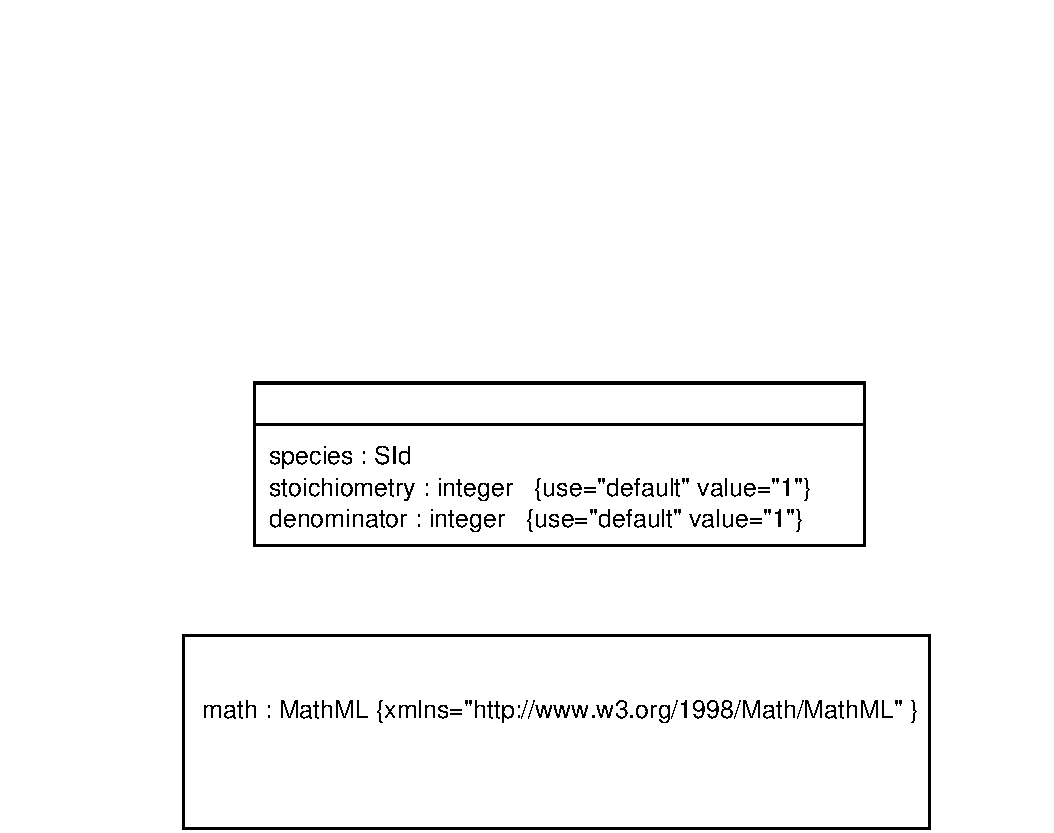
\includegraphics[scale=0.67]{reaction}
  \caption{The definitions of \class{Reaction}, \class{KineticLaw},
    \class{SpeciesReference} and \class{ModiferSpeciesReference}.}
  \label{fig:reaction}
\end{figure}

\subsubsection{The \attrib{id} and \attrib{name} Fields} 

As with most other main structures in SBML, the \class{Reaction} data
structure includes a required \attrib{id} and an optional
\class{name}.  These must be used according to the guidelines described in
Section~\ref{sec:idnameattribs}.

\subsubsection{The \attrib{reactant}, \attrib{product} and \attrib{modifier} Fields}

The reactant species, product species and
modifier species in a reaction are described using the fields
\attrib{reactant}, \attrib{product} and \attrib{modifiers}, respectively.
These fields are optional lists of \class{SpeciesReference} and
\class{ModifierSpeciesReference} structures, as shown in
Figure~\vref{fig:reaction}.  They are described in more detail in
Sections~\ref{subsec:speciesreference} and~\ref{subsec:modifierreference}
below.  The abstract type \class{SimpleSpeciesReference} is shown
simply to demonstrate the common attribute, \attrib{species},
of the \class{SpeciesReference} and
\class{ModifierSpeciesReference} structures.  In future levels of SBML
it is anticipated that \class{SimpleSpeciesReference} will have additional
attributes.

\subsubsection{The \attrib{reversible} Field}

The \attrib{reversible} optional boolean field indicates
whether the reaction is reversible.  The field is optional, and if left
unspecified in a model, it defaults to a value of ``\attribvalue{true}''.
Although the reversibility of a reaction is determined by its rate law, the
need to allow rate expressions in SBML to be optional leads to the need for
a flag indicating reversibility.  Information about reversibility in the
absence of a \attrib{KineticLaw} in a \class{Reaction} is useful in certain
kinds of structural analyses such as elementary mode analysis.  It is true
that the presence of this information in two places (i.e., the rate
expression and the flag \attrib{reversible}) leaves open the possibility of
a model containing contradictory information, but the creation of such a
model would indicate an error on the part of the software generating it.
Software developers must take care to ensure against logical contradictions
in the definitions of reactions.

\subsubsection{The \attrib{fast} Field}

The optional boolean field \attrib{fast} is another boolean attribute in the
\class{Reaction} data structure; a value of ``\attribvalue{true}''
signifies that the given reaction is a ``fast'' one compared to others in
the system being modeled.  This may be relevant when computing equilibrium
concentrations of rapidly equilibrating reactions.  Simulation/analysis
packages may chose to use this information to reduce the number of ODEs
required and thereby optimize such computations.  (A simulator/analysis package
that has no facilities for dealing with fast reactions can ignore this
attribute. In theory, if the choice of which reactions are fast is
correctly made, then a simulation performed with them should give the same
results as a simulation performed without fast reactions.  However,
currently there appears to be no single unambiguous method for designating
which reactions should be considered fast, and some users may designate a
reaction as fast when in fact it is not.)  The \attrib{fast} attribute
does not have a default value: a missing value indicates that the
modeller doesn't know or doesn't wish to specify the rate of the
reaction relative to other reactions in the model.

\subsubsection{\class{SpeciesReference}}
\label{subsec:speciesreference}

Every species that enters into a given reaction must appear in that
reaction's lists of reactants, products or modifiers.  In an SBML model,
all species that participate in any reaction are listed in the
\attrib{listOfSpecies} field of the top-level \class{Model} data structure
(see Section~\ref{sec:model}).  Lists of products, reactants and modifiers
in \class{Reaction} type structures do not introduce new species, but
rather, they refer back to those listed in the model's
\attrib{listOfSpecies}.  For reactants and products, the connection is
made using the \class{SpeciesReference} type data structure defined
in Figure~\vref{fig:reaction}.

In \class{SpeciesReference}, the field \attrib{species} of type \class{SId}
must refer to the name of an existing species defined in the enclosing
\class{Model}-type structure.  The stoichiometry for the product or
reactant can be specified using either the \attrib{stoichiometry} or
\attrib{stoichiometryMath} fields of the
\class{SpeciesReference} structure. The \attrib{stoichiometry} field is of
type double and defaults to 1.  It is recommended for maximal interoperability that
this field is used in preference to the \attrib{stoichiometryMath} field and
should contain an integer value (see the following
example).  The \attrib{stoichiometryMath} field is implemented
as an element containing a MathML math expression in
dimensionless units.  Only one of the \attrib{stoichiometry} and
\attrib{stoichiometryMath} fields should be used on a given \class{SpeciesReference}
structure.

The following is a simple example of a species reference for species
``X0'', with stoichiometry 2, in a list of reactants within a reaction
named ``J1'':
\begin{example}
<model>
    ...
    <listOfReactions>
        <reaction id="J1">
            <listOfReactants>
                <speciesReference species="X0" stoichiometry="2">
            </listOfReactants>
            ...
        </reaction>
        ...
    </listOfReactions>
    ...
</model>
\end{example}

The following is a more complex example of a species reference for species
``X0'', with a stoichiometry expression consisting of the parameter \texttt{x}:
\begin{example}
<model>
    ...
    <listOfReactions>
        <reaction id="J1">
            <listOfReactants>
                <speciesReference species="X0">
                    <stoichiometryMath>
                        <math xmlns="http://www.w3.org/1998/Math/MathML">
                            <ci>x</ci>
                        </math>
                    </stoichiometryMath>
                </speciesReference>
            </listOfReactants>
            ...
        </reaction>
        ...
    </listOfReactions>
    ...
</model>
\end{example}

A reaction can contain an empty list of reactants or an empty list of
products but must have at least one reactant or product.  Also note that
whether a given species is allowed to appear as a reactant or product is
dictated by certain flags on the structure describing the species in the
\class{Model}; see Table~\vref{tab:specieattrib} for more information.

A species can occur more than once in the lists of reactants and products of a given
reaction.  Such a \class{Reaction} structure represents the combined effect of all
the \class{SpeciesReference} structures that are contained in it.  The effective
stoichiometry for a species in a reaction is the sum of
the stoichiometry values given on the \class{SpeciesReference} structures in the list
of products minus the sum of stoichiometry values given on the
\class{SpeciesReference} structures in the list of reactants.  
A positive value indicates that the species is effectively a product and a negative
value indicates that the species is effectively a reactant.  SBML places no
restrictions on the effective stoichiometry of a species in a reaction, for example,
it can be zero.  In the following two SBML fragment, the 2 reactions have the same
effective stoichiometry for all their species.

\begin{example}
<reaction id="x">
    <listOfReactants>
        <speciesReference species="a"/>
        <speciesReference species="a"/>
        <speciesReference species="b"/>
    </listOfReactants>
    <listOfProducts>
        <speciesReference species="c"/>
        <speciesReference species="b"/>
    </listProducts>
</reaction>
<reaction id="y">
    <listOfReactants>
        <speciesReference species="a" stoichiometry="2"/>
    </listOfReactants>
    <listOfProducts>
        <speciesReference species="c"/>
    </listProducts>
</reaction>
\end{example}

\subsubsection{\class{ModifierSpeciesReference}}
\label{subsec:modifierreference}

In some cases, a species may act as a catalyst or inhibitor of a
reaction and would not appear in the list of reactants or products
because it is neither created nor destroyed in that reaction. In these
cases, the species is known as a modifier. (That same species may still be
a reactant or product of another reaction.)

The \class{Reaction} structure provides a way to express which species act
as modifiers in a given reaction.  This is the purpose of the
\attrib{modifier} field in \class{Reaction}; this field is a list of
\class{ModifierSpeciesReference} structures defined in
Figure~\vref{fig:reaction}.  The \class{ModifierSpeciesReference} structure
has only one field, \attrib{species}, of type \class{SId}; its value must
be the identifier of a species defined in the enclosing \class{Model}.

\subsubsection{\class{KineticLaw}}
\label{subsec:kinetic-law}

A \class{kineticLaw} structure, enclosed in a \class{Reaction} structure,
 describes the rate at which the reaction
takes place.  The inclusion of a \class{KineticLaw} structure in an
instance of a \class{Reaction} component is optional; however, in general
there is no useful default that can be substituted in place of a missing
rate law definition in a reaction.
As shown in Figure~\vref{fig:reaction}, the \class{KineticLaw} structure has a
field called \attrib{math}; this is a MathML expression that defines the
rate of the reaction.  

It is important to make clear at the outset that a ``kinetic law'' in SBML
is \emph{not} equivalent to a traditional rate law.  The reason is that
SBML must support multi-compartment models, and the units used in textbook
rate laws as well as some conventional single-compartment modeling packages
are problematic when used for defining reactions between multiple
compartments.  Rate expressions in SBML are expressed in terms of
\quantity{substance}/\quantity{time}, rather than the more typical
\quantity{concentration}/\quantity{time}.  Converting between these two
conventions is a simple matter of dividing the
\quantity{substance}/\quantity{time} expression by the size of the
compartment where a given species is located.  To put this in slightly more
precise terms, suppose that there are two species $S$ and $P$ in a reaction
$S \rightarrow P$, where $S$ is located in a compartment $A$ having
volume $V_A$, $P$ is located in a compartment $B$ having volume $V_B$, and
the kinetic law expression gives the rate of the reaction as being $R$.
Then the rate of change in the concentration of $S$ is given by $d[S]_A/dt
= -R/V_A$ and the rate of change in the concentration of $P$ is $d[P]_B/dt
= R/V_B$.  The translation of a complete multi-compartmental model into
ODEs is given in Section~\ref{sec:odeeg}.

The expression in \attrib{math} may refer to
species identifiers; in that case, as discussed in
Section~\ref{sec:ci-token}, the units of each species reference are
those of \quantity{concentration}.  The only species identifiers that can
be used in \attrib{math} are those listed in the \attrib{reactant},
\attrib{product} and \attrib{modifier} fields of the \class{Reaction}
structure.

As was previously stated the overall rate expression in the \attrib{math} field must
have the units of \quantity{substance/time}.  The optional fields
\attrib{substanceUnits} and \attrib{timeUnits} determine the units of
substance and time for the reaction respectively.
The values of these fields must be
chosen from one of the following possibilities: one of the base
unit names from Table~\vref{tab:unitkind}; one of the built-in unit names
appearing in first column of Table~\vref{tab:builtin}); or the name of a new
unit defined in the list of unit definitions in the enclosing \class{Model}
structure.  In the case of \attrib{substanceUnits}, the value chosen must be a
scaled and/or multiplied variant of \unit{moles} or \unit{item}.
In the case of \attrib{timeUnits}, the value chosen must be a scaled and/or multiplied
variant of \unit{seconds}.
If these fields are not set in a
given \class{KineticLaw} instance, the units are taken from the defaults
defined by the built-in ``\unit{substance}'' and ``\unit{time}'' of
Table~\vref{tab:builtin}.  

An instance of a \class{KineticLaw} type structure can contain zero or more
\class{parameter} structures (Section~\ref{sec:parameters}) that define
symbols that can be used in the \attrib{math} field.  As discussed in
Section~\ref{sec:namespaces}, reactions introduce local namespaces for
parameter identifiers.  Within a \class{KineticLaw} structure inside a
reaction definition, a local parameter whose identifier is identical to a
global parameter defined in the enclosing \class{Model}-type structure
takes precedence over that global parameter.

The following is an example of a \class{Reaction} structure that defines a
reaction named $J_1$, in which $X_0 \rightarrow S_1$ at a rate given by
$k X_0 S_2$, where $S_2$ is a catalyst and $k$ is a parameter.  It
demonstrates the use of species references and the \class{KineticLaw}
structure.  The units on the species here are the defaults of
\quantity{substance}/\quantity{volume} (see Section~\ref{sec:species}), and
so the units of the parameter $k$ are set appropriately to make the rate
expression have final units of \quantity{substance/time}.
\begin{example}
<model>
    ...
    <listOfUnitDefinitions>
        <unitDefinition id="vol_per_concent_per_time">
            <listOfUnits>
                <unit kind="litre"  exponent="2"/>
                <unit kind="mole"   exponent="-1"/>
                <unit kind="second" exponent="-1"/>
            </listOfUnits>
        </unitDefinition>
    </listOfUnitDefinitions>
    ...
    <listOfSpecies>
        <species id="S1" compartment="c1" initialConcentration="2.0"/>
        <species id="S2" compartment="c1" initialConcentration="0.0"/>
        <species id="E1" compartment="c1" initialConcentration="1.0"/>
    </listOfSpecies>
        ...
    <listOfReactions>
        <reaction id="J1">
            <listOfReactants>
                <speciesReference species="S1"/>
            </listOfReactants>
            <listOfProducts>
                <speciesReference species="S2"/>
            </listOfProducts>
            <listOfModifiers>
                <modifierSpeciesReference species="E1"/>
            </listOfModifiers>
            <kineticLaw>
                <math xmlns="http://www.w3.org/1998/Math/MathML">
                    <apply>
                        <times/>
                        <ci> k </ci>
                        <ci> S1 </ci>
                        <ci> E1 </ci>
                    </apply>
                </math>
                <listOfParameters>
                    <parameter id="k" value="0.1" units="vol_per_concent_per_time"/>
                </listOfParameters>
            </kineticLaw>
        </reaction>
    </listOfReactions>
    ...
</model>
\end{example}


%-----------------------------------------------------------------------------
\subsection{Events}
\label{sec:events}
%-----------------------------------------------------------------------------

\class{Model} has an optional list of \class{Event} structures that
describe the time and form of explicit instantaneous discontinuous state
changes in the model.  For example, an event may describe that one species
concentration is halved when another species concentration exceeds a given
threshold value.

An \class{Event} structure defines when the event can occur, the variables
that are affected by the event, and how the variables are affected.  The
effect of the event can optionally be delayed after the occurrence of the
condition which invokes it.  The operation of an \class{Event} structure is
divided into two phases (even when the event is not delayed): one when the
event is \emph{fired} and the other when the event is \emph{executed}. The
\class{Event} type is defined in Figure~\vref{fig:event}.  Both
\class{Event} and \class{EventAssignment} are derived from \class{SBase}
(see Section~\ref{sec:sbase}).  An example of a model which uses events is
given below.

\begin{figure}[htb]
  \centering
  
\includegraphics[scale = 0.68]{event}
  \caption{The definitions of \class{Event} and \class{EventAssignment}}
  \label{fig:event}
\end{figure}

\subsubsection{The \attrib{id} and \attrib{name} Fields}
These optional fields are available to enable to support external references 
to event structures.  These fields operate in the manner described in
Section~\ref{sec:idnameattribs} except that the \attrib{id} field is optional.

\subsubsection{The \attrib{trigger} Field}
The \attrib{trigger} field defines when the \class{Event} structure has an
effect on the model.  The \attrib{trigger} field contains a MathML boolean
expression.  The exact instant that the expression evaluates to true is the
time point when the \class{Event} is \emph{fired}.  The event only fires
when the \attrib{trigger} makes the transition from false to true.  The
event will fire at any further time points when the \attrib{trigger} make
this transition.

\subsubsection{The \attrib{delay} Field}
The optional \attrib{delay} field defines the length of time after
the event has \emph{fired} that the event is \emph{executed}. The
\attrib{delay} field is another MathML expression.  This
expression should be evaluated when the rule is \emph{fired}.  The
default value for the \attrib{delay} field is 0.  The value of the
\attrib{delay} field should always be positive.  The units of the \attrib{delay}
field are those given on the \attrib{timeUnits} field.

\subsubsection{The \attrib{timeUnits} Field}
The optional field \attrib{timeUnits} determines the units of time
that apply to the \attrib{delay} field. 
The value of the \attrib{timeUnits} field must be either
``\unit{second}'' from Table~\vref{tab:unitkind}, ``\unit{time}'' from
Table~\vref{tab:builtin},
or a new unit defined by a unit definition in the enclosing model
which must be a variant of ``\unit{second}'' units.
The default value of the \attrib{timeUnits} field is
``\unit{time}''.

\subsubsection{The \attrib{eventAssignment} Field}
The \attrib{eventAssignment} field consists of a non-empty list of
\class{eventAssignment} structures.  This field is implemented as a
\class{listOfEventAssignments} element containing one or more
\class{eventAssignment} elements.  The \class{EventAssignment}
structures represent variable assignments which have effect when
the event is \emph{executed}. The \class{Assignment} structure is
shown in Figure~\ref{fig:event}. The \attrib{variable} field is of
type \class{SId} and contains the identifier of a variable i.e. a
compartment, species or parameter.  The structures referenced by
the \attrib{variable} field must have their \attrib{constant}
fields set to ``\attribvalue{false}''.  The \attrib{math} field
contains a MathML expression which defines the new value of the
variable.  This expression is evaluated when the \class{Event} is
\emph{fired} but the variable only acquires the result or new
value when the \class{Event} is \emph{executed}.  The order of the
\class{EventAssignment} structures is not significant (unlike
assignment rules), the effect of one assignment cannot affect the
result of another assignment.  The identifiers occurring in the
MathML \attrib{ci} fields of the \class{EventAssignment}
structures represent the value of the identifier at the point when
the \class{Event} is \emph{fired}.

In all cases, as would be expected, the units of the formula are identical to the
units associated with the \attrib{variable} field, when that variable appears in
other formulae.
However the precise details, which are identical to those of \class{AssignmentRule}
structures, depend on which variable is being set:

\begin{itemize}
  
\item \emph{In the case of a species}, an \class{EventAssignment} sets the
  referenced species' concentration to the value determined by the formula
  in \attrib{math}.  The units of the formula are the \emph{units of the species} as
  defined in Section~\ref{sec:species-units}. (These units can be thought of
  as concentration units if a broad definition of concentration is adopted.)

\item \emph{In the case of a compartment}, an \class{EventAssignment} sets
  the referenced compartment's size to the size determined by the formula
  in \attrib{math}.  The overall units of the formula are the units
  specified for the size of the compartment identified by the value of the
  \class{EventAssignment}'s \attrib{variable} field.  (See
  Section~\ref{sec:compartment-units} for an explanation of how the units of the
  compartment's size are determined.)
  
\item \emph{In the case of a parameter}, an \class{EventAssignment} sets the
  referenced parameter's value to that determined by the formula in
  \attrib{math}.  The overall units of the formula are the units
  defined for the parameter identified by the value of the
  \class{EventAssignment}'s \attrib{variable} field.  (See
  Section~\ref{sec:parameter-units} for an explanation of how the units of the
  parameter are determined.)
  
\end{itemize}

\subsubsection{Example \class{Event} structure}

A example of an \class{Event} structure follows.  This structure makes the
assignment $k_2 = 0$ at the point when $P_1 \leq t$:

\begin{example}
<event>
    <trigger>
        <math xmlns="http://www.w3.org/1998/Math/MathML">
            <apply>
                <leq/>
                <ci> P1 </ci>
                <ci> t </ci>
            </apply>
        </math>
    </trigger>
    <listOfEventAssignments>
        <eventAssignment variable="k2">
            <math xmlns="http://www.w3.org/1998/Math/MathML">
                <cn> 0 </cn>
            </math>
        </eventAssignment>
    <listOfEventAssignments>
</event>
\end{example}

A complete example model that uses events is given in Section~\ref{sec:eventeg}

\subsubsection{Detailed semantics of events}

The description of events above describes the action of events in isolation from
each other.  This section describes how events interact.  Events whose \attrib{trigger}
expression is true at the start of a simulation do not \emph{fire} at the start of the simulation.
Events \emph{fire} only when the trigger \emph{becomes} true i.e. the trigger expression
transitions from false to true.  It is possible for events to \emph{fire} other events, i.e. an
event assignment can cause an event to \emph{fire}, therefore it is possible for model to be entirely
encoded in \class{Event} structures.

It is entirely possible for two events to be \emph{executed} simultaneously in simulated time.
It is assumed that, although the precise time at which these events are \emph{executed} is not
resolved beyond the given point in simulated time, the order in which the events occur is resolved.
This order can be significant in determining the overall outcome of a given simulation. SBML Level
2 does not define the algorithm for determining this order (the tie-breaking algorithm).  As a
result the results of simulations involving events may vary when simultaneous events occur during
simulation.  It is anticipated that future versions or levels of SBML will define a specific set
of tie-breaking algorithms and a mechanism for models to indicate which algorithm should be 
applied during simulation.

Despite the absence of a specific tie-breaking algorithm SBML event simulation is constrained as
follows. When an event $X$ \emph{fires} another event $Y$ and event $Y$ has zero delay then event
$Y$ is added to the existing set of simultaneous events that are pending \emph{execution}. Events
such as $Y$ do not have a special priority or ordering within the tie-breaking algorithm. Events
$X$ and $Y$ form a cascade of events at the same point in simulation time.  All events in a model
are open to being in a cascade.  The position of an event in the event list doesn't affect whether
it can be in the cascade: $Y$ can be triggered whether it is before or after $X$ in the list of
events.  A cascade of events can be infinite (never terminate).  When this occurs a simulator
should indicate this has occurred i.e. it is incorrect for the simulator to arbitrarily break the
cascade and continue the simulation without at least indicating the infinite cascade occurred.
Given that a variable can change more than once when processing simultaneous events at simulation
time $t$ then the model behavior (output) for that variable at time $t$ is the value of the
variable at the end of processing all the simultaneous events at time $t$.

%=============================================================================
\section{Example Models Expressed in XML Using SBML}
\label{sec:xml-rep}
\label{sec:examples}
%=============================================================================

In this section, we present several examples of complete models
encoded in XML using SBML Level~2.  

%Our approach to translating
%the UML-based structure definitions presented in the previous
%sections is described elsewhere~\citep{hucka:2000b}.
%Appendix~\ref{apdx:schemas} gives the full listing of an XML
%Schema corresponding to SBML Level~2.


%-----------------------------------------------------------------------------
\subsection{A Simple Example Application of SBML}
\label{sec:modeleg}
%-----------------------------------------------------------------------------

Consider the following hypothetical branched system:
\begin{center}
\includegraphics[scale = 0.9]{example-network}
\end{center}
The following is an XML document that encodes the model shown
above:

\begin{example}
<?xml version="1.0" encoding="UTF-8"?>
<sbml xmlns="http://www.sbml.org/sbml/level2" level="2" version="1">
    <model id="Branch">
        <notes>
            <body xmlns="http://www.w3.org/1999/xhtml">
                <p>Simple branch system.</p>
                <p>The reaction looks like this:</p>
                <p>reaction-1:   X0 -> S1; k1*X0;</p>
                <p>reaction-2:   S1 -> X1; k2*S1;</p>
                <p>reaction-3:   S1 -> X2; k3*S1;</p>
            </body>
        </notes>
        <listOfCompartments>
            <compartment id="compartmentOne" size="1"/>
        </listOfCompartments>
        <listOfSpecies>
            <species id="S1" initialConcentration="0" compartment="compartmentOne"
                     boundaryCondition="false"/>
            <species id="X0" initialConcentration="0" compartment="compartmentOne"
                     boundaryCondition="true"/>
            <species id="X1" initialConcentration="0" compartment="compartmentOne"
                     boundaryCondition="true"/>
            <species id="X2" initialConcentration="0" compartment="compartmentOne"
                     boundaryCondition="true"/>
        </listOfSpecies>
        <listOfReactions>
            <reaction id="reaction_1" reversible="false">
                <listOfReactants>
                    <speciesReference species="X0"/>
                </listOfReactants>
                <listOfProducts>
                    <speciesReference species="S1"/>
                </listOfProducts>
                <kineticLaw>
                    <math xmlns="http://www.w3.org/1998/Math/MathML">
                        <apply>
                            <times/>
                            <ci> k1 </ci>
                            <ci> X0 </ci>
                        </apply>
                    </math>
                    <listOfParameters>
                        <parameter id="k1" value="0"/>
                    </listOfParameters>
                </kineticLaw>
            </reaction>
            <reaction id="reaction_2" reversible="false">
                <listOfReactants>
                    <speciesReference species="S1"/>
                </listOfReactants>
                <listOfProducts>
                    <speciesReference species="X1"/>
                </listOfProducts>
                <kineticLaw>
                    <math xmlns="http://www.w3.org/1998/Math/MathML">
                        <apply>
                            <times/>
                            <ci> k2 </ci>
                            <ci> S1 </ci>
                        </apply>
                    </math>
                    <listOfParameters>
                        <parameter id="k2" value="0"/>
                    </listOfParameters>
                </kineticLaw>
            </reaction>
            <reaction id="reaction_3" reversible="false">
                <listOfReactants>
                    <speciesReference species="S1"/>
                </listOfReactants>
                <listOfProducts>
                    <speciesReference species="X2"/>
                </listOfProducts>
                <kineticLaw>
                    <math xmlns="http://www.w3.org/1998/Math/MathML">
                        <apply>
                            <times/>
                            <ci> k3 </ci>
                            <ci> S1 </ci>
                        </apply>
                    </math>
                    <listOfParameters>
                        <parameter id="k3" value="0"/>
                    </listOfParameters>
                </kineticLaw>
            </reaction>
        </listOfReactions>
    </model>
</sbml>
\end{example}

In this example, the model has the identifier ``Branch''.  The model contains one
compartment, four species, and three reactions.  The elements in the
\texttt{<listOfReactants>} and \texttt{<listOfProducts>} in each reaction
refer to the names of elements listed in the \texttt{<listOfSpecies>}.  The
correspondences between the various elements is explicitly stated by the
\texttt{<speciesReference>} elements.

The model also includes a \texttt{<notes>} annotation that summarizes the
model in text form, with formatting encoded in XHTML.  This may be useful for
a software package that is able to read such annotations and, for example,
render them in HTML in a graphical user interface.


%-----------------------------------------------------------------------------
\subsection{Example Involving Units}
\label{apdx:units-eg}
%-----------------------------------------------------------------------------

The following model uses the units features of SBML Level~2.  In
this model, the default value of \unit{substance} is changed in
the list of unit definitions to be mole units with a scale factor
of $-3$, or millimoles.  This sets the default substance units in
the model; components can override this scale locally.  The
\attrib{size} and \attrib{time} built-ins are left to their
defaults, ensuring that size is in liters and time is in
seconds.  The result is that, in this model, kinetic law formulas
define rates in millimoles per second and the species symbols in
them represent concentration values in millimoles per liter.  All
the \class{species} elements set the initial amount of every given
species to 1 millimole.  The parameters \texttt{Vm} and
\texttt{Km} are defined to be in millimoles per liter per second,
and milliMolar, respectively.

\begin{example}
<?xml version="1.0" encoding="UTF-8"?>
<sbml xmlns="http://www.sbml.org/sbml/level2" level="2" version="1"
      xmlns:html="http://www.w3.org/1999/xhtml">
    <model>
        <listOfUnitDefinitions>
            <unitDefinition id="substance">
                <listOfUnits>
                    <unit kind="mole" scale="-3"/>
                </listOfUnits>
            </unitDefinition>
            <unitDefinition id="mmls">
                <listOfUnits>
                    <unit kind="mole" scale="-3"/>
                    <unit kind="litre" exponent="-1"/>
                    <unit kind="second" exponent="-1"/>
                </listOfUnits>
            </unitDefinition>
            <unitDefinition id="mm">
                <listOfUnits>
                    <unit kind="mole" scale="-3"/>
                </listOfUnits>
            </unitDefinition>
        </listOfUnitDefinitions>
        <listOfCompartments>
            <compartment id="cell"/>
        </listOfCompartments>
        <listOfSpecies>
            <species id="x0" compartment="cell" initialConcentration="1"/>
            <species id="x1" compartment="cell" initialConcentration="1"/>
            <species id="s1" compartment="cell" initialConcentration="1"/>
            <species id="s2" compartment="cell" initialConcentration="1"/>
        </listOfSpecies>
        <listOfParameters>
            <parameter id="vm" value="2" units="mmls"/>
            <parameter id="km" value="2" units="mm"/>
        </listOfParameters>
        <listOfReactions>
            <reaction id="v1">
                <listOfReactants>
                    <speciesReference species="x0"/>
                </listOfReactants>
                <listOfProducts>
                    <speciesReference species="s1"/>
                </listOfProducts>
                <kineticLaw>
                    <notes>
                        <html:p>((vm * s1)/(km + s1))*cell</html:p>
                    </notes>
                    <math xmlns="http://www.w3.org/1998/Math/MathML">
                        <apply>
                            <times/>
                            <apply>
                                <divide/>
                                <apply>
                                    <times/>
                                    <ci> vm </ci>
                                    <ci> s1 </ci>
                                </apply>
                                <apply>
                                    <plus/>
                                    <ci> km </ci>
                                    <ci> s1 </ci>
                                </apply>
                            </apply>
                            <ci> cell </ci>
                        </apply>
                    </math>
                </kineticLaw>
            </reaction>
            <reaction id="v2">
                <listOfReactants>
                    <speciesReference species="s1"/>
                </listOfReactants>
                <listOfProducts>
                    <speciesReference species="s2"/>
                </listOfProducts>
                <kineticLaw>
                    <notes>
                        <html:p>((vm * s2)/(km + s2))*cell</html:p>
                    </notes>
                    <math xmlns="http://www.w3.org/1998/Math/MathML">
                        <apply>
                            <times/>
                            <apply>
                                <divide/>
                                <apply>
                                    <times/>
                                    <ci> vm </ci>
                                    <ci> s2 </ci>
                                </apply>
                                <apply>
                                    <plus/>
                                    <ci> km </ci>
                                    <ci> s2 </ci>
                                </apply>
                            </apply>
                            <ci> cell </ci>
                        </apply>
                    </math>
                </kineticLaw>
            </reaction>
            <reaction id="v3">
                <listOfReactants>
                    <speciesReference species="s2"/>
                </listOfReactants>
                <listOfProducts>
                    <speciesReference species="x1"/>
                </listOfProducts>
                <kineticLaw>
                    <notes>
                        <html:p>((vm * x1)/(km + x1))*cell</html:p>
                    </notes>
                    <math xmlns="http://www.w3.org/1998/Math/MathML">
                        <apply>
                            <times/>
                            <apply>
                                <divide/>
                                <apply>
                                    <times/>
                                    <ci> vm </ci>
                                    <ci> x1 </ci>
                                </apply>
                                <apply>
                                    <plus/>
                                    <ci> km </ci>
                                    <ci> x1 </ci>
                                </apply>
                            </apply>
                            <ci> cell </ci>
                        </apply>
                    </math>
                </kineticLaw>
            </reaction>
        </listOfReactions>
    </model>
</sbml>

\end{example}

%-----------------------------------------------------------------------------
\subsection{Example Involving Assignment Rules}
\label{apdx:rules-eg}
%-----------------------------------------------------------------------------
This section contains a model which simulates a system containing
a fast reaction.  This model uses rules to express the mathematics
of the fast reaction explicitly rather than using the implicit
\attrib{fast} field on a reaction element.

The system modeled is
\begin{equation*}
  \begin{array}{@{}ccc@{}}
    X_0 & \underrightarrow{k_1 X_0} & S_1 \\ \\[-4pt]
    S_1 & \underrightarrow{k_f S_1 - k_r S_2} & S_2 \\ \\[-4pt]
    S_2 & \underrightarrow{k_2 S_2} & X_1\\ \\[-4pt]
  \end{array}
\end{equation*}
\begin{equation*}
    k_1 = 0.1, \quad k_2 = 0.15, \quad k_f = K_{eq} 10000, \quad k_r = 10000, \quad K_{eq} = 2.5.
\end{equation*}

This can be approximated with the following system:
\begin{equation*}
  \begin{array}{@{}ccc@{}}
    X_0 & \underrightarrow{k_1 X_0} & T \\ \\[-4pt]
    T & \underrightarrow{k_2 S_2} & X_1\\ \\[-4pt]
  \end{array}
\end{equation*}
\begin{equation*}
  \begin{array}{ll}
    S_1 = \D\frac{T}{1 + K_{eq}}, & S_2 = K_{eq} S_1\\ \\[-4pt]
  \end{array}
\end{equation*}
The following example SBML model encodes the approximate form.

\begin{example}
<?xml version="1.0" encoding="UTF-8"?>
<sbml xmlns="http://www.sbml.org/sbml/level2" level="2" version="1"
      xmlns:math="http://www.w3.org/1998/Math/MathML">
    <model>
        <listOfCompartments>
            <compartment id="cell"/>
        </listOfCompartments>
        <listOfSpecies>
            <species id="X0" compartment="cell" initialConcentration="1"/>
            <species id="X1" compartment="cell" initialConcentration="0"/>
            <species id="T" compartment="cell" initialConcentration="0"/>
            <species id="S1" compartment="cell" initialConcentration="0"/>
            <species id="S2" compartment="cell" initialConcentration="0"/>
        </listOfSpecies>
        <listOfParameters>
            <parameter id="Keq" value="2.5"/>
        </listOfParameters>
        <listOfRules>
            <assignmentRule variable="S1">
                <math xmlns="http://www.w3.org/1998/Math/MathML">
                    <apply>
                        <divide/>
                        <ci> T </ci>
                        <apply>
                            <plus/>
                            <cn> 1 </cn>
                            <ci> Keq </ci>
                        </apply>
                    </apply>
                </math>
            </assignmentRule>
            <assignmentRule variable="S2">
                <math xmlns="http://www.w3.org/1998/Math/MathML">
                    <apply>
                        <times/>
                        <ci> Keq </ci>
                        <ci> S1 </ci>
                    </apply>
                </math>
            </assignmentRule>
        </listOfRules>
        <listOfReactions>
            <reaction id="in">
                <listOfReactants>
                    <speciesReference species="X0"/>
                </listOfReactants>
                <listOfProducts>
                    <speciesReference species="T"/>
                </listOfProducts>
                <kineticLaw>
                    <math xmlns="http://www.w3.org/1998/Math/MathML">
                        <apply>
                            <times/>
                            <ci> k1 </ci>
                            <ci> X0 </ci>
                        </apply>
                    </math>
                    <listOfParameters>
                        <parameter id="k1" value="0.1"/>
                    </listOfParameters>
                </kineticLaw>
            </reaction>
            <reaction id="out">
                <listOfReactants>
                    <speciesReference species="T"/>
                </listOfReactants>
                <listOfProducts>
                    <speciesReference species="X1"/>
                </listOfProducts>
                <kineticLaw>
                    <math xmlns="http://www.w3.org/1998/Math/MathML">
                        <apply>
                            <times/>
                            <ci> k2 </ci>
                            <ci> S2 </ci>
                        </apply>
                    </math>
                    <listOfParameters>
                        <parameter id="k2" value="0.15"/>
                    </listOfParameters>
                </kineticLaw>
            </reaction>
        </listOfReactions>
    </model>
</sbml>
\end{example}

%-----------------------------------------------------------------------------
\subsection{Example Involving Algebraic Rules}
\label{sec:algeraiceg}
%-----------------------------------------------------------------------------

This section contains an example model which contains an
\class{AlgebraicRule} structure.  The model contains a different
formulation of the fast reaction described in
Section~\ref{apdx:rules-eg}.

The system described in Section~\ref{apdx:rules-eg} can be
approximated with the following system:
\begin{equation*}
  \begin{array}{@{}ccc@{}}
    X_0 & \underrightarrow{k_1 X_0} & T \\ \\[-4pt]
    T & \underrightarrow{k_2 S_1} & X_1\\ \\[-4pt]
  \end{array}
\end{equation*}
\begin{equation*}
  \begin{array}{ll}
    S_2 = K_{eq} S_1\\ \\[-4pt]
  \end{array}
\end{equation*}
with the constraint:
\begin{equation*}
  \begin{array}{ll}
    S_1 + S_2 - T = 0\\ \\[-4pt]
  \end{array}
\end{equation*}

The following example SBML model encodes this approximate form.

\begin{example}
<?xml version="1.0" encoding="UTF-8"?>
<sbml xmlns="http://www.sbml.org/sbml/level2" level="2" version="1">
    <model>
        <listOfCompartments>
            <compartment id="cell"/>
        </listOfCompartments>
        <listOfSpecies>
            <species id="X0" compartment="cell" initialConcentration="1"/>
            <species id="X1" compartment="cell" initialConcentration="0"/>
            <species id="T" compartment="cell" initialConcentration="0"/>
            <species id="S1" compartment="cell" initialConcentration="0"/>
            <species id="S2" compartment="cell" initialConcentration="0"/>
        </listOfSpecies>
        <listOfParameters>
            <parameter id="Keq" value="2.5"/>
        </listOfParameters>
        <listOfRules>
            <assignmentRule variable="S2">
                <math xmlns="http://www.w3.org/1998/Math/MathML">
                    <apply>
                        <times/>
                        <ci> Keq </ci>
                        <ci> S1 </ci>
                    </apply>
                </math>
            </assignmentRule>
            <algebraicRule>
                <math xmlns="http://www.w3.org/1998/Math/MathML">
                    <apply>
                        <minus/>
                        <apply>
                            <plus/>
                            <ci> S2 </ci>
                            <ci> S1 </ci>
                        </apply>
                        <ci> T </ci>
                    </apply>
                </math>
            </algebraicRule>
        </listOfRules>
        <listOfReactions>
            <reaction id="in">
                <listOfReactants>
                    <speciesReference species="X0"/>
                </listOfReactants>
                <listOfProducts>
                    <speciesReference species="T"/>
                </listOfProducts>
                <kineticLaw>
                    <math xmlns="http://www.w3.org/1998/Math/MathML">
                        <apply>
                            <times/>
                            <ci> k1 </ci>
                            <ci> X0 </ci>
                        </apply>
                    </math>
                    <listOfParameters>
                        <parameter id="k1" value="0.1"/>
                    </listOfParameters>
                </kineticLaw>
            </reaction>
            <reaction id="out">
                <listOfReactants>
                    <speciesReference species="T"/>
                </listOfReactants>
                <listOfProducts>
                    <speciesReference species="X1"/>
                </listOfProducts>
                <kineticLaw>
                    <math xmlns="http://www.w3.org/1998/Math/MathML">
                        <apply>
                            <times/>
                            <ci> k2 </ci>
                            <ci> S2 </ci>
                        </apply>
                    </math>
                    <listOfParameters>
                        <parameter id="k2" value="0.15"/>
                    </listOfParameters>
                </kineticLaw>
            </reaction>
        </listOfReactions>
    </model>
</sbml>
\end{example}

%-----------------------------------------------------------------------------
\subsection{Example Involving Combinations of
  \attrib{boundaryCondition} and \attrib{constant} Values on \class{Species}
  with \class{RateRule} structures}
\label{sec:constantspecieseg}
%-----------------------------------------------------------------------------

This section contains a model which includes four species each with a
different combination of values of for the \attrib{boundaryCondition} and
\attrib{constant} attributes.

Consider the following hypothetical system:
\begin{equation*}
  \begin{array}{@{}ccc@{}}
    S_1 + S_2 & \underrightarrow{k_1 S_1 S_2 S_3} & S_4 \\ \\[-4pt]
  \end{array}
\end{equation*}
$S_3$ is a catalyst that catalyzes the conversion $S_1$ and $S_2$ into $S_4$.
$S_1$ and $S_2$ are on the boundary of the system ($S_1$ and $S_2$ are reactants
but their values are not determined by a kinetic law). 
The value of $S_1$ is determined over time by the rate rule:
\begin{equation*}
  \begin{array}{l}
    \frac{d S_1}{d t} = k_2 \\ \\[-4pt]
  \end{array}
\end{equation*}
Constant values are:
\begin{equation*}
  \begin{array}{l}
    S_2 = 1 \\ \\
    S_3 = 2 \\ \\
    k_1 = 0.5 \\ \\
    k_2 = 0.1 \\ \\
  \end{array}
\end{equation*}
and initial values are:
\begin{equation*}
  \begin{array}{l}
    S_1 = 0 \\ \\
    S_4 = 0 \\ \\
  \end{array}
\end{equation*}

The value of $S_1$ varies over time so in SBML $S_1$
has a \attrib{constant} attribute with a default value of
``\attribvalue{false}''.  The values of $S_2$ and $S_3$ are fixed so in
SBML they have a \attrib{constant} attribute values of
``\attribvalue{true}''.  $S_3$ only occurs as a modifier so the value of
its \attrib{boundaryCondition} attribute can default to false.  $S_4$ is a
product whose value is determined by a kinetic law and therefore in the
SBML representation has false values, the default values, for both
\attrib{boundaryCondition} and \attrib{constant} attributes.

The following is the XML document that encodes the model shown
above:

\begin{example}
<?xml version="1.0" encoding="UTF-8"?>
<sbml xmlns="http://www.sbml.org/sbml/level2" level="2" version="1">
    <model id="BoundaryCondExampleModel">
        <listOfCompartments>
            <compartment id="compartmentOne" size="1"/>
        </listOfCompartments>
        <listOfSpecies>
            <species id="S1" initialConcentration="0" compartment="compartmentOne"
                boundaryCondition="true" />
            <species id="S2" initialConcentration="1" compartment="compartmentOne"
                boundaryCondition="true" constant="true" />
            <species id="S3" initialConcentration="3" compartment="compartmentOne"
                constant="true"/>
            <species id="S4" initialConcentration="0" compartment="compartmentOne"/>
        </listOfSpecies>
        <listOfParameters>
            <parameter id="k1" value="0.5"/>
            <parameter id="k2" value="0.1"/>
        </listOfParameters>
        <listOfRules>
            <rateRule variable="S1">
                <math xmlns="http://www.w3.org/1998/Math/MathML">
                    <apply>
                        <ci> k2 </ci>
                    </apply>
                </math>
            </rateRule>
        </listOfRules>
        <listOfReactions>
            <reaction id="reaction_1" reversible="false">
                <listOfReactants>
                    <speciesReference species="S1"/>
                    <speciesReference species="S2"/>
                </listOfReactants>
                <listOfProducts>
                    <speciesReference species="S4"/>
                </listOfProducts>
                <listOfModifiers>
                    <modifierSpeciesReference species="S3"/>
                </listOfModifiers>
                <kineticLaw>
                    <math xmlns="http://www.w3.org/1998/Math/MathML">
                        <apply>
                            <times/>
                            <ci> k1 </ci>
                            <ci> S1 </ci>
                            <ci> S2 </ci>
                            <ci> S3 </ci>
                         </apply>
                    </math>
                </kineticLaw>
            </reaction>
        </listOfReactions>
    </model>
</sbml>
\end{example}

%-----------------------------------------------------------------------------
\subsection{Example of translation from a multi-compartmental model to ODEs}
\label{sec:odeeg}
%-----------------------------------------------------------------------------

This section contains a model with 2 compartments, 4 reactions and 2 rate rules.
The model is followed by its complete translation into ODEs.  The model is shown in
figure~\ref{fig:multicomp}.

\begin{figure}[htb]
  \vspace*{20pt}
  \centering
  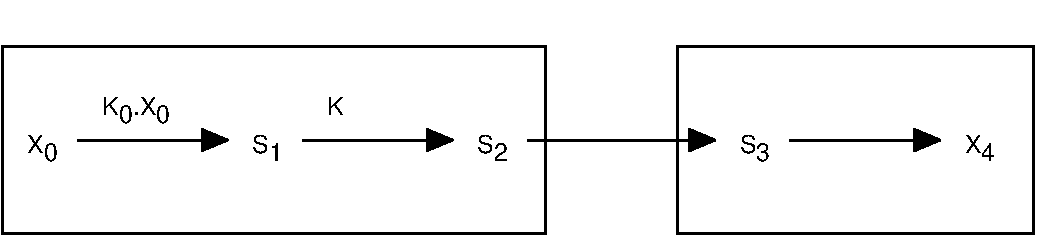
\includegraphics[scale=0.67]{multicomp}
  \caption{A example multi-compartmental model}
  \label{fig:multicomp}
\end{figure}

Reaction equations are in substance per time units.  Species variables are in
concentrations.
Species $X_0$ and $X_4$ are boundary conditions.  The volume of compartment $V_1$
and the concentration of $X_0$ vary according to rules.

The SBML for this model is

\begin{example}
<?xml version="1.0" encoding="UTF-8"?>
<sbml xmlns="http://www.sbml.org/sbml/level2" level="2" version="1">
    <model id="ODEExampleModel">
        <listOfCompartments>
            <compartment id="V0" size="10"/>
            <compartment id="V1" size="1" constant="false"/>
        </listOfCompartments>
        <listOfSpecies>
            <species id="X0" initialConcentration="0" compartment="V0"
                boundaryCondition="true" />
            <species id="S1" initialConcentration="0" compartment="V0"/>
            <species id="S2" initialConcentration="0" compartment="V0"/>
            <species id="S3" initialConcentration="0" compartment="V1"/>
            <species id="X4" initialConcentration="0" compartment="V1"
                boundaryCondition="true" constant="true"/>
        </listOfSpecies>
        <listOfParameters>
            <parameter id="K0" value="0.1"/>
            <parameter id="K1" value="0.5"/>
            <parameter id="K2" value="0.1"/>
            <parameter id="K3" value="0.5"/>
            <parameter id="Kv" value="0.5"/>
            <parameter id="Kin" value="0.1"/>
        </listOfParameters>
        <listOfRules>
            <rateRule variable="X0">
                <math xmlns="http://www.w3.org/1998/Math/MathML">
                    <apply>
                        <ci> Kin </ci>
                    </apply>
                </math>
            </rateRule>
            <rateRule variable="V1">
                <math xmlns="http://www.w3.org/1998/Math/MathML">
                    <apply>
                        <ci> Kv </ci>
                    </apply>
                </math>
            </rateRule>
        </listOfRules>
        <listOfReactions>
            <reaction id="reaction_1" reversible="false">
                <listOfReactants>
                    <speciesReference species="X0"/>
                </listOfReactants>
                <listOfProducts>
                    <speciesReference species="S1"/>
                </listOfProducts>
                <kineticLaw>
                    <math xmlns="http://www.w3.org/1998/Math/MathML">
                        <apply>
                            <times/>
                            <ci> K0 </ci>
                            <ci> X0 </ci>
                         </apply>
                    </math>
                </kineticLaw>
            </reaction>
            <reaction id="reaction_2" reversible="false">
                <listOfReactants>
                    <speciesReference species="S1"/>
                </listOfReactants>
                <listOfProducts>
                    <speciesReference species="S2"/>
                </listOfProducts>
                <kineticLaw>
                    <math xmlns="http://www.w3.org/1998/Math/MathML">
                        <apply>
                            <times/>
                            <ci> K1 </ci>
                            <ci> S1 </ci>
                         </apply>
                    </math>
                </kineticLaw>
            </reaction>
            <reaction id="reaction_3" reversible="false">
                <listOfReactants>
                    <speciesReference species="S2"/>
                </listOfReactants>
                <listOfProducts>
                    <speciesReference species="S3"/>
                </listOfProducts>
                <kineticLaw>
                    <math xmlns="http://www.w3.org/1998/Math/MathML">
                        <apply>
                            <times/>
                            <ci> K2 </ci>
                            <ci> S2 </ci>
                         </apply>
                    </math>
                </kineticLaw>
            </reaction>
            <reaction id="reaction_4" reversible="false">
                <listOfReactants>
                    <speciesReference species="S3"/>
                </listOfReactants>
                <listOfProducts>
                    <speciesReference species="X4"/>
                </listOfProducts>
                <kineticLaw>
                    <math xmlns="http://www.w3.org/1998/Math/MathML">
                        <apply>
                            <times/>
                            <ci> K3 </ci>
                            <ci> S3 </ci>
                         </apply>
                    </math>
                </kineticLaw>
            </reaction>
        </listOfReactions>
    </model>
</sbml>
\end{example}

The ODE translation of this model is as follows assuming all species variables
contain the species concentration:

Parameters and Constants:

\begin{equation*}
  \begin{array}{l}
    X_4 = 0 \\ \\[-4pt]
    V_0 = 10 \\ \\[-4pt]
    K_0 = 0.1\\ \\[-4pt]
    K_1 = 0.5\\ \\[-4pt]
    K_2 = 0.1\\ \\[-4pt]
    K_3 = 0.5\\ \\[-4pt]
    K_{in} = 0.1\\ \\[-4pt]
    K_v = 0.5\\ \\[-4pt]
  \end{array}
\end{equation*}
 
Initial Conditions of Variables:

\begin{equation*}
  \begin{array}{l}
    V_1 = 1 \\ \\[-4pt]
    X_0 = S_1 = S_2 = S_3 = 0
  \end{array}
\end{equation*}

Differential Equations:

\begin{equation*}
  \begin{array}{ll}
    \frac{d V_1}{d t} = K_v & \mbox{rule} \\ \\[-4pt]
    \frac{d X_0}{d t} = K_{in} & \mbox{rule} \\ \\[-4pt]
    \frac{d S_1}{d t} = \frac{K_0 X_0 - K_1 S_1}{V_0} & \mbox{reactions 1 and 2} \\ \\[-4pt]
    \frac{d S_2}{d t} = \frac{K_1 S_1 - K_2 S_2}{V_0} & \mbox{reactions 2 and 3} \\ \\[-4pt]
    \frac{d S_3}{d t} = \frac{K_2 S_2 - K_3 S_3}{V_1} & \mbox{reactions 3 and 4} \\ \\[-4pt]
  \end{array}
\end{equation*}


%-----------------------------------------------------------------------------
\subsection{Example Involving Function Definitions}
\label{sec:functioneg}
%-----------------------------------------------------------------------------

This section contains a model which uses the function definition
feature of SBML.  Consider the following hypothetical system:
\begin{equation*}
  \begin{array}{@{}ccc@{}}
    S_1 & \underrightarrow{f(S_1)} & S_2 \\ \\[-4pt]
  \end{array}
\end{equation*}
where
\begin{equation*}
  \begin{array}{l}
    f(x) = x * 2 \\ \\[-4pt]
  \end{array}
\end{equation*}

The following is the XML document that encodes the model shown
above:

\begin{example}
<?xml version="1.0" encoding="UTF-8"?>
<sbml xmlns="http://www.sbml.org/sbml/level2" level="2" version="1">
    <model id="Example">
        <listOfFunctionDefinitions>
            <functionDefinition id="f">
                <math xmlns="http://www.w3.org/1998/Math/MathML">
                    <lambda>
                        <bvar><ci> x </ci></bvar>
                        <apply>
                            <times/>
                            <ci> x </ci>
                            <cn> 2 </cn>
                        </apply>
                    </lambda>
                </math>
            </functionDefinition>
        </listOfFunctionDefinitions>
        <listOfCompartments>
            <compartment id="compartmentOne" size="1"/>
        </listOfCompartments>
        <listOfSpecies>
            <species id="S1" initialConcentration="0" compartment="compartmentOne"/>
            <species id="S2" initialConcentration="0" compartment="compartmentOne"/>
        </listOfSpecies>
        <listOfReactions>
            <reaction id="reaction_1" reversible="false">
                <listOfReactants>
                    <speciesReference species="S1"/>
                </listOfReactants>
                <listOfProducts>
                    <speciesReference species="S2"/>
                </listOfProducts>
                <kineticLaw>
                    <math xmlns="http://www.w3.org/1998/Math/MathML">
                        <apply>
                            <ci> f </ci>
                            <ci> S1 </ci>
                         </apply>
                    </math>
                </kineticLaw>
            </reaction>
        </listOfReactions>
    </model>
</sbml>
\end{example}

%-----------------------------------------------------------------------------
\subsection{Example Involving \emph{delay} Functions}
\label{sec:delayeg}
%-----------------------------------------------------------------------------

The following is a simple model illustrating the use of $delay$ to
represent a gene that suppresses its own expression.  The model can be
expressed in a single rule:
\begin{equation*}
\frac{d P}{d t} = \D\frac{ \D\frac{1}{1 + m (P_{delayed})^q} - P }{ \tau }
\end{equation*}
where
\begin{equation*}
\begin{array}{rl}
P_{delayed} & \mbox{is } delay(P, \Delta_t) \mbox{ or P at } t - \Delta_t\\
P & \mbox{is protein concentration}\\
\tau & \mbox{is the response time}\\
m & \mbox{is a multiplier or equilibrium constant}\\
q & \mbox{is the Hill coefficient}\\ 
\end{array}
\end{equation*}

The SBML form of this model is as follows:
\begin{example}
<?xml version="1.0" encoding="UTF-8"?>
<sbml xmlns="http://www.sbml.org/sbml/level2" level="2" version="1">
    <model>
        <listOfCompartments>
            <compartment id="cell" size="1"/>
        </listOfCompartments>
        <listOfSpecies>
            <species id="P" compartment="cell" initialConcentration="0"/>
        </listOfSpecies>
        <listOfParameters>
            <parameter id="tau" value="1"/>
            <parameter id="m" value="0.5"/>
            <parameter id="q" value="1"/>
            <parameter id="delta_t" value="1"/>
        </listOfParameters>
        <listOfRules>
            <rateRule variable="P">
                <math xmlns="http://www.w3.org/1998/Math/MathML">
                 <apply>
                  <divide/>
                  <apply>
                   <minus/>
                   <apply>
                    <divide/>
                    <cn> 1 </cn>
                    <apply>
                     <plus/>
                     <cn> 1 </cn>
                     <apply>
                      <times/>
                      <ci> m </ci>
                      <apply>
                       <power/>
                       <apply>
                        <csymbol encoding="text"
                                 definitionURL="http://www.sbml.org/symbols/delay">
                            delay
                        </csymbol>
                        <ci> P </ci>
                        <ci> delta_t </ci>
                       </apply>
                       <ci> q </ci>
                      </apply>
                     </apply>
                    </apply>
                   </apply>
                   <ci> P </ci>
                  </apply>
                  <ci> tau </ci>
                 </apply>
                </math>
            </rateRule>
        </listOfRules>
    </model>
</sbml>
\end{example}


%-----------------------------------------------------------------------------
\subsection{Example Involving Events}
\label{sec:eventeg}
%-----------------------------------------------------------------------------

This section presents a simple model system that demonstrates the use of
events in SBML.  Consider a system with two genes, $k_1$ and $k_2$.  $k_1$
is initially on and $k_2$ is initially off.  When turned on, the two genes
lead to the production of two products, $P_1$ and $P_2$, respectively, at a
fixed rate.  When $P_1$ reaches a given concentration, $k_2$ switches off.
This system can be represented mathematically as follows:
\begin{eqnarray*}
  \D\frac{d P_1}{d t} & = & k_1 - P_1\\[3pt]
  \D\frac{d P_2}{d t} & = & k_2 - P_2\\
  k_2 & = &
    \begin{cases}
      0 & \text{when $P_1 \leq \tau$},\\
      1 & \text{when $P_1 > \tau$}.
    \end{cases}
\end{eqnarray*}

The initial values are:
\begin{equation*}
  \begin{array}{lllll}
    k_1 = 1 & k_2 = 0 & \tau = 0.25 & P_1 = 0 & P_2 = 0\\ \\[-4pt]
  \end{array}
\end{equation*}

The SBML Level 2 representation of this as follows:
\begin{example}
<?xml version="1.0" encoding="UTF-8"?>
<sbml xmlns="http://www.sbml.org/sbml/level2" level="2" version="1"
      xmlns:math="http://www.w3.org/1998/Math/MathML">
    <model>
        <listOfCompartments>
            <compartment id="cell"/>
        </listOfCompartments>
        <listOfSpecies>
            <species id="P1" compartment="cell" initialConcentration="0"/>
            <species id="P2" compartment="cell" initialConcentration="0"/>
        </listOfSpecies>
        <listOfParameters>
            <parameter id="k1" value="1" constant="false"/>
            <parameter id="k2" value="0" constant="false"/>
            <parameter id="tau" value="0.25"/>
        </listOfParameters>
        <listOfRules>
            <rateRule variable="P1">
                <math:math>
                    <math:apply>
                        <math:minus/>
                        <math:ci> k1 </math:ci>
                        <math:ci> P1 </math:ci>
                    </math:apply>
                </math:math>
            </rateRule>
            <rateRule variable="P2">
                <math:math>
                    <math:apply>
                        <math:minus/>
                        <math:ci> k2 </math:ci>
                        <math:ci> P2 </math:ci>
                    </math:apply>
                </math:math>
            </rateRule>
        </listOfRules>
        <listOfEvents>
            <event>
                <trigger>
                    <math:math>
                        <math:apply>
                            <math:gt/>
                            <math:ci> P1 </math:ci>
                            <math:ci> tau </math:ci>
                        </math:apply>
                    </math:math>
                </trigger>
                <listOfEventAssignments>
                    <eventAssignment variable="k2">
                        <math:math>
                            <math:cn> 1 </math:cn>
                        </math:math>
                    </eventAssignment>
                </listOfEventAssignments>
            </event>
            <event>
                <trigger>
                    <math:math>
                        <math:apply>
                            <math:leq/>
                            <math:ci> P1 </math:ci>
                            <math:ci> tau </math:ci>
                        </math:apply>
                    </math:math>
                </trigger>
                <listOfEventAssignments>
                    <eventAssignment variable="k2">
                        <math:math>
                            <math:cn> 0 </math:cn>
                        </math:math>
                    </eventAssignment>
                </listOfEventAssignments>
            </event>
        </listOfEvents>
    </model>
</sbml>
\end{example}


%-----------------------------------------------------------------------------
\subsection{Example Involving Two-Dimensional Compartments}
\label{sec:two-dimensional-eg}
%-----------------------------------------------------------------------------

The following example is a model that uses a two-dimensional compartment.
It is a fragment of a larger model of calcium regulation across the plasma
membrane of a cell.  The model includes a calcium influx channel,
\texttt{Ca\_channel}, and a calcium-extruding PMCA pump, \texttt{Ca\_Pump}.
The model also includes two cytosolic proteins that buffer calcium via the
\texttt{CalciumCalbindin\_gt\_BoundCytosol} and
\texttt{CalciumBuffer\_gt\_BoundCytosol} reactions.

\begin{example}
<?xml version="1.0" encoding="UTF-8"?>
<sbml xmlns="http://www.sbml.org/sbml/level2" level="2" version="1">
    <model id="facilitated_ca_diffusion">
        <listOfUnitDefinitions>
            <unitDefinition id="substance">
                <listOfUnits>
                    <unit kind="mole" scale="-6"/>
                </listOfUnits>
            </unitDefinition>
            <unitDefinition id="area">
                <listOfUnits>
                    <unit kind="metre" scale="-6" exponent="2" />
                </listOfUnits>
            </unitDefinition>
        </listOfUnitDefinitions>
        <listOfCompartments>
            <compartment id="Extracellular" spatialDimensions="3"/>
            <compartment id="PlasmaMembrane" outside="Extracellular" spatialDimensions="2"/>
            <compartment id="Cytosol" outside="PlasmaMembrane" spatialDimensions="3"/>
        </listOfCompartments>
        <listOfSpecies>
            <species
              id="CaBPB_C"
              compartment="Cytosol"
              initialConcentration="47.17"/>
            <species
              id="B_C"
              compartment="Cytosol"
              initialConcentration="396.04"/>
            <species
              id="CaB_C"
              compartment="Cytosol"
              initialConcentration="3.96"/>
            <species
              id="Ca_EC"
              compartment="Extracellular"
              initialConcentration="1000"/>
            <species
              id="Ca_C"
              compartment="Cytosol"
              initialConcentration="0.1"/>
            <species
              id="CaCh_PM"
              compartment="PlasmaMembrane"
              initialConcentration="1"/>
            <species
              id="CaPump_PM"
              compartment="PlasmaMembrane"
              initialConcentration="1"/>
            <species
              id="CaBP_C"
              compartment="Cytosol"
              initialConcentration="202.83"/>
        </listOfSpecies>
        <listOfReactions>
            <reaction id="CalciumCalbindin_gt_BoundCytosol" fast="true">
                <listOfReactants>
                    <speciesReference species="CaBP_C"/>
                    <speciesReference species="Ca_C"/>
                </listOfReactants>
                <listOfProducts>
                    <speciesReference species="CaBPB_C"/>
                </listOfProducts>
                <kineticLaw>
                           <notes>
                           <p xmlns="http://www.w3.org/1999/xhtml">
                               (((Kf_CalciumCalbindin_BoundCytosol * CaBP_C) * Ca_C) -
                                  (Kr_CalciumCalbindin_BoundCytosol * CaBPB_C))
                           </p>
                           </notes>
                    <math xmlns="http://www.w3.org/1998/Math/MathML">
                        <apply>
                            <minus/>
                            <apply>
                                <times/>
                                <ci> Kf_CalciumCalbindin_BoundCytosol </ci>
                                <ci> CaBP_C </ci>
                                <ci> Ca_C </ci>
                            </apply>
                            <apply>
                                <times/>
                                <ci> Kr_CalciumCalbindin_BoundCytosol </ci>
                                <ci> CaBPB_C </ci>
                            </apply>
                        </apply>
                    </math>
                         <listOfParameters>
                            <parameter id="Kf_CalciumCalbindin_BoundCytosol" value="20.0"/>
                            <parameter id="Kr_CalciumCalbindin_BoundCytosol" value="8.6"/>
                         </listOfParameters>
                </kineticLaw>
            </reaction>
            <reaction id="CalciumBuffer_gt_BoundCytosol" fast="true">
                <listOfReactants>
                    <speciesReference species="Ca_C"/>
                    <speciesReference species="B_C"/>
                </listOfReactants>
                <listOfProducts>
                    <speciesReference species="CaB_C"/>
                </listOfProducts>
                <kineticLaw>
                    <notes>
                      <p xmlns="http://www.w3.org/1999/xhtml">
                        (((Kf_CalciumBuffer_BoundCytosol * Ca_C) * B_C) -
                            (Kr_CalciumBuffer_BoundCytosol * CaB_C))
                      </p>
                    </notes>
                    <math xmlns="http://www.w3.org/1998/Math/MathML">
                        <apply>
                            <minus/>
                            <apply>
                                <times/>
                                <ci> Kf_CalciumBuffer_BoundCytosol </ci>
                                <ci> Ca_C </ci>
                                <ci> B_C </ci>
                            </apply>
                            <apply>
                                <times/>
                                <ci> Kr_CalciumBuffer_BoundCytosol </ci>
                                <ci> CaB_C </ci>
                            </apply>
                        </apply>
                    </math>
                    <listOfParameters>
                        <parameter id="Kf_CalciumBuffer_BoundCytosol" value="0.1"/>
                        <parameter id="Kr_CalciumBuffer_BoundCytosol" value="1.0"/>
                    </listOfParameters>
                </kineticLaw>
            </reaction>
            <reaction id="Ca_Pump">
                <listOfReactants>
                    <speciesReference species="Ca_C"/>
                </listOfReactants>
                <listOfProducts>
                    <speciesReference species="Ca_EC"/>
                </listOfProducts>
                <listOfModifiers>
                    <modifierSpeciesReference species="CaPump_PM"/>
                </listOfModifiers>
                <kineticLaw>
                    <notes>
                      <p xmlns="http://www.w3.org/1999/xhtml">
                        ((Vmax * kP * ((Ca_C - Ca_Rest) / (Ca_C + kP)) / (Ca_Rest + kP)) *
                            CaPump_PM)
                      </p>
                    </notes>
                    <math xmlns="http://www.w3.org/1998/Math/MathML">
                        <apply>
                            <divide/>
                            <apply>
                                <times/>
                                <ci> Vmax </ci>
                                <ci> kP </ci>
                                <ci> CaPump_PM </ci>
                                <apply>
                                    <minus/>
                                    <ci> Ca_C </ci>
                                    <ci> Ca_Rest </ci>
                                </apply>
                            </apply>
                            <apply>
                                <times/>
                                <apply>
                                    <plus/>
                                    <ci> Ca_C </ci>
                                    <ci> kP </ci>
                                </apply>
                                <apply>
                                    <plus/>
                                    <ci> Ca_Rest </ci>
                                    <ci> kP </ci>
                                </apply>
                            </apply>
                        </apply>
                    </math>
                    <listOfParameters>
                        <parameter id="Vmax" value="-4000"/>
                        <parameter id="kP" value="0.25"/>
                        <parameter id="Ca_Rest" value="0.1"/>
                    </listOfParameters>
                </kineticLaw>
            </reaction>
            <reaction id="Ca_channel">
                <listOfReactants>
                    <speciesReference species="Ca_EC"/>
                </listOfReactants>
                <listOfProducts>
                    <speciesReference species="Ca_C"/>
                </listOfProducts>
                <listOfModifiers>
                    <modifierSpeciesReference species="CaCh_PM"/>
                </listOfModifiers>
                <kineticLaw>
                    <notes>
                      <p xmlns="http://www.w3.org/1999/xhtml">
                        (J0 * Kc * (Ca_EC - Ca_C) / (Kc + Ca_C) * CaCh_PM)
                      </p>
                    </notes>
                    <math xmlns="http://www.w3.org/1998/Math/MathML">
                        <apply>
                            <divide/>
                            <apply>
                                <times/>
                                <ci> CaCh_PM </ci>
                                <ci> JO </ci>
                                <ci> Kc </ci>
                                <apply>
                                    <minus/>
                                    <ci> Ca_EC </ci>
                                    <ci> Ca_C </ci>
                                </apply>
                            </apply>
                            <apply>
                                <plus/>
                                <ci> Kc </ci>
                                <ci> Ca_C </ci>
                            </apply>
                        </apply>
                    </math>
                    <listOfParameters>
                        <parameter id="J0" value="0.014"/>
                        <parameter id="Kc" value="0.5"/>
                    </listOfParameters>
                </kineticLaw>
            </reaction>
        </listOfReactions>
    </model>
</sbml>


\end{example}

%=============================================================================
\section{Discussion}
\label{sec:discussion}
%=============================================================================

The volume of data now emerging from molecular biotechnology
leave little doubt that extensive computer-based modeling, simulation and
analysis will be critical to understanding and interpreting the
data~\citep{abbott:1999,gilman:2000,popel:1998,smaglik:2000}.  This
has lead to an explosion in the development of computer tools by many
research groups across the world.  The explosive rate of progress is
exciting, but the rapid growth of the field is accompanied by problems and
pressing needs.

One problem is that simulation models and results often cannot be directly
compared, shared or re-used, because the tools developed by different
groups often are not compatible with each other.  As the field of systems
biology matures, researchers increasingly need to communicate their results
as computational models rather than box-and-arrow diagrams.  They also need
to reuse published and curated models as library components in order to
succeed with large-scale efforts~\cite[e.g., the Alliance for Cellular
Signaling;][]{gilman:2000,smaglik:2000}.  These needs require that models
implemented in one software package be portable to other software packages,
to maximize public understanding and to allow building up libraries of
curated computational models.

We offer SBML to the systems biology community as a suggested format for
exchanging models between simulation/analysis tools.  SBML is an open model
representation language oriented specifically towards representing systems
of biochemical reactions.

Our vision for SBML is to create an open standard that will enable
different software tools to exchange computational models.  SBML is not
static; we continue to develop and experiment with it, and we interact with
other groups who seek to develop similar markup languages.  We plan on
continuing to evolve SBML with the help of the systems biology community to
make SBML increasingly more powerful, flexible and useful.


%=============================================================================
\subsection{Future Enhancements: SBML Level 3 and Beyond}
\label{sec:level-3}
%=============================================================================

As mentioned above, SBML Level 2 is intended to provide a foundation for
modeling biochemical networks.  Many people have expressed a desire to see
additional capabilities added to SBML.  The following summarizes additional
features that are under consideration to be included in SBML Level~3:
\begin{itemize}

\item \emph{Arrays}.  This will enable the creation of arrays of components
  (species, reactions, compartments and submodels).

\item \emph{Connections}.  This will be a mechanism for describing the
  connections between items in an array.  

\item \emph{Geometry}.  
This will enable the encoding of the spatial characteristics of models
including the geometry of compartments, the diffusion properties of species
and the specification of different species concentrations across different
regions of a cell.

\item \emph{Model Composition}.  This will enable a large model to be built up out
  of instances of other models.  It will also allow the reuse of model
  components and the creation of several instances of the same model.

\item \emph{Multi-state and Complex Species}.  This will allow the straight-forward
    construction of models involving species with a large number of states or
    species composed of subcomponents.  The representation scheme would be designed
    to contain the combinatorial explosion of objects that often results from these
    types of models. 

\item \emph{Controlled Vocabularies}.  This will enable models and model components
to be labelled with instances of controlled vocabularies.  A model vocabulary
will describe the SBML features used by a given model.

\item \emph{Diagrams}.  This feature will allow components to be
  annotated with data to enable the display of the model in a diagram.  

\item \emph{Dynamic Structure}.  This will enable model structure to vary during simulation.
One aspect of aspect of this allowing 
rules and reactions to have their effect conditional on the state of the model system.  For example in
SBML Level 2 it is possible to create a rule with the effect:
\begin{equation*}
\frac{d s}{d t} =
\left\{
\begin{array}{ll}
     0 & \mbox{if $s>0$}\\
     y & \mbox{otherwise}
\end{array}
\right.
\end{equation*}
Dynamic restructuring would enable the expression of the following example:
\begin{equation*}
\begin{array}{ll}
\mbox{if $s>0$} & \D\frac{d s}{d t} = y 
\end{array}
\end{equation*}
where $s$ is not determined by the rule when $s \leq 0$.

\item \emph{Rules for Initial Conditions}.  This will enable the encoding
  of rules that are only executed at the start of a simulation i.e. set
  initial conditions.  These rules will be similar to assignment rules and
  are evaluated in the same sequence as assignment rules but only in the
  very first instance of simulation.
  
\item \emph{Tie-breaking algorithm}.  This will include a controlled
  vocabulary and associated attributes on models to indicate the
  simultaneous event tie-breaking algorithm required to correctly simulate
  the model.
  
\item \emph{Composed Units}.  This will enable a unit definition to be
composed from one or more other unit definitions.  
  
\end{itemize}


%=============================================================================
\subsection{Relationships to Other Efforts}
\label{sec:other-efforts}
%=============================================================================

There are a number of ongoing efforts with similar goals as those of SBML.
Many of them are oriented more specifically toward describing protein
sequences, genes and related entities for database storage and search.
These are generally not intended to be computational models, in the sense
that they do not describe entities and behavioral rules in such a way that
a simulation package could ``run'' the models.

The effort perhaps closest in spirit to SBML is
CellML\tm~\citep{hedley:2001b}.  CellML is an XML-based markup language
designed for storing and exchanging computer-based biological models.  It
includes facilities for representing model structure, mathematics and
additional information for database storage and search.  Models are
described in terms of networks of connections between discrete components,
where a component is a functional unit that may correspond to a physical
compartment or simply a convenient modeling abstraction.  Components
contain variables and connections contain mappings between the variables of
connected components.  CellML provides facilities for grouping components
and specifying the kinds of relationships that may exist between
components.  It also uses MathML~\citep{w3c:2000b} for expressing
mathematical relationships between components and provides the ability to
use ECMAScript (formerly known as JavaScript) to define functions.

The constructs in CellML tend to be at a more abstract and general level
than those in SBML Level~2, and describe the structure and underlying
mathematics of cellular models in a very general way.  By contrast, SBML is
closer to the internal object model used in model analysis software.
Because SBML Level~2 is being developed in the context of interacting with
a number of existing simulation packages, it is a more concrete language
than CellML and may be better suited to its purpose of enabling
interoperability with existing simulation tools.

The development of SBML Level 2 has benefited from discussions with the
developers of CellML.  The developers of SBML and CellML are actively
engaged in ensuring that the two representations can be translated between
each other.


%%=============================================================================
%\subsection{Tracking the XML Schema Standard}
%\label{sec:tracking-xml}
%%=============================================================================

%One of the problems in attempting to define an XML Schema for SBML is that,
%at the time of this writing, the XML Schema
%specification~\citep{biron:2000,thompson:2000} has not actually been
%finalized.  This has been another motivation for defining SBML in terms of
%abstract data structures in a UML-based notation rather than directly as an
%XML Schema.

%The moving-target status of the XML Schema standard definition requires
%that we plan to update the Schema corresponding to SBML.  The following
%is our planned approach for handling changes in the Schema standard:
%\begin{enumerate}

%\item The definition of SBML Level~2 in this document is
%independent of XML
%  Schema.  Therefore, the definition of SBML Level~2 expressed here can
%  remain the same regardless of what happens to the exact form of XML
%  Schema.  Among other benefits, this allows developers to leave their
%  programs' internal data structures unchanged in the face of possible
%  revisions in the Schema standard.

%%\item In Appendix~\ref{apdx:schemas}, we provide an XML Schema
%%  corresponding to SBML Level~2 that has been created using the current
%%  definition of XML Schema from the W3C
%%  Organization~\citep{biron:2000,thompson:2000}.
%%
%\item Whenever the definition of XML Schema is updated by the W3C in the
%  future, we will issue a revised version of the XML Schema for SBML
%  Level~2 that conform to the updated standard.  We will leave the previous
%  versions still available for reference.  The updated XML Schemas for SBML
%  Level~2 will be identical to the previous versions except where changes
%  in XML Schema force a change in the definition of the Schema for SBML
%  Level~2.

%\end{enumerate}


%=============================================================================
\setcounter{secnumdepth}{-1}
\section{Acknowledgments}
\label{sec:acknowledgements}
%=============================================================================

SBML was developed with funding and support from the ERATO Kitano Symbiotic
Systems project, a project funded by the Japan Science and Technology
Corporation and hosted in part at the California Institute of Technology.

SBML was first conceived at the JST/ERATO-sponsored \emph{First Workshop on
Software Platforms for Systems Biology}, held in April, 2000, at the
California Institute of Technology in Pasadena, California, USA.  The
participants collectively decided to begin developing a common XML-based
declarative language for representing models.  A draft version of the
Systems Biology Markup Language was developed by the Caltech ERATO team and
delivered to all collaborators in August, 2000.  This draft version
underwent extensive discussion over mailing lists and then again during the
\emph{Second Workshop on Software Platforms for Systems Biology} held in
Tokyo, Japan, November 2000.  A revised version of SBML was issued by the
Caltech ERATO team in December, 2000, and after further discussions over
mailing lists and in meetings, we produced a description of SBML
Level~1~\citep{hucka:2001}.

SBML Level~2 was conceived at the \emph{5th Workshop on Software Platforms
for Systems Biology}, held in July 2002, at the University of
Hertfordshire, UK.  The participants collectively decided to revise the
form of SBML in Level~2.  The first draft of this document was released in
August 2002. The final set of features in SBML Level 2 described
in this document was finalized in May 2003 at the \emph{7th Workshop on
Software Platforms for Systems Biology} in Ft.\ Lauderdale, Florida.

SBML Level 2 was developed with the help of many people, especially the
authors of BASIS, BioSketchPad, BioSpice, CellDesigner, Cellerator, CellML,
COPASI, DBSolve, E-Cell, ESS, Gepasi, Jarnac, JDesigner, JigCell, MCell,
NetBuilder, Promot/DIVA, StochSim, and Virtual Cell, and members of the
\texttt{sysbio} and \texttt{sbml-discuss} mailing lists.  We are
particularly grateful to the following people for discussions, advice and
comments: Nicolas Allen, Adam Arkin, Hamid Bolouri, Ben Bornstein, Dennis
Bray, Roger Brent, Steve Burbeck, Claudine Chaouiya, Kwang Cho, Athel
Cornish-Bowden, Manuel Corpas, Autumn Cuellar, John Doyle, Serge Dronov,
Drew Endy, David Fell, Carl Firth, Ed Frank, Akira Funahashi, Ralph Gauges,
Martin Ginkel, Victoria Gor, Igor Goryanin, Warren Hedley, Charles Hodgman,
Stefan Hoops, Nick Juty, Jay Kaserger, Sarah Keating, Hiroaki Kitano, Ben
Kovitz, Andreas Kremling, Nicolas Le~Nov\`{e}re, Fred Livingston, Les Loew,
Daniel Lucio, Joanne Matthews, Mike McCollum, Pedro Mendes, Eric Minch,
Eric Mjolsness, David Morley, Mineo Morohashi, Poul Nielsen, Greg Peterson,
Mark Poolman, Carole Proctor, Wayne Rindone, Sven Sahle, Takeshi Sakurada,
Vijay Saraswat, Herbert Sauro, James Schaff, Maria Schilstra, John Schwacke,
Cliff Shaffer, Bruce Shapiro, Tom Shimizu, Herbert Sauro, Hugh Spence,
J\"{o}rg Stelling, Kouichi Takahashi, Masaru Tomita, Marc Vass, John Wagner,
Jonathan Webb, J\"{o}rg Weimar, Darren Wilkinson, Olaf Wolkenhauer and Tau-Mu Yi.

\newpage
\section{Appendix}
\setcounter{secnumdepth}{2}
\appendix


%=============================================================================
\section{Summary of Notation}
\label{apdx:notation}
%=============================================================================

The definitive explanation for the notation used in this document can be
found in the companion notation document~(Hucka, 2000).  Here we briefly
summarize some of the main components of the notations used in describing
SBML.

Within the definitions of the various object classes introduced in this
document, the following types of expressions are used many times:

\begin{example}
  field1 : float
  field2 : integer[0..*]
  field3 : float \{use = "optional" default = "0.0"\}
  math   : Math \{namespace="http://www.w3.org/1998/Math/MathML"\}
  field4 : (math : Math \{namespace="http://www.w3.org/1998/Math/MathML"\})
\end{example}

The symbols \attrib{field1}, \attrib{field2}, etc., represents fields in a
data structure.  The colon immediately after the name separates the name of
the attribute from the type of data that it stores.

More complex specifications use square brackets (\texttt{[]}) just after a
type name.  This is used to indicate that the field contains a list of
elements of the same type.  Specifically, the notation \texttt{[0..*]} signifies a
list containing zero or more elements; the notation \texttt{[1..*]} signifies a
list containing at least one element; and so on.  The approach used here to
translate from a list form into XML is, first, create a subelement named
\class{listOf}\rule{0.5in}{0.5pt}\class{s}, where the blank indicates the
capitalized name of the field, and then put a sequences of elements each named after
the type of the field as the content
of the \class{listOf}\rule{0.5in}{0.5pt}\class{s}
element.  \class{listOf}\rule{0.5in}{0.5pt}\class{s} elements representing
list of the form \texttt{[0..*]} are optional:
a missing \class{listOf}\rule{0.5in}{0.5pt} element indicates that the list
is empty.  \class{listOf}\rule{0.5in}{0.5pt} elements should always have content.

Expressions in curly braces (\texttt{\{\}}) shown after an
attribute type indicate additional constraints placed on the
field.  We express constraints using XML Schema language.  In the
examples above, the expression \texttt{\{use="optional"
default="0.0"\}} indicates that the field \attrib{field3} is
optional and that it has a default value of $0.0$.
A constraint of the form \texttt{\{namespace="}\emph{X}\texttt{"\}} indicates that the
field is not in the SBML Level 2 XML namespace but resides in the
given XML namespace \emph{X}.  If a field is in a different namespace then the
type of the field will not be defined by the SBML UML.  In the examples above, the \texttt{math} field
and its content is defined in the MathML namespace.

A field definition of the form \texttt{X : (A : B)} defines an element \emph{X}
that contains a field \emph{A} with type \emph{B}.  If \emph{A} is the string \texttt{ANY}
then the element \emph{X} contains an arbitrary sequence of elements.  A field definition
of the form \texttt{X : ( A : B ) \{ C \}} is similar except that the field \emph{X} and its content
is constrained by constraint \emph{C}.  
A field definition of the form \texttt{X : ( A : B \{ C \} ) } is similar except that the field \emph{A} and its content
is constrained by constraint \emph{C}.  In the examples above the field \texttt{field4} is an element which contains
a \texttt{math} field.  The \texttt{math} field is in the MathML namespace but \texttt{field4} is in the SBML namespace.

%-----------------------------------------------------------------------------
\section{Differences between Level 1 Version 2 and Level 2}
%-----------------------------------------------------------------------------
\label{apdx:level1-level2}

Compared to SBML Level 1 Version 2, SBML Level 2 introduces the following
changes: 
\begin{itemize}

\item SBML Level 2 supports the inclusion of metadata using the same approach as
  CellML~\citep{cuellar:2002}.  All structures in SBML can be annotated
  with optional content in RDF~\cite[Resource Description
  Format;][]{lassila:1999} following the guidelines put forward by
  \citeauthor{cuellar:2002}. (Section~\ref{sec:sbase}.)
  
\item All data structures, including \class{Sbml} and
  \class{listOf}\rule{0.5in}{0.5pt} elements, are now derived from the type
  \class{SBase}.  (Section~\ref{sec:sbase}.)  This means all major
  structures in SBML can have separate annotations and metadata associated
  with them.
  
\item A new field, \attrib{id}, replaces the \attrib{name} field previously
  defined for most SBML structures to identify each part of a model.  (See
  Section~\ref{sec:idnameattribs}.)  The \attrib{id} field has a type of
  \class{SId}, whose definition is similar to \class{SName} in Level~1.  In
  SBML Level~2, the \attrib{name} field is optional and is defined to allow
  any Unicode characters allowed by the \class{string} type of XML
  Schema~\citep{biron:2000}.
  
\item Formulas in Level~2 are expressed using MathML~\citep{w3c:2000b} 2.0.
  The field named \attrib{formula} previously available on the
  \class{KineticLaw} and \class{Rule} structures has been replaced by a
  MathML element named \class{math} containing MathML content.  In
  addition, stoichiometry numbers may now be expressed using MathML,
  allowing for more flexibility in defining reactions.
  (Sections~\ref{sec:formulas}, \ref{sec:rules} and~\ref{sec:reactions}.)

\item The namespace for identifiers in a model does not contain any
  built-in symbols; gone, for example, are the predefined rate laws of SBML
  Level~1.  The approach taken in SBML Level~2 is that each model must
  itself define whatever functions it needs using the new
  \class{FunctionDefinition} mechanism.  Although SBML Level~2 \emph{does}
  define two built-in entities (a symbol representing time and another
  symbol representing delay functions), these are referenced using a
  feature of MathML and are not in the same namespace as identifiers
  defined by a model.  (Section~\ref{sec:csymbol-token}.)
  
\item SBML Level~2 makes explicit a previously unstated assumption, that
  the XML encoding of a model uses UTF-8.  SBML documents must refer to the
  UTF-8 encoding in their XML declaration.  (Section~\ref{sec:sbml}.)

\item The top-level \class{Model} structure can contain an optional list of
  global user-defined functions expressed in MathML and organized in new
  structures of type \class{FunctionDefinition}.  (Sections~\ref{sec:model}
  and \ref{sec:functions}.)
  
\item The top-level \class{Model} structure can contain an optional list of
  event definitions organized in structures of type \class{Event}.  Events
  define discrete changes in model behavior at specific times during a time
  simulation of the model.  (Section~\ref{sec:model} and \ref{sec:events}.)
  
\item Unlike in SBML Level~1, unit identifiers in Level~2 are in a separate
  namespace from the namespace used for models, functions, species,
  compartments, reactions and parameters.  Also, the unit names
  ``\unit{meter}'' and ``\unit{liter}'' are not defined in Level~2 because
  the SBML user community deemed them unnecessary.  Finally, \class{Unit}
  structures now have the additional fields \attrib{multiplier} and
  \attrib{offset} to enable the definition of non-SI units.
  (Section~\ref{sec:unitdefinitions}.)

\item The \class{Compartment} structure has a new field,
  \attrib{spatialDimensions}, whose value is a positive integer specifying
  the number of dimensions in space the compartment possesses.  This
  enables the definition of such things as two-dimensional membranes.  As a
  side-effect, the units of species concentration in SBML Level~2 depend on
  the spatial dimensions of the compartment where the species is located.
  To support these new capabilities, \attrib{Compartment} now uses a field
  named \attrib{size} instead of \attrib{volume}, and there are two new
  built-in units for area and length.  (Sections~\ref{sec:unitdefinitions}
  and \ref{sec:compartments}.)

\item All attributes representing initial conditions or parameter values,
  including compartment sizes and species concentrations, are optional in
  Level~2.  A missing value for one of these fields implies that the value
  is either unknown, not required for analysis, or should be obtained from
  an external source. (Sections~\ref{sec:compartments}, \ref{sec:species}
  and \ref{sec:parameters}.)

\item The \class{Compartment}, \class{Species} and \class{Parameter}
  structures each have a new boolean field named \attrib{constant}.  This
  field specifies whether the variables represented by these structures can
  be changed by rules and reactions.  (Sections~\ref{sec:compartments},
  \ref{sec:species} and~\ref{sec:parameters}.)
  
\item The \class{Species} structure has a new field,
  \attrib{initialConcentration}, for setting the initial value of a species
  in terms of its concentration.  This is in addition to the ability,
  carried over from Level~1, to set the values in terms of amounts.
  (Section~\ref{sec:species}.)

\item The \class{Species} structure has two new fields \attrib{spatialSizeUnits}
  and \attrib{substanceUnits} which replace the \attrib{units} field in Level~1.
  These fields are composed to form the concentration units of the species
  symbol.  (Section~\ref{sec:species}.)

\item The rule structures are simpler compared to SBML Level~1.  There is
  no longer a \attrib{type} attribute on \class{Rule}, and new structures
  \class{AssignmentRule} and \class{RateRule} replace SBML Level~1's
  \class{ParameterRule}, \class{SpeciesConcentrationRule} and
  \class{CompartmentVolumeRule}.  (Section~\ref{sec:rules}.)
  
\item The \class{Reaction} structure has a new list of \emph{modifiers} in
  addition to the list of reactants and products.  The
  \attrib{listOfModifiers} enumerates species that affect a reaction but
  are neither created nor destroyed by the reaction.
  (Section~\ref{sec:reactions}.)

\end{itemize}

%=============================================================================
\section{XML Schema for SBML}
\label{apdx:schema}
%=============================================================================

The following is an XML Schema definition for the SBML Level 2 Version 1,
using the W3C Recommendation for XML Schema version 1.0 of 2 May
2001~\citep{biron:2000,fallside:2000,thompson:2000}.  This schema does not define
all aspects of SBML Level 2: a SBML document validated by this schema is not
necessarily a valid SBML Level 2 document.

\begin{small}
\tightspacing
\begin{verbatim}
<?xml version="1.0" encoding="UTF-8"?>
<xsd:schema
        targetNamespace="http://www.sbml.org/sbml/level2"
        xmlns:xsd="http://www.w3.org/2001/XMLSchema"
        xmlns:xsi="http://www.w3.org/2001/XMLSchema-instance"
        xmlns:xlink="http://www.w3.org/1999/xlink"
        xmlns:mml="http://www.w3.org/1998/Math/MathML"
        xmlns="http://www.sbml.org/sbml/level2"
        elementFormDefault="qualified"
        attributeFormDefault="unqualified"
        version="1">
    <xsd:import
        namespace="http://www.w3.org/1998/Math/MathML"
        schemaLocation="http://www.w3.org/Math/XMLSchema/mathml2/mathml2.xsd"/>
    <xsd:annotation>
        <xsd:documentation>
      File name : sbml.xsd
      Author : M. Hucka, A. Finney, D. Lucio
      Description : XML Schema for the Systems Biology Markup Language Level 2.  
                    This is designed for XML Schema version 1.0.
      Version : 1

      Copyright 2003 California Institute of Technology and Japan Science and 
      Technology Corporation.
      
      This library is free software; you can redistribute it and/or modify it
      under the terms of the GNU Lesser General Public License as published
      by the Free Software Foundation; either version 2.1 of the License, or
      any later version.
      
      This file is distributed in the hope that it will be useful, but
      WITHOUT ANY WARRANTY, WITHOUT EVEN THE IMPLIED WARRANTY OF
      MERCHANTABILITY OR FITNESS FOR A PARTICULAR PURPOSE.  The software 
      and documentation provided hereunder is on an "as is" basis, and the
      California Institute of Technology and Japan Science and Technology
      Corporation have no obligations to provide maintenance, support,
      updates, enhancements or modifications.  In no event shall the
      California Institute of Technology or the Japan Science and Technology
      Corporation be liable to any party for direct, indirect, special,
      incidental or consequential damages, including lost profits, arising
      out of the use of this software and its documentation, even if the
      California Institute of Technology and/or Japan Science and Technology
      Corporation have been advised of the possibility of such damage.  See
      the GNU Lesser General Public License for more details.
      
      You should have received a copy of the GNU Lesser General Public License
      along with this library; if not, write to the Free Software Foundation,
      Inc., 59 Temple Place, Suite 330, Boston, MA 02111-1307 USA.
</xsd:documentation>
    </xsd:annotation>
    <!--The definition of SId follows.-->
    <xsd:simpleType name="SId">
        <xsd:annotation>
            <xsd:documentation>
                The type SId is used throughout SBML as the type of the 'id'
                attributes on model elements.
            </xsd:documentation>
        </xsd:annotation>
        <xsd:restriction base="xsd:string">
            <xsd:pattern value="(_|[a-z]|[A-Z])(_|[a-z]|[A-Z]|[0-9])*"/>
        </xsd:restriction>
    </xsd:simpleType>
    <!--The definition of SBase follows.-->
    <xsd:complexType name="SBase" abstract="true">
        <xsd:annotation>
            <xsd:documentation>
                The SBase type is the base type of all main components in SBML.
                It supports attaching metadata, notes and annotations to components.
            </xsd:documentation>
        </xsd:annotation>
        <xsd:sequence>
            <xsd:element name="notes" minOccurs="0">
                <xsd:complexType>
                    <xsd:sequence>
                        <xsd:any
                            namespace="http://www.w3.org/1999/xhtml"
                            processContents="skip"
                            maxOccurs="unbounded"/>
                    </xsd:sequence>
                </xsd:complexType>
            </xsd:element>
            <xsd:element name="annotation" minOccurs="0">
                <xsd:complexType>
                    <xsd:sequence>
                        <xsd:any processContents="skip" maxOccurs="unbounded"/>
                    </xsd:sequence>
                </xsd:complexType>
            </xsd:element>
        </xsd:sequence>
        <xsd:attribute name="metaid" type="xsd:ID" use="optional"/>
    </xsd:complexType>
    <!--The definition of FunctionDefinition follows.-->
    <xsd:complexType name="FunctionDefinition">
        <xsd:complexContent>
            <xsd:extension base="SBase">
                <xsd:sequence>
                    <xsd:element ref="mml:math"/>
                </xsd:sequence>
                <xsd:attribute name="id" type="SId" use="required"/>
                <xsd:attribute name="name" type="xsd:string" use="optional"/>
            </xsd:extension>
        </xsd:complexContent>
    </xsd:complexType>
    <!--The definition of UnitKind follows.-->
    <xsd:simpleType name="UnitKind">
        <xsd:restriction base="xsd:string">
            <xsd:enumeration value="ampere"/>
            <xsd:enumeration value="becquerel"/>
            <xsd:enumeration value="candela"/>
            <xsd:enumeration value="Celsius"/>
            <xsd:enumeration value="coulomb"/>
            <xsd:enumeration value="dimensionless"/>
            <xsd:enumeration value="farad"/>
            <xsd:enumeration value="gram"/>
            <xsd:enumeration value="gray"/>
            <xsd:enumeration value="henry"/>
            <xsd:enumeration value="hertz"/>
            <xsd:enumeration value="item"/>
            <xsd:enumeration value="joule"/>
            <xsd:enumeration value="katal"/>
            <xsd:enumeration value="kelvin"/>
            <xsd:enumeration value="kilogram"/>
            <xsd:enumeration value="litre"/>
            <xsd:enumeration value="lumen"/>
            <xsd:enumeration value="lux"/>
            <xsd:enumeration value="metre"/>
            <xsd:enumeration value="mole"/>
            <xsd:enumeration value="newton"/>
            <xsd:enumeration value="ohm"/>
            <xsd:enumeration value="pascal"/>
            <xsd:enumeration value="radian"/>
            <xsd:enumeration value="second"/>
            <xsd:enumeration value="siemens"/>
            <xsd:enumeration value="sievert"/>
            <xsd:enumeration value="steradian"/>
            <xsd:enumeration value="tesla"/>
            <xsd:enumeration value="volt"/>
            <xsd:enumeration value="watt"/>
            <xsd:enumeration value="weber"/>
        </xsd:restriction>
    </xsd:simpleType>
    <!--The definition of Unit follows.-->
    <xsd:complexType name="Unit">
        <xsd:complexContent>
            <xsd:extension base="SBase">
                <xsd:attribute name="kind" type="UnitKind" use="required"/>
                <xsd:attribute name="exponent" type="xsd:integer" default="1"/>
                <xsd:attribute name="scale" type="xsd:integer" default="0"/>
                <xsd:attribute name="multiplier" type="xsd:double" default="1"/>
                <xsd:attribute name="offset" type="xsd:double" default="0"/>
            </xsd:extension>
        </xsd:complexContent>
    </xsd:complexType>
    <!--The definition of UnitDefinition follows.-->
    <xsd:complexType name="ListOfUnits">
        <xsd:complexContent>
            <xsd:extension base="SBase">
                <xsd:sequence>
                    <xsd:element name="unit" type="Unit" maxOccurs="unbounded"/>
                </xsd:sequence>
            </xsd:extension>
        </xsd:complexContent>
    </xsd:complexType>
    <xsd:complexType name="UnitDefinition">
        <xsd:complexContent>
            <xsd:extension base="SBase">
                <xsd:sequence>
                    <xsd:element name="listOfUnits" type="ListOfUnits"/>
                </xsd:sequence>
                <xsd:attribute name="id" type="SId" use="required"/>
                <xsd:attribute name="name" type="xsd:string" use="optional"/>
            </xsd:extension>
        </xsd:complexContent>
    </xsd:complexType>
    <!--The definition of Compartment follows.-->
    <xsd:complexType name="Compartment">
        <xsd:complexContent>
            <xsd:extension base="SBase">
                <xsd:attribute name="id" type="SId" use="required"/>
                <xsd:attribute name="name" type="xsd:string" use="optional"/>
                <xsd:attribute name="size" type="xsd:double" use="optional"/>
                <xsd:attribute name="spatialDimensions" use="optional" default="3">
                    <xsd:simpleType>
                        <xsd:restriction base="xsd:integer">
                            <xsd:minInclusive value="0"/>
                            <xsd:maxInclusive value="3"/>
                        </xsd:restriction>
                    </xsd:simpleType>
                </xsd:attribute>
                <xsd:attribute name="units" type="SId" use="optional"/>
                <xsd:attribute name="outside" type="SId" use="optional"/>
                <xsd:attribute name="constant" type="xsd:boolean" use="optional" default="true"/>
            </xsd:extension>
        </xsd:complexContent>
    </xsd:complexType>
    <!--The definition of Species follows.-->
    <xsd:complexType name="Species">
        <xsd:complexContent>
            <xsd:extension base="SBase">
                <xsd:attribute name="id" type="SId" use="required"/>
                <xsd:attribute name="name" type="xsd:string" use="optional"/>
                <xsd:attribute name="compartment" type="SId"/>
                <xsd:attribute name="initialAmount" type="xsd:double" use="optional"/>
                <xsd:attribute name="initialConcentration" type="xsd:double" use="optional"/>
                <xsd:attribute name="substanceUnits" type="SId" use="optional"/>
                <xsd:attribute name="spatialSizeUnits" type="SId" use="optional"/>
                <xsd:attribute
                    name="boundaryCondition" type="xsd:boolean" use="optional" default="false"/>
                <xsd:attribute name="charge" type="xsd:integer" use="optional"/>
                <xsd:attribute name="constant" type="xsd:boolean" use="optional" default="false"/>
            </xsd:extension>
        </xsd:complexContent>
    </xsd:complexType>
    <!--The definition of Parameter follows.-->
    <xsd:complexType name="Parameter">
        <xsd:complexContent>
            <xsd:extension base="SBase">
                <xsd:attribute name="id" type="SId" use="required"/>
                <xsd:attribute name="name" type="xsd:string" use="optional"/>
                <xsd:attribute name="value" type="xsd:double" use="optional"/>
                <xsd:attribute name="units" type="SId" use="optional"/>
                <xsd:attribute name="constant" type="xsd:boolean" use="optional" default="true"/>
            </xsd:extension>
        </xsd:complexContent>
    </xsd:complexType>
    <xsd:complexType name="ListOfParameters">
        <xsd:complexContent>
            <xsd:extension base="SBase">
                <xsd:sequence>
                    <xsd:element name="parameter" type="Parameter" maxOccurs="unbounded"/>
                </xsd:sequence>
            </xsd:extension>
        </xsd:complexContent>
    </xsd:complexType>
    <!--The definition of Rule follows. -->
    <xsd:complexType name="Rule" abstract="true">
        <xsd:complexContent>
            <xsd:extension base="SBase">
                <xsd:sequence>
                    <xsd:element ref="mml:math"/>
                </xsd:sequence>
            </xsd:extension>
        </xsd:complexContent>
    </xsd:complexType>
    <xsd:complexType name="AlgebraicRule">
        <xsd:complexContent>
            <xsd:extension base="Rule"/>
        </xsd:complexContent>
    </xsd:complexType>
    <xsd:complexType name="AssignmentRule">
        <xsd:complexContent>
            <xsd:extension base="Rule">
                <xsd:attribute name="variable" type="SId" use="required"/>
            </xsd:extension>
        </xsd:complexContent>
    </xsd:complexType>
    <xsd:complexType name="RateRule">
        <xsd:complexContent>
            <xsd:extension base="Rule">
                <xsd:attribute name="variable" type="SId" use="required"/>
            </xsd:extension>
        </xsd:complexContent>
    </xsd:complexType>
    <!--The definition of Reaction follows.-->
    <xsd:complexType name="KineticLaw">
        <xsd:complexContent>
            <xsd:extension base="SBase">
                <xsd:sequence>
                    <xsd:element ref="mml:math"/>
                    <xsd:element name="listOfParameters" type="ListOfParameters" minOccurs="0"/>
                </xsd:sequence>
                <xsd:attribute name="timeUnits" type="SId" use="optional"/>
                <xsd:attribute name="substanceUnits" type="SId" use="optional"/>
            </xsd:extension>
        </xsd:complexContent>
    </xsd:complexType>
    <xsd:complexType name="SimpleSpeciesReference" abstract="true">
        <xsd:complexContent>
            <xsd:extension base="SBase">
                <xsd:attribute name="species" type="SId" use="required"/>
            </xsd:extension>
        </xsd:complexContent>
    </xsd:complexType>
    <xsd:complexType name="ModifierSpeciesReference">
        <xsd:complexContent>
            <xsd:extension base="SimpleSpeciesReference"/>
        </xsd:complexContent>
    </xsd:complexType>
    <xsd:complexType name="ListOfModifierSpeciesReferences">
        <xsd:complexContent>
            <xsd:extension base="SBase">
                <xsd:sequence>
                    <xsd:element
                        name="modifierSpeciesReference"
                        type="ModifierSpeciesReference"
                        maxOccurs="unbounded"/>
                </xsd:sequence>
            </xsd:extension>
        </xsd:complexContent>
    </xsd:complexType>
    <xsd:complexType name="StoichiometryMath">
        <xsd:complexContent>
            <xsd:extension base="SBase">
                <xsd:sequence>
                    <xsd:element ref="mml:math"/>
                </xsd:sequence>
            </xsd:extension>
        </xsd:complexContent>
    </xsd:complexType>
    <xsd:complexType name="SpeciesReference">
        <xsd:complexContent>
            <xsd:extension base="SimpleSpeciesReference">
                <xsd:sequence>
                    <xsd:element name="stoichiometryMath" type="StoichiometryMath" minOccurs="0"/>
                </xsd:sequence>
                <xsd:attribute name="stoichiometry" type="xsd:double" use="optional" default="1"/>
            </xsd:extension>
        </xsd:complexContent>
    </xsd:complexType>
    <xsd:complexType name="ListOfSpeciesReferences">
        <xsd:complexContent>
            <xsd:extension base="SBase">
                <xsd:sequence>
                    <xsd:element
                        name="speciesReference" type="SpeciesReference" maxOccurs="unbounded"/>
                </xsd:sequence>
            </xsd:extension>
        </xsd:complexContent>
    </xsd:complexType>
    <xsd:complexType name="Reaction">
        <xsd:complexContent>
            <xsd:extension base="SBase">
                <xsd:sequence>
                    <xsd:element
                        name="listOfReactants" type="ListOfSpeciesReferences" minOccurs="0"/>
                    <xsd:element
                        name="listOfProducts" type="ListOfSpeciesReferences" minOccurs="0"/>
                    <xsd:element
                        name="listOfModifiers"
                        type="ListOfModifierSpeciesReferences"
                        minOccurs="0"/>
                    <xsd:element
                        name="kineticLaw" type="KineticLaw" minOccurs="0"/>
                </xsd:sequence>
                <xsd:attribute name="id" type="SId" use="required"/>
                <xsd:attribute name="name" type="xsd:string" use="optional"/>
                <xsd:attribute name="reversible" type="xsd:boolean" use="optional" default="true"/>
                <xsd:attribute name="fast" type="xsd:boolean" use="optional"/>
            </xsd:extension>
        </xsd:complexContent>
    </xsd:complexType>
    <!--The definition of Event follows.-->
    <xsd:complexType name="EventAssignment">
        <xsd:complexContent>
            <xsd:extension base="SBase">
                <xsd:sequence>
                    <xsd:element ref="mml:math"/>
                </xsd:sequence>
                <xsd:attribute name="variable" type="SId" use="required"/>
            </xsd:extension>
        </xsd:complexContent>
    </xsd:complexType>
    <xsd:complexType name="ListOfEventAssignments">
        <xsd:complexContent>
            <xsd:extension base="SBase">
                <xsd:sequence>
                    <xsd:element
                        name="eventAssignment" type="EventAssignment" maxOccurs="unbounded"/>
                </xsd:sequence>
            </xsd:extension>
        </xsd:complexContent>
    </xsd:complexType>
    <xsd:complexType name="MathField">
        <xsd:complexContent>
            <xsd:extension base="SBase">
                <xsd:sequence>
                    <xsd:element ref="mml:math"/>
                </xsd:sequence>
            </xsd:extension>
        </xsd:complexContent>
    </xsd:complexType>
    <xsd:complexType name="Event">
        <xsd:complexContent>
            <xsd:extension base="SBase">
                <xsd:sequence>
                    <xsd:element name="trigger" type="MathField"/>
                    <xsd:element name="delay" type="MathField" minOccurs="0"/>
                    <xsd:element name="listOfEventAssignments" type="ListOfEventAssignments"/>
                </xsd:sequence>
                <xsd:attribute name="id" type="SId" use="optional"/>
                <xsd:attribute name="name" type="xsd:string" use="optional"/>
                <xsd:attribute name="timeUnits" type="SId" use="optional"/>
            </xsd:extension>
        </xsd:complexContent>
    </xsd:complexType>
    <!-- The definition of Model follows.-->
    <xsd:complexType name="Model">
        <xsd:complexContent>
            <xsd:extension base="SBase">
                <xsd:sequence>
                    <xsd:element name="listOfFunctionDefinitions" minOccurs="0">
                        <xsd:complexType>
                            <xsd:complexContent>
                                <xsd:extension base="SBase">
                                    <xsd:sequence>
                                        <xsd:element
                                            name="functionDefinition"
                                            type="FunctionDefinition"
                                            maxOccurs="unbounded"/>
                                    </xsd:sequence>
                                </xsd:extension>
                            </xsd:complexContent>
                        </xsd:complexType>
                    </xsd:element>
                    <xsd:element name="listOfUnitDefinitions" minOccurs="0">
                        <xsd:complexType>
                            <xsd:complexContent>
                                <xsd:extension base="SBase">
                                    <xsd:sequence>
                                        <xsd:element
                                            name="unitDefinition"
                                            type="UnitDefinition"
                                            maxOccurs="unbounded"/>
                                    </xsd:sequence>
                                </xsd:extension>
                            </xsd:complexContent>
                        </xsd:complexType>
                    </xsd:element>
                    <xsd:element name="listOfCompartments" minOccurs="0">
                        <xsd:complexType>
                            <xsd:complexContent>
                                <xsd:extension base="SBase">
                                    <xsd:sequence>
                                        <xsd:element
                                            name="compartment"
                                            type="Compartment"
                                            maxOccurs="unbounded"/>
                                    </xsd:sequence>
                                </xsd:extension>
                            </xsd:complexContent>
                        </xsd:complexType>
                    </xsd:element>
                    <xsd:element name="listOfSpecies" minOccurs="0">
                        <xsd:complexType>
                            <xsd:complexContent>
                                <xsd:extension base="SBase">
                                    <xsd:sequence>
                                        <xsd:element
                                            name="species" type="Species" maxOccurs="unbounded"/>
                                    </xsd:sequence>
                                </xsd:extension>
                            </xsd:complexContent>
                        </xsd:complexType>
                    </xsd:element>
                    <xsd:element name="listOfParameters" minOccurs="0">
                        <xsd:complexType>
                            <xsd:complexContent>
                                <xsd:extension base="SBase">
                                    <xsd:sequence>
                                        <xsd:element
                                            name="parameter"
                                            type="Parameter"
                                            maxOccurs="unbounded"/>
                                    </xsd:sequence>
                                </xsd:extension>
                            </xsd:complexContent>
                        </xsd:complexType>
                    </xsd:element>
                    <xsd:element name="listOfRules" minOccurs="0">
                        <xsd:complexType>
                            <xsd:complexContent>
                                <xsd:extension base="SBase">
                                    <xsd:choice maxOccurs="unbounded">
                                        <xsd:element
                                            name="algebraicRule"
                                            type="AlgebraicRule"
                                            minOccurs="0"/>
                                        <xsd:element
                                            name="assignmentRule"
                                            type="AssignmentRule"
                                            minOccurs="0"/>
                                        <xsd:element
                                            name="rateRule"
                                            type="RateRule"
                                            minOccurs="0"/>
                                    </xsd:choice>
                                </xsd:extension>
                            </xsd:complexContent>
                        </xsd:complexType>
                    </xsd:element>
                    <xsd:element name="listOfReactions" minOccurs="0">
                        <xsd:complexType>
                            <xsd:complexContent>
                                <xsd:extension base="SBase">
                                    <xsd:sequence>
                                        <xsd:element
                                            name="reaction" type="Reaction" maxOccurs="unbounded"/>
                                    </xsd:sequence>
                                </xsd:extension>
                            </xsd:complexContent>
                        </xsd:complexType>
                    </xsd:element>
                    <xsd:element name="listOfEvents" minOccurs="0">
                        <xsd:complexType>
                            <xsd:complexContent>
                                <xsd:extension base="SBase">
                                    <xsd:sequence>
                                        <xsd:element
                                            name="event" type="Event" maxOccurs="unbounded"/>
                                    </xsd:sequence>
                                </xsd:extension>
                            </xsd:complexContent>
                        </xsd:complexType>
                    </xsd:element>
                </xsd:sequence>
                <xsd:attribute name="id" type="SId" use="optional"/>
                <xsd:attribute name="name" type="xsd:string" use="optional"/>
            </xsd:extension>
        </xsd:complexContent>
    </xsd:complexType>
    <!-- The following is the type definition for the top-level element in an SBML document.-->
    <xsd:complexType name="Sbml">
        <xsd:complexContent>
            <xsd:extension base="SBase">
                <xsd:sequence>
                    <xsd:element name="model" type="Model"/>
                </xsd:sequence>
                <xsd:attribute name="level" type="xsd:positiveInteger" use="required" fixed="2"/>
                <xsd:attribute name="version" type="xsd:positiveInteger" use="required" fixed="1"/>
            </xsd:extension>
        </xsd:complexContent>
    </xsd:complexType>
    <!--The following is the (only) top-level element allowed in an SBML document.-->
    <xsd:element name="sbml" type="Sbml"/>
    <!--The end.-->
</xsd:schema>
\end{verbatim}
\regularspacing
\end{small}

\clearpage


%=============================================================================
% References
%=============================================================================

\bibliographystyle{apalike}
\bibliography{strings,a,b,c,d,e,f,g,h,i,j,k,l,m,n,o,p,q,r,s,t,u,v,w,x,y,z}

%=============================================================================
% The end.
%=============================================================================

\end{document}




%%=============================================================================
%\section{Additional Candidate Changes and Extensions to SBML Level 2}
%\label{apdx:extensions}
%%=============================================================================
%
%This section describes additional features that have been proposed and
%appear to be worthwhile adding to SBML Level~2, but that have not yet been
%discussed widely within the SBML community.  We propose these features also
%be adopted for Level~2 if there is widespread support and no significant
%objections.
%
%
%%-----------------------------------------------------------------------------
%\subsection{Default Compartment}
%\label{sec:defaultcompartment}
%%-----------------------------------------------------------------------------
%
%We propose that the \attrib{compartment} field of the \class{Species}
%structure be made optional.  Under this proposal, in the absence of a value
%for this field, the species would by default be placed in a compartment
%of unit volume.  This means that a compartment structure would always
%occur in a model with a species structure.
%
%The following SBML example illustrating this feature encodes the model
%given in Section~\ref{sec:modeleg}:
%\begin{example}
%<?xml version="1.0" encoding="UTF-8"?>
%<sbml xmlns="http://www.sbml.org/sbml/level2" version="1" level="2"
%    <model id="Branch">
%        <notes>
%            <body xmlns="http://www.w3.org/1999/xhtml">
%                <p>Simple branch system.</p>
%                <p>The reaction looks like this:</p>
%                <p>reaction-1:   X0 -> S1; k1*X0;</p>
%                <p>reaction-2:   S1 -> X1; k2*S1;</p>
%                <p>reaction-3:   S1 -> X2; k3*S1;</p>
%            </body>
%        </notes>
%        <listOfSpecies>
%            <species id="S1" initialAmount="0" boundaryCondition="false"/>
%            <species id="X0" initialAmount="0" boundaryCondition="true"/>
%            <species id="X1" initialAmount="0" boundaryCondition="true"/>
%            <species id="X2" initialAmount="0" boundaryCondition="true"/>
%        </listOfSpecies>
%        <listOfReactions>
%            <reaction id="reaction_1" reversible="false">
%                <listOfReactants>
%                    <speciesReference species="X0"/>
%                </listOfReactants>
%                <listOfProducts>
%                    <speciesReference species="S1"/>
%                </listOfProducts>
%                <kineticLaw>
%                    <math xmlns="http://www.w3.org/1998/Math/MathML">
%                        <apply>
%                            <times/>
%                            <ci> k1 </ci>
%                            <ci> X0 </ci>
%                        </apply>
%                    </math>
%                    <listOfParameters>
%                        <parameter id="k1" value="0"/>
%                    </listOfParameters>
%                </kineticLaw>
%            </reaction>
%            <reaction id="reaction_2" reversible="false">
%                <listOfReactants>
%                    <speciesReference species="S1"/>
%                </listOfReactants>
%                <listOfProducts>
%                    <speciesReference species="X1"/>
%                </listOfProducts>
%                <kineticLaw>
%                    <math xmlns="http://www.w3.org/1998/Math/MathML">
%                        <apply>
%                            <times/>
%                            <ci> k2 </ci>
%                            <ci> S1 </ci>
%                        </apply>
%                    </math>
%                    <listOfParameters>
%                        <parameter id="k2" value="0"/>
%                    </listOfParameters>
%                </kineticLaw>
%            </reaction>
%            <reaction id="reaction_3" reversible="false">
%                <listOfReactants>
%                    <speciesReference species="S1"/>
%                </listOfReactants>
%                <listOfProducts>
%                    <speciesReference species="X2"/>
%                </listOfProducts>
%                <kineticLaw>
%                    <math xmlns="http://www.w3.org/1998/Math/MathML">
%                        <apply>
%                            <times/>
%                            <ci> k3 </ci>
%                            <ci> S1 </ci>
%                        </apply>
%                    </math>
%                    <listOfParameters>
%                        <parameter id="k3" value="0"/>
%                    </listOfParameters>
%                </kineticLaw>
%            </reaction>
%        </listOfReactions>
%    </model>
%</sbml>
%\end{example}
